% documentclass: article used for scientific journals, short reports, program documentation, etc
% options: fontsize 11, generate document for double sided printing, a4-paper
\documentclass[12pt, twoside, a4paper]{article}

% package for changing page layout
\usepackage{geometry}
\geometry{a4paper, lmargin=40mm, rmargin=45mm, tmargin=40mm, bmargin=45mm}
% set indentation
\setlength{\parindent}{1em}
% set factor for line spacing
% \linespread{1.0}\selectfont
% set (dynamic) additional line spacing
% \setlength{\parskip}{1ex plus 0.5ex minus 0.3ex}

% rigorous formatting (not too much hyphens)
% \fussy
% \sloppy

% package for changing page layout (used to indent whole paragraphs with adjustwidth)
\usepackage{changepage}

% input encoding for special characters (e.g. ä,ü,ö,ß), only for non english text
% options: utf8 as encoding standard, latin1
\usepackage[utf8]{inputenc}
% package for font encoding
\usepackage[T1]{fontenc}
% package for changing used language (especially for more than one language)
% options: ngerman (new spelling) or default: english
\usepackage[ngerman]{babel}
% package for times font
% \usepackage{times}
% package for latin modern fonts
% \usepackage{lmodern}

% package for math symbols, functions and environments from ams(american mathematical society)
\usepackage{amsmath}
% package for extended symbols from ams
\usepackage{amssymb}
% package for math black board symbols (e.g. R,Q,Z,...)
\usepackage{bbm}
\usepackage{mathrsfs}
% package for extended symbols from stmaryrd(st mary road)
\usepackage{stmaryrd}

% package for including extern graphics plus scaling and rotating
\usepackage{graphicx}
%package for positioning figures
\usepackage{float}
% package for changing color of font and paper
% options: using names of default colors (e.g red, black)
% \usepackage[usenames]{color}
\usepackage[dvipsnames]{xcolor}
\definecolor{shadecolor}{gray}{0.9}
% package for customising captions
\usepackage[footnotesize, hang]{caption}
% package for customising enumerations (e.g. axioms)
\usepackage{enumitem}
% calc package reimplements \setcounter, \addtocounter, \setlength and \addtolength: commands now accept an infix notation expression
\usepackage{calc}
% package for creating framed, shaded, or differently highlighted regions that can break across pages; environments: framed, oframed, shaded, shaded*, snugshade, snugshade*, leftbar, titled-frame
\usepackage{framed}
% package for creating custom "list of"
% options: titles: do not intefere with standard headings for "list of"
\usepackage[titles]{tocloft}


% change enumeration style of equations
% \renewcommand\theequation{\thesection.\arabic{equation}}

% init list of math for definitions and theorems
\newcommand{\listofmathcall}{Verzeichnis der Definitionen und Sätze}
\newlistof{math}{mathlist}{\listofmathcall}
% add parentheses around argument
\newcommand{\parent}[1]{ \ifx&#1&\else (#1) \fi }
% unnumerated mathematical definition environment definiton
\newenvironment{mathdef*}[2]{
	\begin{framed}
	\noindent
	{ \fontfamily{ppl}\selectfont \textbf{\textsc{#1:}} } ~ #2 
	\par \hfill\\ 
	\fontfamily{lmr}\selectfont \itshape
}{
	\end{framed}
}
% definitions for numerated mathematical definition environment
\newcounter{mathdefc}[section]
\newcommand*{\mathdefnum}{\thesection.\arabic{mathdefc}}
\renewcommand{\themathdefc}{\mathdefnum}
\newenvironment{mathdef}[2]{
	\refstepcounter{mathdefc}
	\addcontentsline{mathlist}{figure}{\protect{\numberline{\mathdefnum}#1 ~ #2}}
	\begin{mathdef*}{#1 \mathdefnum}{#2}
}{
	\end{mathdef*}
}
% standard mathdef calls
\newcommand{\definitioncall}{Definition}
\newenvironment{stddef*}[1][]{ \begin{mathdef*}{\definitioncall}{\parent{#1}} }{ \end{mathdef*} }
\newenvironment{stddef}[1][]{ \begin{mathdef}{\definitioncall}{\parent{#1}} }{ \end{mathdef} }
% unnumerated theorem environment definition
\newenvironment{maththeorem*}[2]{
	\begin{leftbar}
	\noindent
	{ \fontfamily{ppl}\selectfont \textbf{\textsc{#1:}} } ~ #2
	\par \hfill\\ 
	\fontfamily{lmr} \fontshape{it} \selectfont
}{ 
	\end{leftbar}
}
% definitions for numerated theorem environment
\newcounter{maththeoremc}[section]
\newcommand*\maththeoremnum{\thesection.\arabic{maththeoremc}}
\renewcommand{\themaththeoremc}{\maththeoremnum}
\newenvironment{maththeorem}[2]{
	\refstepcounter{maththeoremc}
	\addcontentsline{mathlist}{figure}{\protect{\qquad\numberline{\maththeoremnum}#1 ~ #2}}
	\begin{maththeorem*}{#1 \maththeoremnum}{#2}
}{
	\end{maththeorem*}
}
% standard maththeorem calls
\newcommand{\theoremcall}{Theorem}
\newenvironment{theorem*}[1][]{ \begin{maththeorem*}{\theoremcall}{\parent{#1}} }{ \end{maththeorem*} }
\newenvironment{theorem}[1][]{ \begin{maththeorem}{\theoremcall}{\parent{#1}} }{ \end{maththeorem} }
\newcommand{\lemmacall}{Lemma}
\newenvironment{lemma*}[1][]{ \begin{maththeorem*}{\lemmacall}{\parent{#1}} }{ \end{maththeorem*} }
\newenvironment{lemma}[1][]{ \begin{maththeorem}{\lemmacall}{\parent{#1}} }{ \end{maththeorem} }
\newcommand{\propositioncall}{Proposition}
\newenvironment{proposition*}[1][]{ \begin{maththeorem*}{\propositioncall}{\parent{#1}} }{ \end{maththeorem*} }
\newenvironment{proposition}[1][]{ \begin{maththeorem}{\propositioncall}{\parent{#1}} }{ \end{maththeorem} }
\newcommand{\corollarycall}{Korollar}
\newenvironment{corollary*}[1][]{ \begin{maththeorem*}{\corollarycall}{\parent{#1}} }{ \end{maththeorem*} }
\newenvironment{corollary}[1][]{ \begin{maththeorem}{\corollarycall}{\parent{#1}} }{ \end{maththeorem} }
% q.e.d. definition
\newcommand{\qed}{ \par \hfill \fontfamily{lmr} \fontshape{it} \selectfont \mbox{q.e.d.} \\}
\newcommand{\qedbox}{ \par \hfill $\Box$ \\ }
% proof environment definition for theorems
\newenvironment{mathproof}[1]{
	\par \hfill\\
	\noindent
	{ \fontfamily{lmr}\selectfont \textsc{#1:}}
	\normalfont
	\small
	\begin{adjustwidth}{2em}{} 
}{ 
	\end{adjustwidth} 
	\qed
}
% standard mathproof calls
\newcommand{\proofcall}{Beweis}
\newenvironment{proof}{ \begin{mathproof}{\proofcall} }{ \end{mathproof} }
\newcommand{\proofideacall}{Beweisidee}
\newenvironment{proofidea}{ \begin{mathproof}{\proofideacall} }{ \end{mathproof} }

% new displaymath command, so that equations will not be stretched
\newcommand{\D}[1]{\mbox{$ #1 $}}
% make unnumerated equation
\newcommand{\E}[1]{\[ #1 \]}
% command for curly brackets
\newcommand{\curlb}[1]{\left\{ #1 \right\}}
% command for box brackets
\newcommand{\boxb}[1]{\left[ #1 \right]}
% command for parentheses/curved brackets
\newcommand{\curvb}[1]{\left( #1 \right)}
% command for angle brackets
\newcommand{\angleb}[1]{\left\langle #1 \right\rangle}
% command for floor brackets
\newcommand{\floorb}[1]{\left\lfloor #1 \right\rfloor}
% command for ceil brackets
\newcommand{\ceilb}[1]{\left\lceil #1 \right\rceil}
% command for creating sets
\newcommand{\set}[2]{ \left\{ #1 \enspace \middle\vert \enspace #2 \right\} }
% command for absolute value
\newcommand{\abs}[1]{\left\vert #1 \right\vert}
\newcommand{\norm}[1]{\left\| #1 \right\|}
% command for differential
\newcommand{\diff}{\mathrm{d}}
\newcommand{\Diff}{\mathrm{D}}
% command for derivative
\newcommand{\Deriv}[3][]{\Diff_{#2}^{#1}#3}
\newcommand{\deriv}[3][]{\dfrac{\diff^{#1}#2(#3)}{\diff #3^{#1}}}
% command for integral
\newcommand{\integral}[4]{\int_{#1}^{#2} #3\,\diff #4}
\newcommand{\Integral}[4]{\int\limits_{#1}^{#2} #3\,\diff #4}
% mathematical definitions (standard sets)
\newcommand{\SR}{\mathbbm{R}}
\newcommand{\SRP}{\SR^+}
\newcommand{\SRPN}{\SRP_0}
\newcommand{\SN}{\mathbbm{N}}
\newcommand{\SNN}{\SN_0}
\newcommand{\SZ}{\mathbbm{Z}}
\newcommand{\SQ}{\mathbbm{Q}}
\newcommand{\SQP}{\SQ^+}
\newcommand{\SQPN}{\SQP_0}

% command for physical units
\newcommand{\unit}[1]{\, \text{#1}}


% package for init listings(non-formatted  text) e.g. different source codes
\usepackage{listings}


% definitions for listing colors
\definecolor{codeDarkGray}{gray}{0.2}
\definecolor{codeGray}{gray}{0.4}
\definecolor{codeLightGray}{gray}{0.9}
% predefinitions for listings
\newcommand{\listingcall}{Listing}
\newlength{\listingframemargin}
\setlength{\listingframemargin}{1em}
\newlength{\listingmargin}
\setlength{\listingmargin}{0.1\textwidth}
% \newlength{\listingwidth}
% \setlength{\listingwidth}{ ( \textwidth - \listingmargin * \real{2} + \listingframemargin * \real{2} ) }
% definitions for list of listings
\newcommand{\listoflistingscall}{\listingcall -Verzeichnis}
\newlistof{listings}{listinglist}{\listoflistingscall}
% style definition for standard code listings
\lstdefinestyle{std}{
	belowcaptionskip=0.5\baselineskip,
	breaklines=true,
	frameround=false,
	frame=tb,
	xleftmargin=0em,
	xrightmargin=0em,
	showstringspaces=false,
	showtabs=false,
	% tab=\smash{\rule[-.2\baselineskip]{.4pt}{\baselineskip}\kern.5em},
	basicstyle= \fontfamily{pcr}\selectfont\footnotesize\bfseries,
	keywordstyle= \bfseries\color{MidnightBlue}, %\color{codeDarkGray},
	commentstyle= \itshape\color{codeGray},
	identifierstyle=\color{codeDarkGray},
	stringstyle=\color{BurntOrange}, %\color{codeDarkGray},
	numberstyle=\tiny\ttfamily,
	% numbers=left,
	numbersep = 2em,
	% numberstep = 5,
	% captionpos=t,
	tabsize=4,
	backgroundcolor=\color{codeLightGray},
	framexleftmargin=\listingframemargin,
	framexrightmargin=\listingframemargin
}
% definition for unnumerated listing
\newcommand{\inputlistingn}[3][]{
	\begin{center}
		\begin{adjustwidth}{\listingmargin}{\listingmargin}
			\centerline{ {\fontfamily{lmr}\selectfont\scshape \listingcall:}\quad #2 }
			\lstinputlisting[style=std, #1]{#3}
		\end{adjustwidth}
	\end{center}
}
% definition for numerated listing
\newcounter{listingc}[section]
\newcommand*\listingnum{\thesection.\arabic{listingc}}
\renewcommand{\thelistingc}{\listingnum}
\newcommand{\inputlisting}[3][]{
	\refstepcounter{listingc}
	\addcontentsline{listinglist}{figure}{\protect{\numberline{\listingnum:} #2 } }
	\inputlistingn[#1]{#2}{#3}
}


% package for including csv-tables from file
% \usepackage{csvsimple}
% package for creating, loading and manipulating databases
\usepackage{datatool}

% package for converting eps-files to pdf-files and then include them
\usepackage{epstopdf}
% use another program (ps2pdf) for converting
% !!! important: set shell_escape=1 in /etc/texmf/texmf.cnf (Linux/Ubuntu 12.04) for allowing to use other programs
% !!!			or use the command line with -shell-escape
\epstopdfDeclareGraphicsRule{.eps}{pdf}{.pdf}{
ps2pdf -dEPSCrop #1 \OutputFile
}


% package for reference to last page (output number of last page)
\usepackage{lastpage}
% package for using header and footer
% options: automate terms of right and left marks
\usepackage[automark]{scrpage2}
% \setlength{\headheight}{4\baselineskip}
% set style for footer and header
\pagestyle{scrheadings}
% \pagestyle{headings}
% clear pagestyle for redefining
\clearscrheadfoot
% set header and footer: use <xx>head/foot[]{Text} (i...inner, o...outer, c...center, o...odd, e...even, l...left, r...right)
\ihead[]{\leftmark}
\ohead[]{}
\cfoot[]{\newline\newline\newline\pagemark}
% use that for mark to last page: \pageref{LastPage}
% set header separation line
\setheadsepline[\textwidth]{0.5pt}
% set foot separation line
\setfootsepline[\textwidth]{0.5pt}


\title{Protokoll Supraleitung}
\author{Clemens Anschütz \\ Markus Pawellek}
% \date{}

\usepackage{pdfpages}

\begin{document}

	\maketitle
	\tableofcontents
	\newpage
	\thispagestyle{empty}
	\null
	\newpage
	\pagenumbering{arabic}
	\section{Aufgaben} % (fold)
\label{sec:aufgaben}

	\begin{itemize}
		\item
			Messen Sie das Ausleserauschen des CCD-Detektors anhand von Bias-Aufnahmen.
		\item 
			Bestimmen Sie den Dunkelstrom des CCD-Detektors bei verschiedenen Detektortemperaturen mit Hilfe von Dunkelbildern mit fester Belichtungszeit. 
		\item
			Bestimmen Sie aus der Temperaturabhängigkeit die Bandlückenenergie des Halbleitermaterials der CCD.
		\item
			Überprüfen Sie die Linearität des CCD-Detektors.
		\item
			Bestimmen Sie die Eigenschaften des Gitterspektrographen, indem Sie durch die Aufnahme eines bekannten Spektrums die Dispersion und das spektrale Auflösungsvermögen für jeden der drei Spalte berechnen.
		\item
			Nehmen Sie ein Sonnenspektrum mithilfe des Gitterspektrographen auf und analysieren Sie es.
	\end{itemize}

% section aufgaben (end)
	\newpage
	\section{Grundlagen} % (fold)
\label{sec:grundlagen}

	Für den durchgeführten Versuch stützen wir uns im Allgemeinen auf die folgenden Grundlagen des Gitterspektrographen und des CCD-Detektors.
	Die Theorie des Sonnenspektrums soll hier nur angerissen werden, da sie den Rahmen dieses Protokolls sprengen würde. 

	\subsection{Gitterspektrograph} % (fold)
	\label{sub:gitterspektrograph}

		\begin{figure}
			\center
			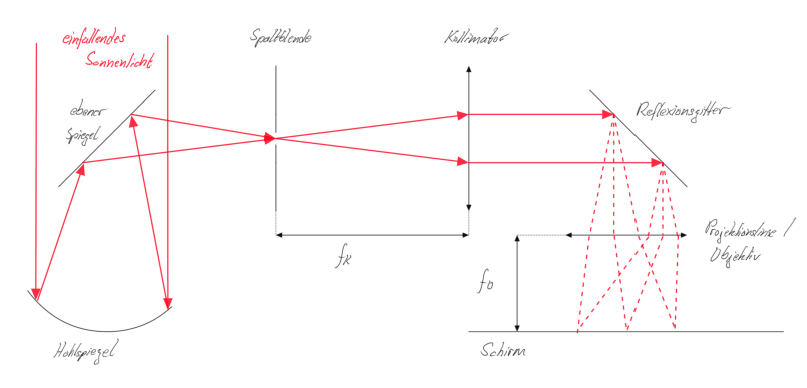
\includegraphics[scale=0.55]{skizzen/skizze-1.png}
			\caption{Skizze zum Aufbau des verwendeten Gitterspektrographen \\ $f_\mathrm{K}\ldots$Brennweite Kollimator \\ $f_\mathrm{O}\ldots$Brennweite Objektiv}
			\label{fig:skizze-spektrograph}
		\end{figure}

		Der grundsätzliche Aufbau des im Versuch verwendeten Gitterspektrographen ist in Abbildung \ref{fig:skizze-spektrograph} gezeigt.
		Hierbei wird das Sonnenlicht durch einen Hohlspiegel gebündelt und  durch eine Spaltblende zum Kollimator weitergeleitet.
		Durch den Spalt werden die Anteile des Lichts herausgefiltert, die nicht parallel zum Hohlspiegel eingefallen sind.
		Im Anschluss wird nun dieses divergierende Strahlenbündel mithilfe des Kollimators in ein rein paralleles Lichtbündel umgewandelt.
		Dieses trifft dann auf das Reflexionsgitter, welches wie ein typisches Gitter wirkt.
		Das Licht wird mit sich selbst interferieren, wodurch Beugungsmuster entstehen.
		Für große Entfernungen des Schirm interferieren näherungsweise parallele Strahlen miteinander.
		Die auftretenden Phänomene sind damit vergleichsweise leicht durch die Fraunhofer-Beugung berechenbar.
		Der Aufbau befindet sich jedoch in einem relativ kleinen geschlossenen System.
		Um die Bedingung, dass parallele Strahlen interferieren, dennoch nicht zu verletzen, werden durch eine Projektionslinse (auch Objektiv) parallel verlaufende Strahlen in einem Punkt auf dem Schirm fokussiert.
		Der Schirm zeigt also gerade die Spektrallinien des einfallendes Lichtes.

		Für den Abstand $x(n,\lambda)$ von der nullten Ordnung der Spektrallinie $n$.Ordnung mit Wellenlänge $\lambda$ ergibt sich dann näherungsweise
		\[ x(n,\lambda) = \frac{s}{g}n\lambda \]
		Dabei beschreibt $s$ den Abstand vom Gitter zum Schirm und $g$ die Gitterkonstante.
		Für das Auflösungsvermögen folgt dann
		\[ \frac{\lambda}{\Delta\lambda(n)} = \frac{x(n,\lambda)}{\Delta x(n,\lambda)} = nN \]
		wenn $N$ die Anzahl der beleuchteten Spalte am Reflexionsgitter beschreibt.

		Alle Berechnungen beruhen darauf, dass es sich um einen idealen Spektrographen handelt.
		Das heißt vor Allem, dass dabei die Spaltbreite der Spaltblende als gegen Null tendierend angenommen wird.
		Dies kann im Allgemeinen allerdings nicht realisiert werden, da sonst die Lichtintensität zu klein wäre.
		Aus diesem Grund wird das eigentliche Auflösungsvermögen stark durch die Spaltbreite bestimmt.
		Jede Spektrallinie ist dann eine Abbildung des Spalts.
	
	% subsection gitterspektrograph (end)

	\subsection{CCD-Detektor} % (fold)
	\label{sub:ccd_detektor}

		Um die Spektrallinien am Spektrograph messen zu können, wird der in Abbildung \ref{fig:skizze-spektrograph} beschriebene Schirm durch einen CCD-Detektor ersetzt.
		CCD-Detektoren bestehen aus einer Matrix lichtempfindlicher Fotodioden.
		Eine einfache Darstellung ist in Abbildung \ref{fig:schema-ccd} sichtbar.
		Einfallendes Licht überträgt durch den inneren photoelektrischen Effekt seine Energie auf die Elektronen der Halbleiter. 
		Dabei entstehen gleichzeitig negativ geladene freie Elektronen und positiv geladene \glqq Löcher\grqq, die sich aufgrund einer angelegten Spannung voneinander trennen. 
		Die Ladungen fließen jedoch nicht wie bei einer normalen Fotodiode sofort nach außen ab, sondern werden in der Speicherzelle selbst, in einem sogenannten Potentialtopf gesammelt, der wie ein Kondensator Ladungen speichert. 
		Die Ladungsmenge ist dabei proportional zur eingestrahlten Lichtmenge, wenn rechtzeitig ausgelesen wird, bevor die Leerlaufspannung der Fotodiode erreicht ist.
		Nach der Belichtung werden die Ladungen schrittweise verschoben, bis sie schließlich als Ladungspakete, eines nach dem anderen, den Ausleseverstärker erreichen. 
		Es wird eine von der Ladung und somit der Lichtmenge abhängige elektrische Spannung ausgegeben.
		Das Ausgangssignal des Sensors ist somit seriell.
		Durch Anwendung dieser Technik reicht es, bei der technischen Herstellung des CCD-Sensors einen Ausleseverstärker für die gesamte Matrix von Fotodioden zu verwenden.

		\begin{figure}
			\center
			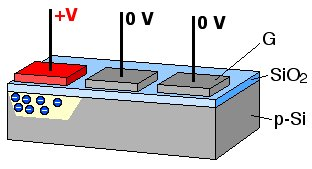
\includegraphics[scale=0.8]{referenzen/CCD_charge_transfer_animation.jpg}
			\caption{Schema eines CCD-Sensors (Quelle:\\ https://de.wikipedia.org/wiki/CCD-Sensor\#/media/File:CCD\_charge\_transfer\_animation.gif)}
			\label{fig:schema-ccd}
		\end{figure}

		Fotodioden eines CCD-Sensors können rechteckig, quadratisch oder polygonal sein, mit Kantenlängen von $1.4\unit{$\mu$m}$ bis über $20\unit{$\mu$m}$.
		Je größer die Fläche der Pixel, desto höher sind die Lichtempfindlichkeit und der Dynamikumfang, desto kleiner ist aber, bei gleicher Sensorgröße, die Bildauflösung.
		Bei Überbelichtung können Ladungen aus dem Potentialtopf einer Zelle in die Nachbarzellen übertreten.
		Die Messung von hohen Lichtintensitäten ist damit begrenzt.
		Abhilfe schaffte während des Versuches ein Papierfilter und die Einstellung einer kürzeren Belichtungszeit.

		Um nun mit dem CCD-Detektor auch Abstände oder Positionen messen zu können, muss ein bereits bekanntes Spektrum aufgenommen werden.
		So lassen sich dann mithilfe charakteristischer Spektrallinien die Skalierung $\alpha$ (Wellenlängenzunahme pro Pixel) und das Offset $\beta$ (Wellenlänge des linken äußersten Pixel) bestimmen.
		Näherungsweise können alle Funktionen als linear angesehen werden.
		Seien nun für zwei Wellenlängen $\lambda_1, \lambda_2$ mit $\lambda_1 < \lambda_2$ die Position bzw. die Pixel $p_1,p_2$ der Spektrallinien gegeben.
		Dann ergibt sich
		\begin{alignat*}{3}
			\alpha &= \frac{\lambda_2 - \lambda_1}{p_2 - p_1} \\
			\beta &= \lambda_1 - \alpha p_1
		\end{alignat*}
		Für die Wellenlänge eines beliebigen Pixels folgt dann, wenn alle Einstellungen am CCD-Detektor und am Spektrographen konstant bleiben
		\[ \lambda(p) = \alpha p + \beta \]
		Für gewisse Einstellungen und untersuchte Bereiche könnte diese Näherung verletzt werden.
		Um dies zu untersuchen, werden die gerade angegebenen Kalibrierungen nicht nur mit zwei Spektrallinien, sondern mit Mehreren an verschiedenen Stellen durchgeführt.

		Zur Auswertung der Intensitäten von Spektrallinien oder anderen Peaks ist es notwendig systematische und zufällige Fehler des CCD-Detektors zu kennen oder zu bestimmen.
		Hierfür spielen vor Allem die Kenngrößen Biaslevel, Rauschen und Dunkelstrom eine wichtige Rolle.
		
		Um ein Spannungssignal für verschiedene Pixel vom CCD-Sensor zu erhalten, werden, die Ladungen seriell ausgelesen, indem man die Ladungen von Diode zu Diode verschiebt.
		Bei dieser Verschiebung entsteht ein systematischer Fehler und eine statistische Abweichung (auch Rauschen) für jeden Pixel.
		Nach Beendigung des Auslesevorgangs wird zu jedem erhaltenen Wert ein sogenanntes Offset hinzuaddiert.
		Das Biaslevel eines Pixels ist dann gerade dieses Offset plus der systematische Fehler.

		Treffen keine Photonen auf den CCD-Sensor, so werden dennoch in jeder Fotodiode weitere Elektronen freigesetzt.
		Dieser Effekt entsteht durch die temperaturbedingte Bewegung der Elektronen, welche durch die geringe Bandlücke im Halbleiter ausreicht die Potentialbarriere zu überwinden.
		Die Anzahl der Elektronen pro Zeiteinheit, die so entstehen, wird Dunkelstrom genannt.
		Er ist jedoch unabhängig vom Photoneneinfall bzw. der Lichtintensität und somit ein Fehler in der Aufnahme.

	% subsection ccd_detektor (end)

	\subsection{Sonnenspektrum} % (fold)
	\label{sub:sonnenspektrum}

		Das elektromagnetische Spektrum der Sonne hat die größte Intensität im Bereich des sichtbaren Lichts. 
		Abhängig von der Wellenlänge wird die Sonnenstrahlung von der Atmosphäre mehr oder weniger stark absorbiert. 
		Die an der Erdoberfläche eintreffende Intensität hängt zudem stark vom Wetter und vom Sonnenstand ab.
		Beispiele des Sonnenspektrums zeigen die im Anhang \ref{sec:beispiele_des_sonnenspektrums} sichtbaren Abbildungen \ref{fig:sonnenspektrum-1} und \ref{fig:sonnenspektrum-2}.
		Das Spektrum ist von etwa $140 \unit{nm}$ bis etwa $10 \unit{cm}$ näherungsweise das eines Schwarzen Strahlers bei einer Temperatur von knapp $6000 \unit{K}$, der Temperatur der Photosphäre.
		Im Bereich von naher Infrarotstrahlung bis ins UV enthält das Spektrum eine Vielzahl von Absorptionslinien, die sogenannten Fraunhoferlinien. 
		Sie entstehen durch Strahlungsabsorption in der Chromosphäre der Sonne.
	
	% subsection sonnenspektrum (end)

% section grundlagen (end)
	\newpage
	\section{Versuchsaufbau und Durchführung} % (fold)
\label{sec:versuchsaufbau_und_durchf_hrung}

	\subsection{Aufbau des Michelson-Interferometers} % (fold)
	\label{sub:aufbau_des_michelson_interferometers}

	\begin{figure}[htb]
		\centering
		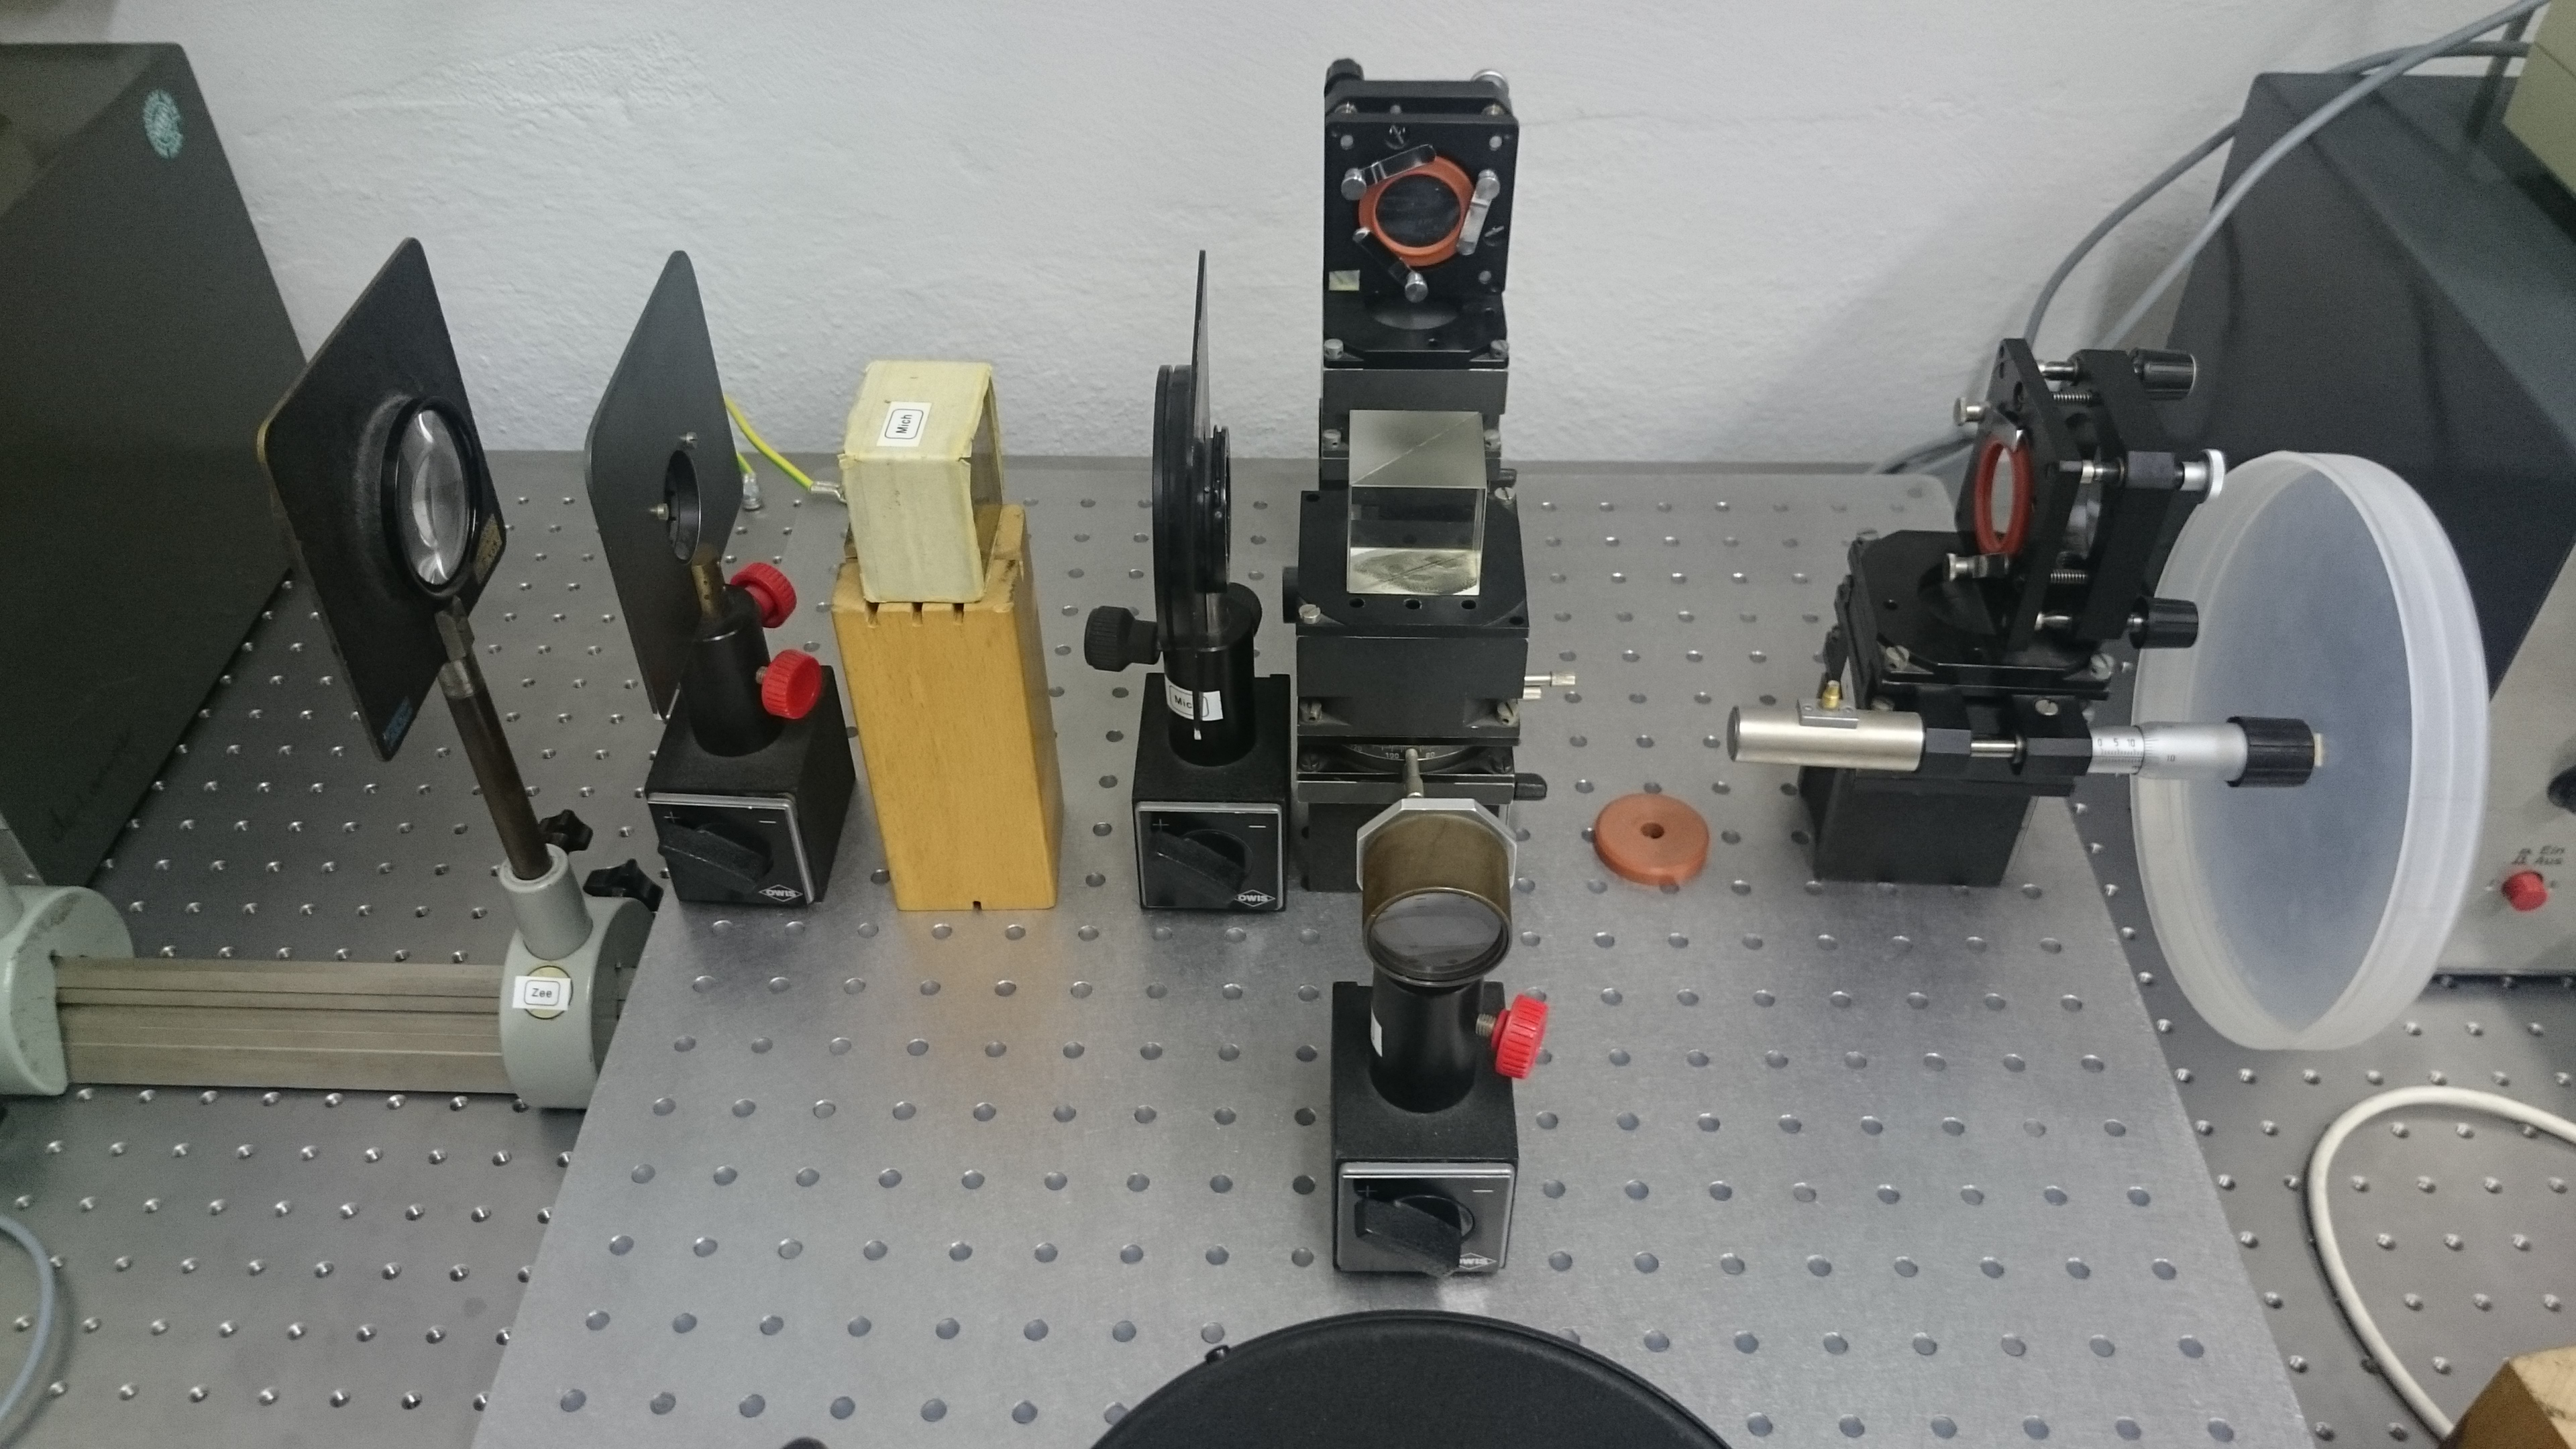
\includegraphics[scale = 0.08]{images/DSC_1011.JPG}
		\caption{Montagetisch mit Versuchsaufbau des MIF}
		\label{fig:aufbau-mif-1}
	\end{figure}

	In Abbildung \ref{fig:aufbau-mif-1} ist der Aufbau des MIF zu sehen, wie er unter Abschnitt \ref{sub:prinzip_des_michelson_interferometers} beschrieben wurde.
	Als Lichtquelle können eine Hg-Dampflampe mit verschiedenene Filtern sowie eine herkömmliche Glühlampe verwendet werden.
	Spiegel 2 ist über eine Mikrometerschraube in x-Richtung zu verstellen, drei weitere Feingewindeschrauben sind für die Winkeleinstellung vorgesehen.
	Durch Verwendung des Strahlteilerwürfels entfällt die sonst notwendige Kompensationsplatte.
	Neben der direkten Möglichkeit zur Beobachtung durch Blicken in den Strahlteiler, kann der Strahl auch noch mittels einer weiteren Linse und eines Ablenkspiegels auf Papier abgebildet und abfotografiert werden.
	
	% subsection aufbau_des_michelson_interferometers (end)


	\subsection{Aufbau des Fourier-Spektrometers} % (fold)
	\label{sub:aufabu_des_fourier_spektrometers}
	

	\begin{figure}[htb]
		\centering
		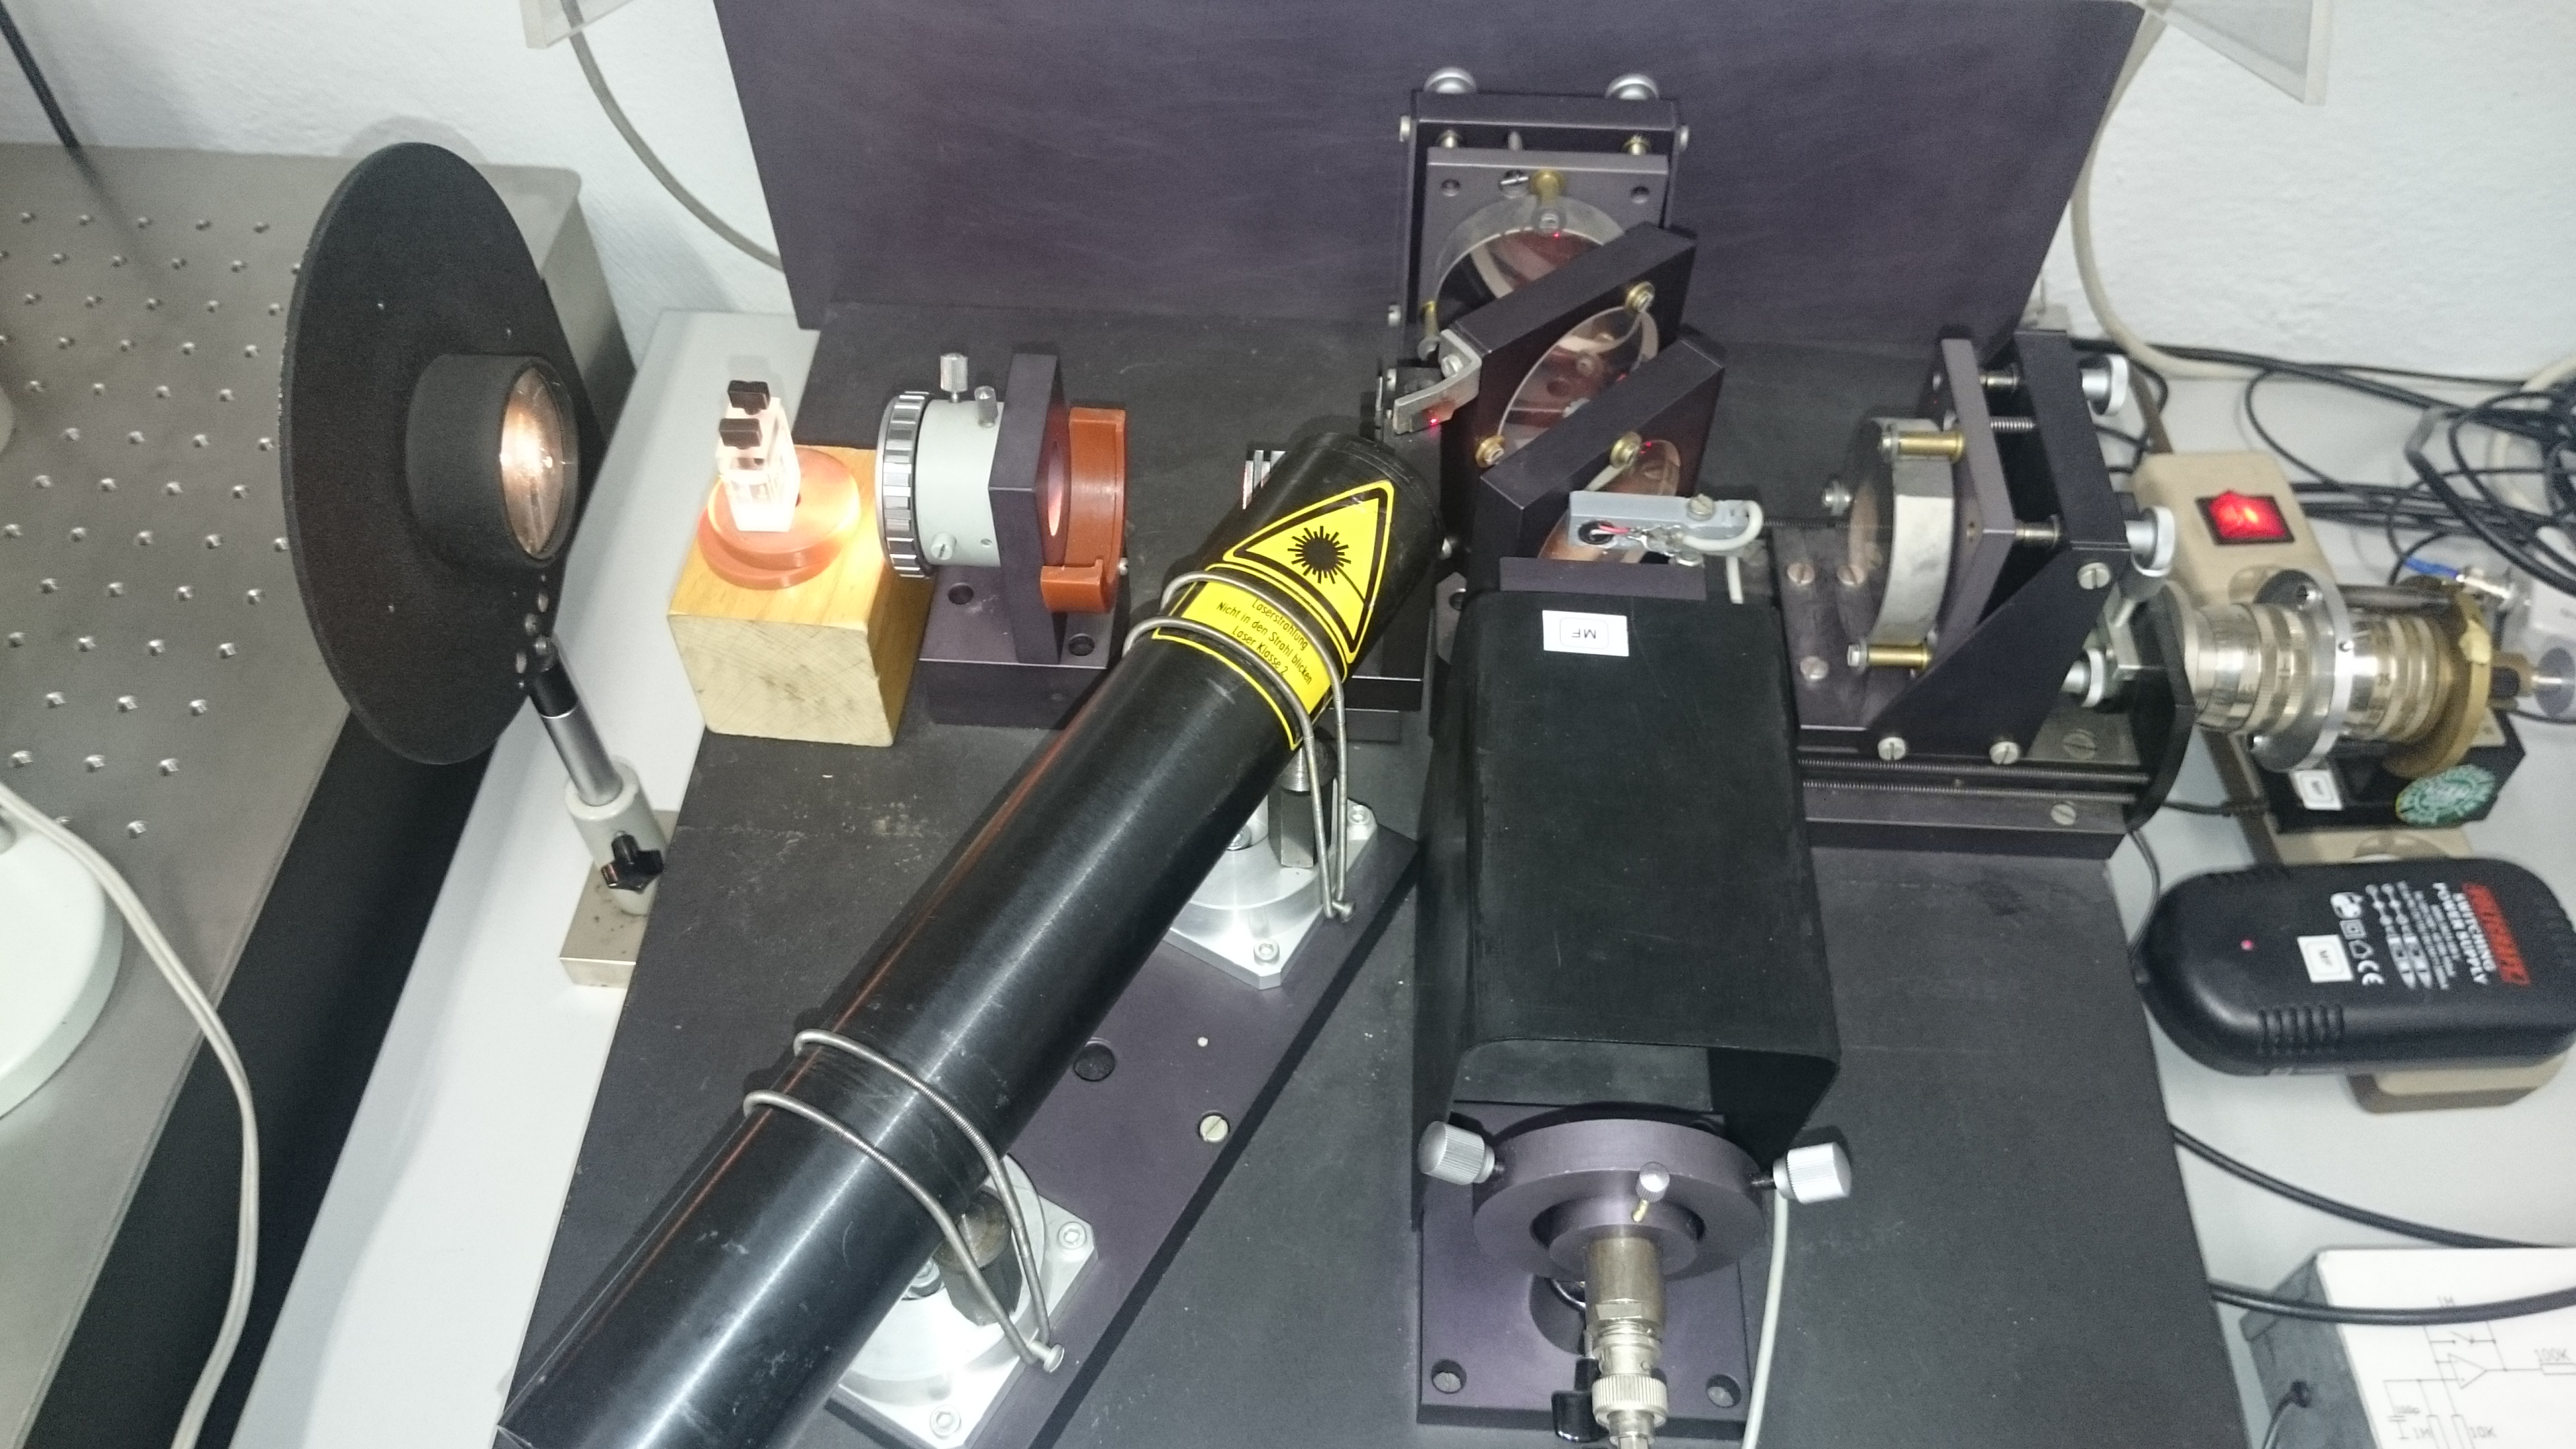
\includegraphics[scale = 0.08]{images/DSC_1010.JPG}
		\caption{Komponenten des Fourier-Spektrometers mit geöffneter Abdeckklappe}
		\label{fig:aufbau-mif-2}
	\end{figure}

	Abbildung \ref{fig:aufbau-mif-2} zeigt alle Komponeneten des Fourierspektrometers wie es im Versuch verwendet wurde.
	Links befindet sich die Lichtquelle.
	Als solche werden im Versuch Hg-Lampe, Na-Lampe, grüne LED, rote Laser-LED, Gas-Laser und Glühlampe verwendet.
	Zwischen Lampe und Kollimator können Filter oder Proben zur Absorbtion platziert werden.
	In der Mitte teilt ein halbdurchlässiger Spiegel den Strahl, kurz darüber ist die Kompensationsplatte zu finden.
	Spiegel 2 kann mittels einer Mikrometerschraube und den dahinter befindlichen Motor über den Computer gesteuert werden.
	Unter dem Strahlteiler befindet sich eine Linse, die den Strahl auf den Detektor bündelt.
	Auf der Linse befindet sich der Detektor für das Laser-Referenzsignal.
	An diesem wird die Messung anschließend angepasst und kalibriert.
	Akkumulierung der Datenpunkte, Aufzeichnen des Interferogramms und Erstellen der zugehörigen FFT (Fast Fourier Transformation) werden von einem LabView-Programm erledigt.
	Es dient ebenfalls zum Ansteuern des Motors von Spiegel 2.

	% subsection aufabu_des_fourier_spektrometers (end)


% section versuchsaufbau_und_durchf_hrung (end)
	\newpage
	\subsection{Probenstrombilder} % (fold)
\label{sub:probenstrombilder}
	
	Folgende Abbildung verdeutlicht, welche Proben an welchen Stellen analysiert wurden.

	\begin{figure}[H]
		\center
		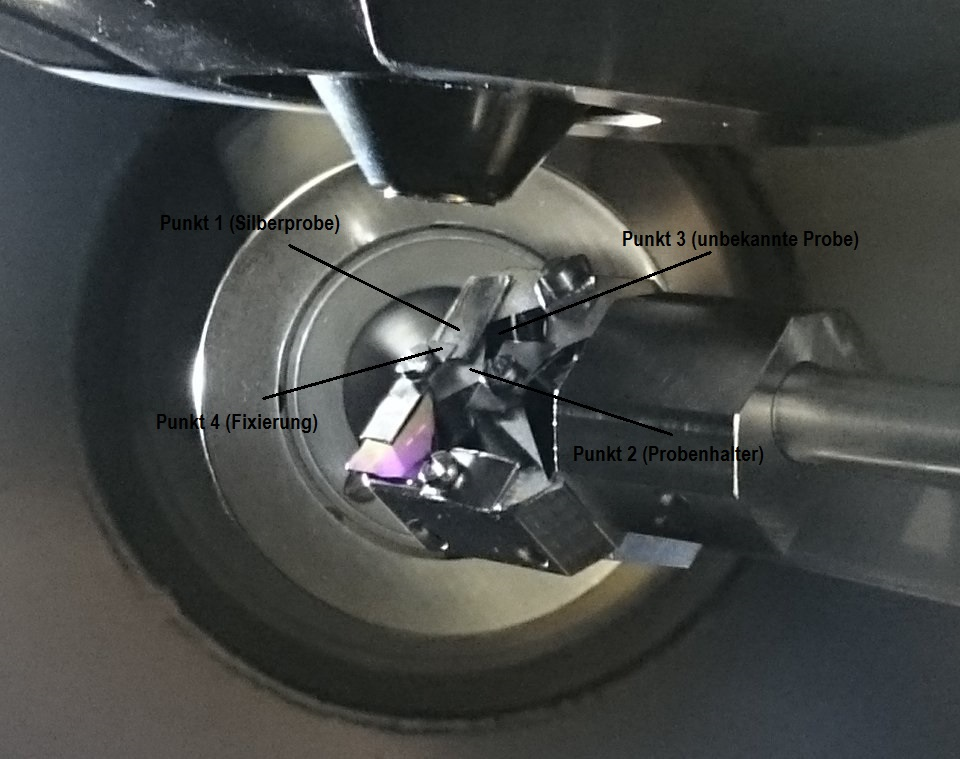
\includegraphics[scale=0.4]{probe_photo_Bear.jpg}
		\caption{\centering Bild des Probenhalters mit den untersuchten Proben \\ (Aufnahme durch eine Digitalkamera)}
	\end{figure}

	Dabei entstanden folgende Probenstrombilder:

	\begin{figure}[H]
		\center
		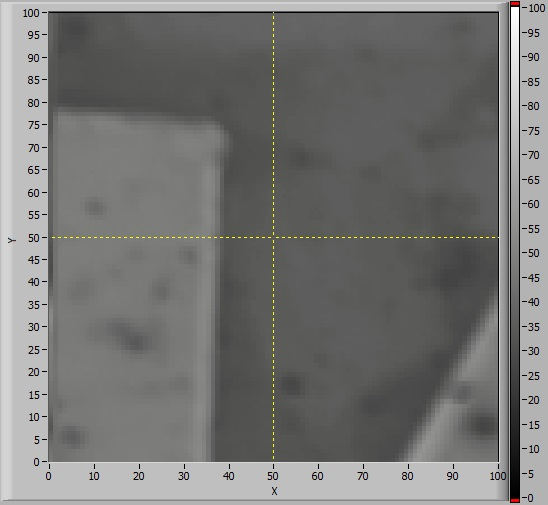
\includegraphics[scale=0.5]{epic01.jpg}
		\caption{\centering Probenstrombild von Silber (links) Probenhalter (Mitte) und Probe 3 (rechts) \\ Aufnahme mit 4keV und Probenstrom von ca. 43 nA}
	\end{figure}

	\begin{figure}[H]	
		\center
		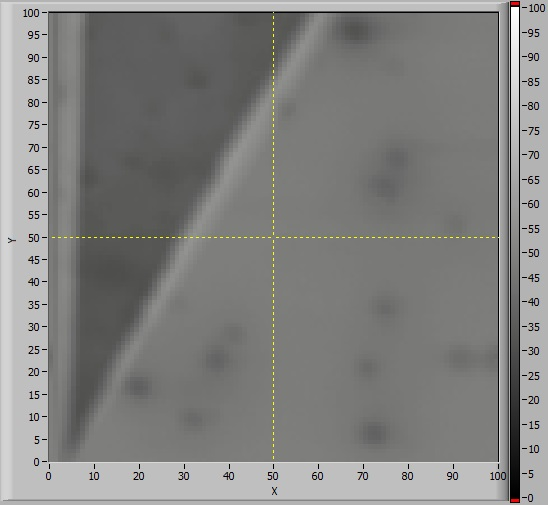
\includegraphics[scale=0.6]{epic02.jpg}
		\caption{\centering Probenstrombild von Probe 3 \\ Aufnahme mit 4keV und Probenstrom von ca. 130 nA}
	\end{figure}

	\begin{figure}[H]	
		\center
		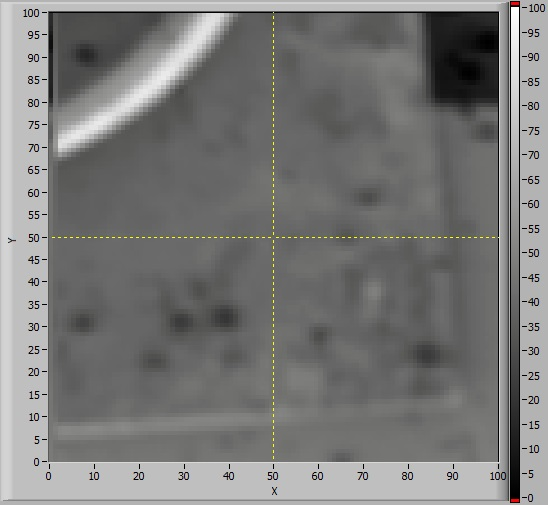
\includegraphics[scale=0.6]{epicSchraube.jpg}
		\caption{\centering Probenstrombild von Fixierung \\ Aufnahme mit 4keV und Probenstrom von ca. 110 nA}
	\end{figure}

	Die Aufnahmen stellen die jeweiligen Objekte immer horizontal gespiegelt dar. Der unterschiedliche Probenstrom deutet darauf hin, 
	dass je nach Untergrund die Elektronen mehr oder weniger stark gestreut wurden und nicht über Probe und Zählwerk zurück geleitet.

% subsection probenstrombilder (end)

\subsection{Silber-Spektrum, Messparameter und Geometriefaktor} % (fold)
\label{sub:silber_spektrum}

	\begin{figure}[H]
		\center
		% GNUPLOT: LaTeX picture with Postscript
\begingroup
  \makeatletter
  \providecommand\color[2][]{%
    \GenericError{(gnuplot) \space\space\space\@spaces}{%
      Package color not loaded in conjunction with
      terminal option `colourtext'%
    }{See the gnuplot documentation for explanation.%
    }{Either use 'blacktext' in gnuplot or load the package
      color.sty in LaTeX.}%
    \renewcommand\color[2][]{}%
  }%
  \providecommand\includegraphics[2][]{%
    \GenericError{(gnuplot) \space\space\space\@spaces}{%
      Package graphicx or graphics not loaded%
    }{See the gnuplot documentation for explanation.%
    }{The gnuplot epslatex terminal needs graphicx.sty or graphics.sty.}%
    \renewcommand\includegraphics[2][]{}%
  }%
  \providecommand\rotatebox[2]{#2}%
  \@ifundefined{ifGPcolor}{%
    \newif\ifGPcolor
    \GPcolorfalse
  }{}%
  \@ifundefined{ifGPblacktext}{%
    \newif\ifGPblacktext
    \GPblacktexttrue
  }{}%
  % define a \g@addto@macro without @ in the name:
  \let\gplgaddtomacro\g@addto@macro
  % define empty templates for all commands taking text:
  \gdef\gplbacktext{}%
  \gdef\gplfronttext{}%
  \makeatother
  \ifGPblacktext
    % no textcolor at all
    \def\colorrgb#1{}%
    \def\colorgray#1{}%
  \else
    % gray or color?
    \ifGPcolor
      \def\colorrgb#1{\color[rgb]{#1}}%
      \def\colorgray#1{\color[gray]{#1}}%
      \expandafter\def\csname LTw\endcsname{\color{white}}%
      \expandafter\def\csname LTb\endcsname{\color{black}}%
      \expandafter\def\csname LTa\endcsname{\color{black}}%
      \expandafter\def\csname LT0\endcsname{\color[rgb]{1,0,0}}%
      \expandafter\def\csname LT1\endcsname{\color[rgb]{0,1,0}}%
      \expandafter\def\csname LT2\endcsname{\color[rgb]{0,0,1}}%
      \expandafter\def\csname LT3\endcsname{\color[rgb]{1,0,1}}%
      \expandafter\def\csname LT4\endcsname{\color[rgb]{0,1,1}}%
      \expandafter\def\csname LT5\endcsname{\color[rgb]{1,1,0}}%
      \expandafter\def\csname LT6\endcsname{\color[rgb]{0,0,0}}%
      \expandafter\def\csname LT7\endcsname{\color[rgb]{1,0.3,0}}%
      \expandafter\def\csname LT8\endcsname{\color[rgb]{0.5,0.5,0.5}}%
    \else
      % gray
      \def\colorrgb#1{\color{black}}%
      \def\colorgray#1{\color[gray]{#1}}%
      \expandafter\def\csname LTw\endcsname{\color{white}}%
      \expandafter\def\csname LTb\endcsname{\color{black}}%
      \expandafter\def\csname LTa\endcsname{\color{black}}%
      \expandafter\def\csname LT0\endcsname{\color{black}}%
      \expandafter\def\csname LT1\endcsname{\color{black}}%
      \expandafter\def\csname LT2\endcsname{\color{black}}%
      \expandafter\def\csname LT3\endcsname{\color{black}}%
      \expandafter\def\csname LT4\endcsname{\color{black}}%
      \expandafter\def\csname LT5\endcsname{\color{black}}%
      \expandafter\def\csname LT6\endcsname{\color{black}}%
      \expandafter\def\csname LT7\endcsname{\color{black}}%
      \expandafter\def\csname LT8\endcsname{\color{black}}%
    \fi
  \fi
  \setlength{\unitlength}{0.0500bp}%
  \begin{picture}(9354.00,5102.00)%
    \gplgaddtomacro\gplbacktext{%
      \csname LTb\endcsname%
      \put(946,704){\makebox(0,0)[r]{\strut{}-2}}%
      \put(946,1171){\makebox(0,0)[r]{\strut{}-1.5}}%
      \put(946,1638){\makebox(0,0)[r]{\strut{}-1}}%
      \put(946,2105){\makebox(0,0)[r]{\strut{}-0.5}}%
      \put(946,2573){\makebox(0,0)[r]{\strut{} 0}}%
      \put(946,3040){\makebox(0,0)[r]{\strut{} 0.5}}%
      \put(946,3507){\makebox(0,0)[r]{\strut{} 1}}%
      \put(946,3974){\makebox(0,0)[r]{\strut{} 1.5}}%
      \put(946,4441){\makebox(0,0)[r]{\strut{} 2}}%
      \put(1078,484){\makebox(0,0){\strut{} 0}}%
      \put(2391,484){\makebox(0,0){\strut{} 100}}%
      \put(3704,484){\makebox(0,0){\strut{} 200}}%
      \put(5018,484){\makebox(0,0){\strut{} 300}}%
      \put(6331,484){\makebox(0,0){\strut{} 400}}%
      \put(7644,484){\makebox(0,0){\strut{} 500}}%
      \put(8957,484){\makebox(0,0){\strut{} 600}}%
      \put(176,2572){\rotatebox{-270}{\makebox(0,0){\strut{}$dN/dE \ [1]$}}}%
      \put(5017,154){\makebox(0,0){\strut{}$E \ [eV]$}}%
      \put(5017,4771){\makebox(0,0){\strut{}Ag-Spektrum}}%
    }%
    \gplgaddtomacro\gplfronttext{%
      \csname LTb\endcsname%
      \put(7970,4268){\makebox(0,0)[r]{\strut{}Messwerte}}%
    }%
    \gplbacktext
    \put(0,0){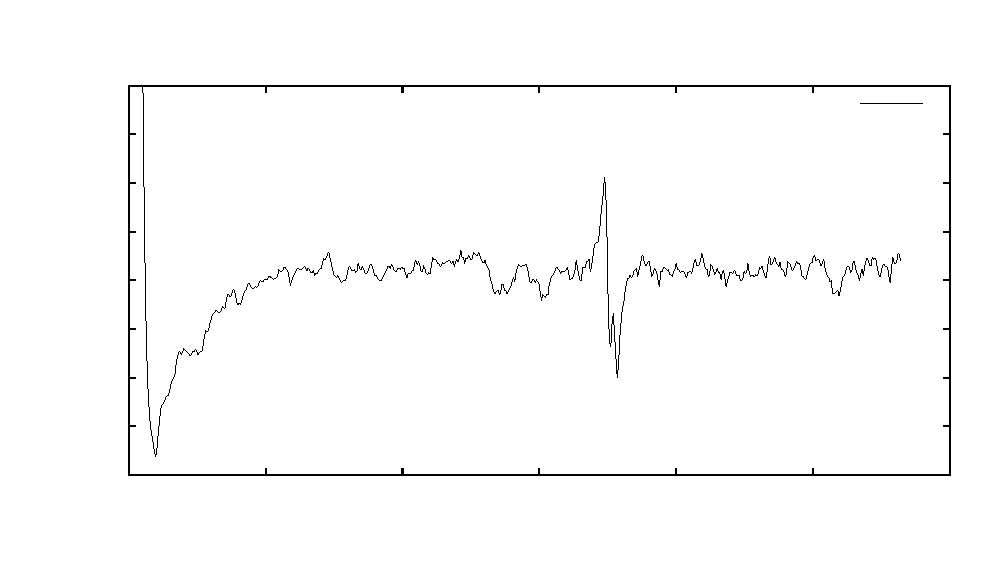
\includegraphics{ma03-16}}%
    \gplfronttext
  \end{picture}%
\endgroup

		\caption{\centering Parameter: Modulationsspannung 2V, AQ 120s, Empfindlichkeit 1mV, Zeitkonstante 300ms, Phase 12^\circ}
	\end{figure}

	\begin{figure}[H]
		\center
		% GNUPLOT: LaTeX picture with Postscript
\begingroup
  \makeatletter
  \providecommand\color[2][]{%
    \GenericError{(gnuplot) \space\space\space\@spaces}{%
      Package color not loaded in conjunction with
      terminal option `colourtext'%
    }{See the gnuplot documentation for explanation.%
    }{Either use 'blacktext' in gnuplot or load the package
      color.sty in LaTeX.}%
    \renewcommand\color[2][]{}%
  }%
  \providecommand\includegraphics[2][]{%
    \GenericError{(gnuplot) \space\space\space\@spaces}{%
      Package graphicx or graphics not loaded%
    }{See the gnuplot documentation for explanation.%
    }{The gnuplot epslatex terminal needs graphicx.sty or graphics.sty.}%
    \renewcommand\includegraphics[2][]{}%
  }%
  \providecommand\rotatebox[2]{#2}%
  \@ifundefined{ifGPcolor}{%
    \newif\ifGPcolor
    \GPcolorfalse
  }{}%
  \@ifundefined{ifGPblacktext}{%
    \newif\ifGPblacktext
    \GPblacktexttrue
  }{}%
  % define a \g@addto@macro without @ in the name:
  \let\gplgaddtomacro\g@addto@macro
  % define empty templates for all commands taking text:
  \gdef\gplbacktext{}%
  \gdef\gplfronttext{}%
  \makeatother
  \ifGPblacktext
    % no textcolor at all
    \def\colorrgb#1{}%
    \def\colorgray#1{}%
  \else
    % gray or color?
    \ifGPcolor
      \def\colorrgb#1{\color[rgb]{#1}}%
      \def\colorgray#1{\color[gray]{#1}}%
      \expandafter\def\csname LTw\endcsname{\color{white}}%
      \expandafter\def\csname LTb\endcsname{\color{black}}%
      \expandafter\def\csname LTa\endcsname{\color{black}}%
      \expandafter\def\csname LT0\endcsname{\color[rgb]{1,0,0}}%
      \expandafter\def\csname LT1\endcsname{\color[rgb]{0,1,0}}%
      \expandafter\def\csname LT2\endcsname{\color[rgb]{0,0,1}}%
      \expandafter\def\csname LT3\endcsname{\color[rgb]{1,0,1}}%
      \expandafter\def\csname LT4\endcsname{\color[rgb]{0,1,1}}%
      \expandafter\def\csname LT5\endcsname{\color[rgb]{1,1,0}}%
      \expandafter\def\csname LT6\endcsname{\color[rgb]{0,0,0}}%
      \expandafter\def\csname LT7\endcsname{\color[rgb]{1,0.3,0}}%
      \expandafter\def\csname LT8\endcsname{\color[rgb]{0.5,0.5,0.5}}%
    \else
      % gray
      \def\colorrgb#1{\color{black}}%
      \def\colorgray#1{\color[gray]{#1}}%
      \expandafter\def\csname LTw\endcsname{\color{white}}%
      \expandafter\def\csname LTb\endcsname{\color{black}}%
      \expandafter\def\csname LTa\endcsname{\color{black}}%
      \expandafter\def\csname LT0\endcsname{\color{black}}%
      \expandafter\def\csname LT1\endcsname{\color{black}}%
      \expandafter\def\csname LT2\endcsname{\color{black}}%
      \expandafter\def\csname LT3\endcsname{\color{black}}%
      \expandafter\def\csname LT4\endcsname{\color{black}}%
      \expandafter\def\csname LT5\endcsname{\color{black}}%
      \expandafter\def\csname LT6\endcsname{\color{black}}%
      \expandafter\def\csname LT7\endcsname{\color{black}}%
      \expandafter\def\csname LT8\endcsname{\color{black}}%
    \fi
  \fi
  \setlength{\unitlength}{0.0500bp}%
  \begin{picture}(9354.00,5102.00)%
    \gplgaddtomacro\gplbacktext{%
      \csname LTb\endcsname%
      \put(946,704){\makebox(0,0)[r]{\strut{}-2}}%
      \put(946,1238){\makebox(0,0)[r]{\strut{}-1.5}}%
      \put(946,1772){\makebox(0,0)[r]{\strut{}-1}}%
      \put(946,2306){\makebox(0,0)[r]{\strut{}-0.5}}%
      \put(946,2839){\makebox(0,0)[r]{\strut{} 0}}%
      \put(946,3373){\makebox(0,0)[r]{\strut{} 0.5}}%
      \put(946,3907){\makebox(0,0)[r]{\strut{} 1}}%
      \put(946,4441){\makebox(0,0)[r]{\strut{} 1.5}}%
      \put(1078,484){\makebox(0,0){\strut{} 310}}%
      \put(1953,484){\makebox(0,0){\strut{} 320}}%
      \put(2829,484){\makebox(0,0){\strut{} 330}}%
      \put(3704,484){\makebox(0,0){\strut{} 340}}%
      \put(4580,484){\makebox(0,0){\strut{} 350}}%
      \put(5455,484){\makebox(0,0){\strut{} 360}}%
      \put(6331,484){\makebox(0,0){\strut{} 370}}%
      \put(7206,484){\makebox(0,0){\strut{} 380}}%
      \put(8082,484){\makebox(0,0){\strut{} 390}}%
      \put(8957,484){\makebox(0,0){\strut{} 400}}%
      \put(176,2572){\rotatebox{-270}{\makebox(0,0){\strut{}$dN/dE \ [1]$}}}%
      \put(5017,154){\makebox(0,0){\strut{}$E \ [eV]$}}%
      \put(5017,4771){\makebox(0,0){\strut{}Ag-Spektrum}}%
    }%
    \gplgaddtomacro\gplfronttext{%
      \csname LTb\endcsname%
      \put(7970,4268){\makebox(0,0)[r]{\strut{}Messwerte}}%
    }%
    \gplbacktext
    \put(0,0){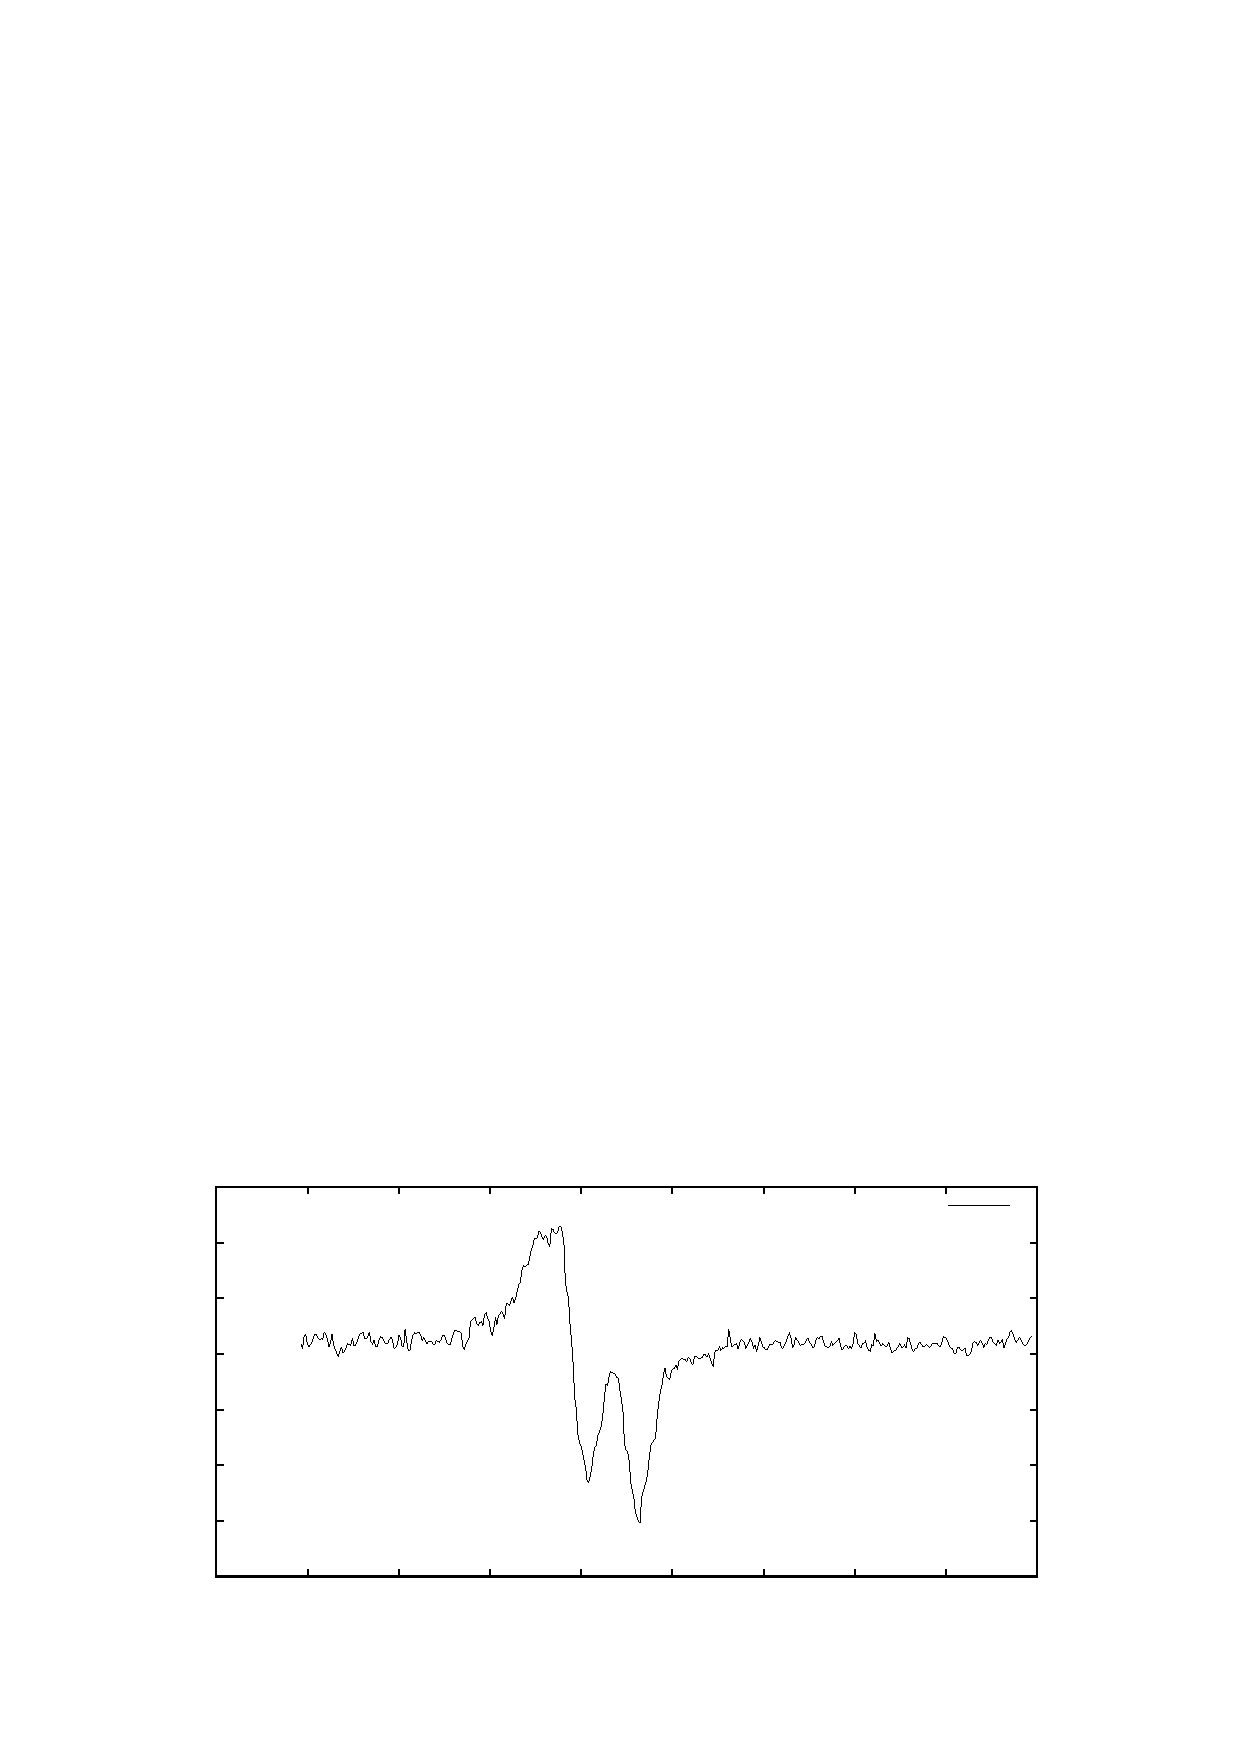
\includegraphics{ma03-15}}%
    \gplfronttext
  \end{picture}%
\endgroup

		\caption{\centering Parameter: Modulationsspannung 2V, AQ 120s, Empfindlichkeit 1mV, Zeitkonstante 300ms, Phase 12^\circ}
	\end{figure}

	Zu sehen ist das Auger-Elektronen-Spektrum von Silber (Ag) in differentieller Form in einem CMA-Spannungsbereich von 0 bis 350 V.
	Und damit in einem Energiebereich von 0 bis 570 eV (Geometriefaktor K = 1,624 siehe unten).
	Gut zu erkennen ist der charakteristische Doppelpeak. 
	Die beiden Minima sind im vergrößertem Ausschnitt abzulesen:

	Dabei konnten im verwendeten Messprogramm folgende Werte abgelesen werden:
	\begin{itemize}
		\item
			$U_{min}^{(1)} = 216.0V$ 
		\item
			$U_{min}^{(2)} = 219.4V$
	\end{itemize}

	Der Geometriefaktor K wurde anhand dieser beiden Peaks und den zugehörigen Tabellenwerten 351eV bzw. 356eV bestimmt (dem Katalog am Versuchsplatz entnommen):
	\begin{itemize}
		\item
			$K_1 = \dfrac{351}{216.0} = 1.625$
		\item
			$K_2 = \dfrac{356}{219.4} = 1.623$
	\end{itemize}
	\[
		\Rightarrow \={K} = 1.624
	\]
	Alle weiteren Auger-Spektren wurden mit diesem Geometriefaktor skaliert.
	Im Folgenden soll nun der Einfluss der verschiedenen Messparameter betrachtet werden.

	\subsubsection{Modulationsspannung} % (fold)
	\label{ssub:modulationsspannung}
	
		\begin{figure}[H]
			\center
			% GNUPLOT: LaTeX picture with Postscript
\begingroup
  \makeatletter
  \providecommand\color[2][]{%
    \GenericError{(gnuplot) \space\space\space\@spaces}{%
      Package color not loaded in conjunction with
      terminal option `colourtext'%
    }{See the gnuplot documentation for explanation.%
    }{Either use 'blacktext' in gnuplot or load the package
      color.sty in LaTeX.}%
    \renewcommand\color[2][]{}%
  }%
  \providecommand\includegraphics[2][]{%
    \GenericError{(gnuplot) \space\space\space\@spaces}{%
      Package graphicx or graphics not loaded%
    }{See the gnuplot documentation for explanation.%
    }{The gnuplot epslatex terminal needs graphicx.sty or graphics.sty.}%
    \renewcommand\includegraphics[2][]{}%
  }%
  \providecommand\rotatebox[2]{#2}%
  \@ifundefined{ifGPcolor}{%
    \newif\ifGPcolor
    \GPcolorfalse
  }{}%
  \@ifundefined{ifGPblacktext}{%
    \newif\ifGPblacktext
    \GPblacktexttrue
  }{}%
  % define a \g@addto@macro without @ in the name:
  \let\gplgaddtomacro\g@addto@macro
  % define empty templates for all commands taking text:
  \gdef\gplbacktext{}%
  \gdef\gplfronttext{}%
  \makeatother
  \ifGPblacktext
    % no textcolor at all
    \def\colorrgb#1{}%
    \def\colorgray#1{}%
  \else
    % gray or color?
    \ifGPcolor
      \def\colorrgb#1{\color[rgb]{#1}}%
      \def\colorgray#1{\color[gray]{#1}}%
      \expandafter\def\csname LTw\endcsname{\color{white}}%
      \expandafter\def\csname LTb\endcsname{\color{black}}%
      \expandafter\def\csname LTa\endcsname{\color{black}}%
      \expandafter\def\csname LT0\endcsname{\color[rgb]{1,0,0}}%
      \expandafter\def\csname LT1\endcsname{\color[rgb]{0,1,0}}%
      \expandafter\def\csname LT2\endcsname{\color[rgb]{0,0,1}}%
      \expandafter\def\csname LT3\endcsname{\color[rgb]{1,0,1}}%
      \expandafter\def\csname LT4\endcsname{\color[rgb]{0,1,1}}%
      \expandafter\def\csname LT5\endcsname{\color[rgb]{1,1,0}}%
      \expandafter\def\csname LT6\endcsname{\color[rgb]{0,0,0}}%
      \expandafter\def\csname LT7\endcsname{\color[rgb]{1,0.3,0}}%
      \expandafter\def\csname LT8\endcsname{\color[rgb]{0.5,0.5,0.5}}%
    \else
      % gray
      \def\colorrgb#1{\color{black}}%
      \def\colorgray#1{\color[gray]{#1}}%
      \expandafter\def\csname LTw\endcsname{\color{white}}%
      \expandafter\def\csname LTb\endcsname{\color{black}}%
      \expandafter\def\csname LTa\endcsname{\color{black}}%
      \expandafter\def\csname LT0\endcsname{\color{black}}%
      \expandafter\def\csname LT1\endcsname{\color{black}}%
      \expandafter\def\csname LT2\endcsname{\color{black}}%
      \expandafter\def\csname LT3\endcsname{\color{black}}%
      \expandafter\def\csname LT4\endcsname{\color{black}}%
      \expandafter\def\csname LT5\endcsname{\color{black}}%
      \expandafter\def\csname LT6\endcsname{\color{black}}%
      \expandafter\def\csname LT7\endcsname{\color{black}}%
      \expandafter\def\csname LT8\endcsname{\color{black}}%
    \fi
  \fi
  \setlength{\unitlength}{0.0500bp}%
  \begin{picture}(9354.00,5102.00)%
    \gplgaddtomacro\gplbacktext{%
      \csname LTb\endcsname%
      \put(682,704){\makebox(0,0)[r]{\strut{}-4}}%
      \put(682,1171){\makebox(0,0)[r]{\strut{}-3}}%
      \put(682,1638){\makebox(0,0)[r]{\strut{}-2}}%
      \put(682,2105){\makebox(0,0)[r]{\strut{}-1}}%
      \put(682,2573){\makebox(0,0)[r]{\strut{} 0}}%
      \put(682,3040){\makebox(0,0)[r]{\strut{} 1}}%
      \put(682,3507){\makebox(0,0)[r]{\strut{} 2}}%
      \put(682,3974){\makebox(0,0)[r]{\strut{} 3}}%
      \put(682,4441){\makebox(0,0)[r]{\strut{} 4}}%
      \put(814,484){\makebox(0,0){\strut{} 0}}%
      \put(2171,484){\makebox(0,0){\strut{} 100}}%
      \put(3528,484){\makebox(0,0){\strut{} 200}}%
      \put(4886,484){\makebox(0,0){\strut{} 300}}%
      \put(6243,484){\makebox(0,0){\strut{} 400}}%
      \put(7600,484){\makebox(0,0){\strut{} 500}}%
      \put(8957,484){\makebox(0,0){\strut{} 600}}%
      \put(176,2572){\rotatebox{-270}{\makebox(0,0){\strut{}$dN/dE \ [1]$}}}%
      \put(4885,154){\makebox(0,0){\strut{}$E \ [eV]$}}%
      \put(4885,4771){\makebox(0,0){\strut{}Ag-Spektrum mit Modulationsspannung $2V$}}%
    }%
    \gplgaddtomacro\gplfronttext{%
      \csname LTb\endcsname%
      \put(7970,4268){\makebox(0,0)[r]{\strut{}Messwerte}}%
    }%
    \gplbacktext
    \put(0,0){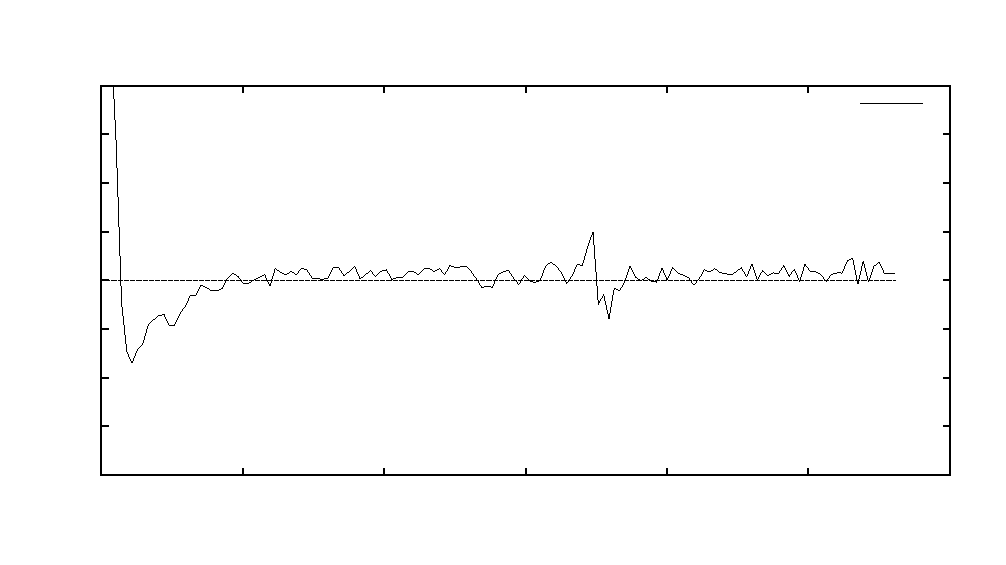
\includegraphics{ma03-01}}%
    \gplfronttext
  \end{picture}%
\endgroup

			\caption{\centering Parameter: AQ 30s, Empfindlichkeit 1mV, Zeitkonstante 100ms, Phase 0^\circ}
		\end{figure}

		\begin{figure}[H]
			\center
			% GNUPLOT: LaTeX picture with Postscript
\begingroup
  \makeatletter
  \providecommand\color[2][]{%
    \GenericError{(gnuplot) \space\space\space\@spaces}{%
      Package color not loaded in conjunction with
      terminal option `colourtext'%
    }{See the gnuplot documentation for explanation.%
    }{Either use 'blacktext' in gnuplot or load the package
      color.sty in LaTeX.}%
    \renewcommand\color[2][]{}%
  }%
  \providecommand\includegraphics[2][]{%
    \GenericError{(gnuplot) \space\space\space\@spaces}{%
      Package graphicx or graphics not loaded%
    }{See the gnuplot documentation for explanation.%
    }{The gnuplot epslatex terminal needs graphicx.sty or graphics.sty.}%
    \renewcommand\includegraphics[2][]{}%
  }%
  \providecommand\rotatebox[2]{#2}%
  \@ifundefined{ifGPcolor}{%
    \newif\ifGPcolor
    \GPcolorfalse
  }{}%
  \@ifundefined{ifGPblacktext}{%
    \newif\ifGPblacktext
    \GPblacktexttrue
  }{}%
  % define a \g@addto@macro without @ in the name:
  \let\gplgaddtomacro\g@addto@macro
  % define empty templates for all commands taking text:
  \gdef\gplbacktext{}%
  \gdef\gplfronttext{}%
  \makeatother
  \ifGPblacktext
    % no textcolor at all
    \def\colorrgb#1{}%
    \def\colorgray#1{}%
  \else
    % gray or color?
    \ifGPcolor
      \def\colorrgb#1{\color[rgb]{#1}}%
      \def\colorgray#1{\color[gray]{#1}}%
      \expandafter\def\csname LTw\endcsname{\color{white}}%
      \expandafter\def\csname LTb\endcsname{\color{black}}%
      \expandafter\def\csname LTa\endcsname{\color{black}}%
      \expandafter\def\csname LT0\endcsname{\color[rgb]{1,0,0}}%
      \expandafter\def\csname LT1\endcsname{\color[rgb]{0,1,0}}%
      \expandafter\def\csname LT2\endcsname{\color[rgb]{0,0,1}}%
      \expandafter\def\csname LT3\endcsname{\color[rgb]{1,0,1}}%
      \expandafter\def\csname LT4\endcsname{\color[rgb]{0,1,1}}%
      \expandafter\def\csname LT5\endcsname{\color[rgb]{1,1,0}}%
      \expandafter\def\csname LT6\endcsname{\color[rgb]{0,0,0}}%
      \expandafter\def\csname LT7\endcsname{\color[rgb]{1,0.3,0}}%
      \expandafter\def\csname LT8\endcsname{\color[rgb]{0.5,0.5,0.5}}%
    \else
      % gray
      \def\colorrgb#1{\color{black}}%
      \def\colorgray#1{\color[gray]{#1}}%
      \expandafter\def\csname LTw\endcsname{\color{white}}%
      \expandafter\def\csname LTb\endcsname{\color{black}}%
      \expandafter\def\csname LTa\endcsname{\color{black}}%
      \expandafter\def\csname LT0\endcsname{\color{black}}%
      \expandafter\def\csname LT1\endcsname{\color{black}}%
      \expandafter\def\csname LT2\endcsname{\color{black}}%
      \expandafter\def\csname LT3\endcsname{\color{black}}%
      \expandafter\def\csname LT4\endcsname{\color{black}}%
      \expandafter\def\csname LT5\endcsname{\color{black}}%
      \expandafter\def\csname LT6\endcsname{\color{black}}%
      \expandafter\def\csname LT7\endcsname{\color{black}}%
      \expandafter\def\csname LT8\endcsname{\color{black}}%
    \fi
  \fi
  \setlength{\unitlength}{0.0500bp}%
  \begin{picture}(9354.00,5102.00)%
    \gplgaddtomacro\gplbacktext{%
      \csname LTb\endcsname%
      \put(682,704){\makebox(0,0)[r]{\strut{}-4}}%
      \put(682,1171){\makebox(0,0)[r]{\strut{}-3}}%
      \put(682,1638){\makebox(0,0)[r]{\strut{}-2}}%
      \put(682,2105){\makebox(0,0)[r]{\strut{}-1}}%
      \put(682,2573){\makebox(0,0)[r]{\strut{} 0}}%
      \put(682,3040){\makebox(0,0)[r]{\strut{} 1}}%
      \put(682,3507){\makebox(0,0)[r]{\strut{} 2}}%
      \put(682,3974){\makebox(0,0)[r]{\strut{} 3}}%
      \put(682,4441){\makebox(0,0)[r]{\strut{} 4}}%
      \put(814,484){\makebox(0,0){\strut{} 0}}%
      \put(2171,484){\makebox(0,0){\strut{} 100}}%
      \put(3528,484){\makebox(0,0){\strut{} 200}}%
      \put(4886,484){\makebox(0,0){\strut{} 300}}%
      \put(6243,484){\makebox(0,0){\strut{} 400}}%
      \put(7600,484){\makebox(0,0){\strut{} 500}}%
      \put(8957,484){\makebox(0,0){\strut{} 600}}%
      \put(176,2572){\rotatebox{-270}{\makebox(0,0){\strut{}$dN/dE \ [1]$}}}%
      \put(4885,154){\makebox(0,0){\strut{}$E \ [eV]$}}%
      \put(4885,4771){\makebox(0,0){\strut{}Ag-Spektrum mit Modulationsspannung $5V$}}%
    }%
    \gplgaddtomacro\gplfronttext{%
      \csname LTb\endcsname%
      \put(7970,4268){\makebox(0,0)[r]{\strut{}Messwerte}}%
    }%
    \gplbacktext
    \put(0,0){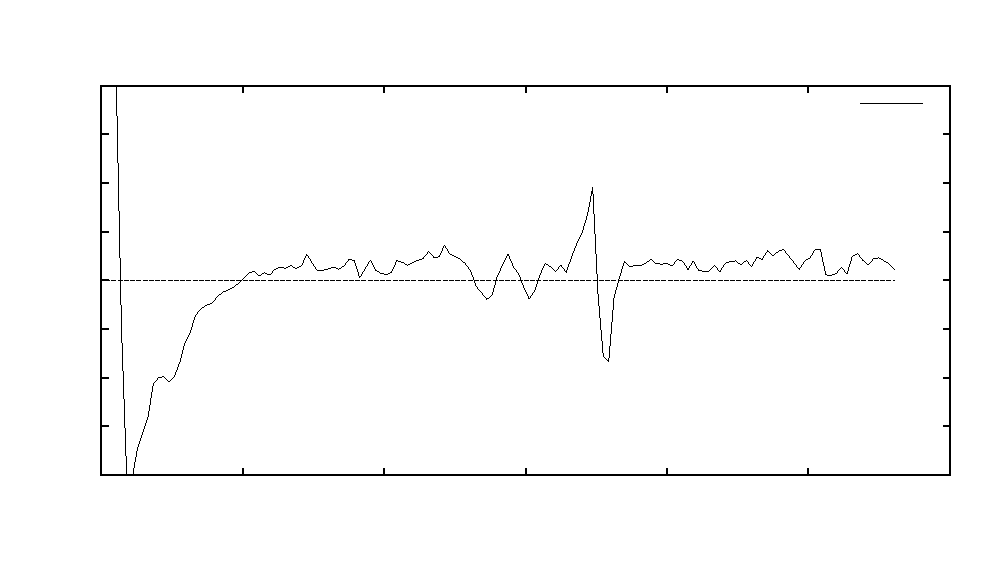
\includegraphics{ma03-02}}%
    \gplfronttext
  \end{picture}%
\endgroup

			\caption{\centering Parameter: AQ 30s, Empfindlichkeit 1mV, Zeitkonstante 100ms, Phase 0^\circ}	
		\end{figure}

		\begin{figure}[H]
			\center
			% GNUPLOT: LaTeX picture with Postscript
\begingroup
  \makeatletter
  \providecommand\color[2][]{%
    \GenericError{(gnuplot) \space\space\space\@spaces}{%
      Package color not loaded in conjunction with
      terminal option `colourtext'%
    }{See the gnuplot documentation for explanation.%
    }{Either use 'blacktext' in gnuplot or load the package
      color.sty in LaTeX.}%
    \renewcommand\color[2][]{}%
  }%
  \providecommand\includegraphics[2][]{%
    \GenericError{(gnuplot) \space\space\space\@spaces}{%
      Package graphicx or graphics not loaded%
    }{See the gnuplot documentation for explanation.%
    }{The gnuplot epslatex terminal needs graphicx.sty or graphics.sty.}%
    \renewcommand\includegraphics[2][]{}%
  }%
  \providecommand\rotatebox[2]{#2}%
  \@ifundefined{ifGPcolor}{%
    \newif\ifGPcolor
    \GPcolorfalse
  }{}%
  \@ifundefined{ifGPblacktext}{%
    \newif\ifGPblacktext
    \GPblacktexttrue
  }{}%
  % define a \g@addto@macro without @ in the name:
  \let\gplgaddtomacro\g@addto@macro
  % define empty templates for all commands taking text:
  \gdef\gplbacktext{}%
  \gdef\gplfronttext{}%
  \makeatother
  \ifGPblacktext
    % no textcolor at all
    \def\colorrgb#1{}%
    \def\colorgray#1{}%
  \else
    % gray or color?
    \ifGPcolor
      \def\colorrgb#1{\color[rgb]{#1}}%
      \def\colorgray#1{\color[gray]{#1}}%
      \expandafter\def\csname LTw\endcsname{\color{white}}%
      \expandafter\def\csname LTb\endcsname{\color{black}}%
      \expandafter\def\csname LTa\endcsname{\color{black}}%
      \expandafter\def\csname LT0\endcsname{\color[rgb]{1,0,0}}%
      \expandafter\def\csname LT1\endcsname{\color[rgb]{0,1,0}}%
      \expandafter\def\csname LT2\endcsname{\color[rgb]{0,0,1}}%
      \expandafter\def\csname LT3\endcsname{\color[rgb]{1,0,1}}%
      \expandafter\def\csname LT4\endcsname{\color[rgb]{0,1,1}}%
      \expandafter\def\csname LT5\endcsname{\color[rgb]{1,1,0}}%
      \expandafter\def\csname LT6\endcsname{\color[rgb]{0,0,0}}%
      \expandafter\def\csname LT7\endcsname{\color[rgb]{1,0.3,0}}%
      \expandafter\def\csname LT8\endcsname{\color[rgb]{0.5,0.5,0.5}}%
    \else
      % gray
      \def\colorrgb#1{\color{black}}%
      \def\colorgray#1{\color[gray]{#1}}%
      \expandafter\def\csname LTw\endcsname{\color{white}}%
      \expandafter\def\csname LTb\endcsname{\color{black}}%
      \expandafter\def\csname LTa\endcsname{\color{black}}%
      \expandafter\def\csname LT0\endcsname{\color{black}}%
      \expandafter\def\csname LT1\endcsname{\color{black}}%
      \expandafter\def\csname LT2\endcsname{\color{black}}%
      \expandafter\def\csname LT3\endcsname{\color{black}}%
      \expandafter\def\csname LT4\endcsname{\color{black}}%
      \expandafter\def\csname LT5\endcsname{\color{black}}%
      \expandafter\def\csname LT6\endcsname{\color{black}}%
      \expandafter\def\csname LT7\endcsname{\color{black}}%
      \expandafter\def\csname LT8\endcsname{\color{black}}%
    \fi
  \fi
  \setlength{\unitlength}{0.0500bp}%
  \begin{picture}(9354.00,5102.00)%
    \gplgaddtomacro\gplbacktext{%
      \csname LTb\endcsname%
      \put(682,704){\makebox(0,0)[r]{\strut{}-4}}%
      \put(682,1171){\makebox(0,0)[r]{\strut{}-3}}%
      \put(682,1638){\makebox(0,0)[r]{\strut{}-2}}%
      \put(682,2105){\makebox(0,0)[r]{\strut{}-1}}%
      \put(682,2573){\makebox(0,0)[r]{\strut{} 0}}%
      \put(682,3040){\makebox(0,0)[r]{\strut{} 1}}%
      \put(682,3507){\makebox(0,0)[r]{\strut{} 2}}%
      \put(682,3974){\makebox(0,0)[r]{\strut{} 3}}%
      \put(682,4441){\makebox(0,0)[r]{\strut{} 4}}%
      \put(814,484){\makebox(0,0){\strut{} 0}}%
      \put(2171,484){\makebox(0,0){\strut{} 100}}%
      \put(3528,484){\makebox(0,0){\strut{} 200}}%
      \put(4886,484){\makebox(0,0){\strut{} 300}}%
      \put(6243,484){\makebox(0,0){\strut{} 400}}%
      \put(7600,484){\makebox(0,0){\strut{} 500}}%
      \put(8957,484){\makebox(0,0){\strut{} 600}}%
      \put(176,2572){\rotatebox{-270}{\makebox(0,0){\strut{}$dN/dE \ [1]$}}}%
      \put(4885,154){\makebox(0,0){\strut{}$E \ [eV]$}}%
      \put(4885,4771){\makebox(0,0){\strut{}Ag-Spektrummit Modulationsspannung 10V}}%
    }%
    \gplgaddtomacro\gplfronttext{%
      \csname LTb\endcsname%
      \put(7970,4268){\makebox(0,0)[r]{\strut{}Messwerte}}%
    }%
    \gplbacktext
    \put(0,0){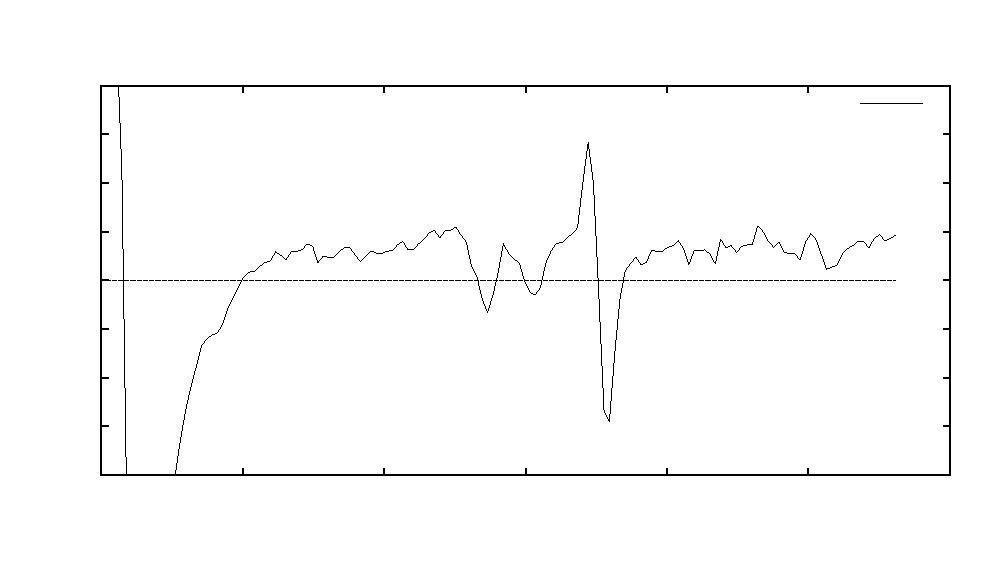
\includegraphics{ma03-03}}%
    \gplfronttext
  \end{picture}%
\endgroup

			\caption{\centering Parameter: AQ 30s, Empfindlichkeit 1mV, Zeitkonstante 100ms, Phase 0^\circ}
		\end{figure}
	
		Betrachtet man Peak-Höhe und Rauschen so fällt auf, dass die Silberpeaks bei 5V doppelt so hoch sind (bei gleicher Empfindlichkeit, Skalierung etc.), wie bei 2V.
		Dagegen hat das Rauschen nur minimal bis nicht zugenommen hat. 
		Allerdings zeigt sich auf vielen Bildern mit 10V Modulation, dass das Rauschen zwar nicht unbedingt an Intensität zunimmt, aber die Kurven im Allgemeinen nach oben verschoben ist. 
		Auf jeden Fall lässt sich durch höhere Modulationsspannung ein besseres Signal/Rausch-Verhältnis erhalten.
		Damit verstärken sich die Extrema, wobei jedoch zu beachten ist, dass keine Peak Abstände unterhalb der Modulationsspannung mehr aufgelöst werden können, da über diese hinweg gemittelt wird. 
		Die Kurve wird also glatter.

	% subsubsection modulationsspannung (end)

	\subsubsection{Zeitkonstante} % (fold)
	\label{ssub:zeitkonstante}
	
		Die Zeitkonstante stellt ein Maß dafür da, über wie viele Samples das Signal gemittelt wird.
		Die folgenden Spektren veranschaulichen dieses Verhalten:

		\begin{figure}[H]
			\center
			% GNUPLOT: LaTeX picture with Postscript
\begingroup
  \makeatletter
  \providecommand\color[2][]{%
    \GenericError{(gnuplot) \space\space\space\@spaces}{%
      Package color not loaded in conjunction with
      terminal option `colourtext'%
    }{See the gnuplot documentation for explanation.%
    }{Either use 'blacktext' in gnuplot or load the package
      color.sty in LaTeX.}%
    \renewcommand\color[2][]{}%
  }%
  \providecommand\includegraphics[2][]{%
    \GenericError{(gnuplot) \space\space\space\@spaces}{%
      Package graphicx or graphics not loaded%
    }{See the gnuplot documentation for explanation.%
    }{The gnuplot epslatex terminal needs graphicx.sty or graphics.sty.}%
    \renewcommand\includegraphics[2][]{}%
  }%
  \providecommand\rotatebox[2]{#2}%
  \@ifundefined{ifGPcolor}{%
    \newif\ifGPcolor
    \GPcolorfalse
  }{}%
  \@ifundefined{ifGPblacktext}{%
    \newif\ifGPblacktext
    \GPblacktexttrue
  }{}%
  % define a \g@addto@macro without @ in the name:
  \let\gplgaddtomacro\g@addto@macro
  % define empty templates for all commands taking text:
  \gdef\gplbacktext{}%
  \gdef\gplfronttext{}%
  \makeatother
  \ifGPblacktext
    % no textcolor at all
    \def\colorrgb#1{}%
    \def\colorgray#1{}%
  \else
    % gray or color?
    \ifGPcolor
      \def\colorrgb#1{\color[rgb]{#1}}%
      \def\colorgray#1{\color[gray]{#1}}%
      \expandafter\def\csname LTw\endcsname{\color{white}}%
      \expandafter\def\csname LTb\endcsname{\color{black}}%
      \expandafter\def\csname LTa\endcsname{\color{black}}%
      \expandafter\def\csname LT0\endcsname{\color[rgb]{1,0,0}}%
      \expandafter\def\csname LT1\endcsname{\color[rgb]{0,1,0}}%
      \expandafter\def\csname LT2\endcsname{\color[rgb]{0,0,1}}%
      \expandafter\def\csname LT3\endcsname{\color[rgb]{1,0,1}}%
      \expandafter\def\csname LT4\endcsname{\color[rgb]{0,1,1}}%
      \expandafter\def\csname LT5\endcsname{\color[rgb]{1,1,0}}%
      \expandafter\def\csname LT6\endcsname{\color[rgb]{0,0,0}}%
      \expandafter\def\csname LT7\endcsname{\color[rgb]{1,0.3,0}}%
      \expandafter\def\csname LT8\endcsname{\color[rgb]{0.5,0.5,0.5}}%
    \else
      % gray
      \def\colorrgb#1{\color{black}}%
      \def\colorgray#1{\color[gray]{#1}}%
      \expandafter\def\csname LTw\endcsname{\color{white}}%
      \expandafter\def\csname LTb\endcsname{\color{black}}%
      \expandafter\def\csname LTa\endcsname{\color{black}}%
      \expandafter\def\csname LT0\endcsname{\color{black}}%
      \expandafter\def\csname LT1\endcsname{\color{black}}%
      \expandafter\def\csname LT2\endcsname{\color{black}}%
      \expandafter\def\csname LT3\endcsname{\color{black}}%
      \expandafter\def\csname LT4\endcsname{\color{black}}%
      \expandafter\def\csname LT5\endcsname{\color{black}}%
      \expandafter\def\csname LT6\endcsname{\color{black}}%
      \expandafter\def\csname LT7\endcsname{\color{black}}%
      \expandafter\def\csname LT8\endcsname{\color{black}}%
    \fi
  \fi
  \setlength{\unitlength}{0.0500bp}%
  \begin{picture}(9354.00,5102.00)%
    \gplgaddtomacro\gplbacktext{%
      \csname LTb\endcsname%
      \put(682,704){\makebox(0,0)[r]{\strut{}-3}}%
      \put(682,1327){\makebox(0,0)[r]{\strut{}-2}}%
      \put(682,1950){\makebox(0,0)[r]{\strut{}-1}}%
      \put(682,2573){\makebox(0,0)[r]{\strut{} 0}}%
      \put(682,3195){\makebox(0,0)[r]{\strut{} 1}}%
      \put(682,3818){\makebox(0,0)[r]{\strut{} 2}}%
      \put(682,4441){\makebox(0,0)[r]{\strut{} 3}}%
      \put(1061,484){\makebox(0,0){\strut{} 280}}%
      \put(2048,484){\makebox(0,0){\strut{} 300}}%
      \put(3035,484){\makebox(0,0){\strut{} 320}}%
      \put(4022,484){\makebox(0,0){\strut{} 340}}%
      \put(5009,484){\makebox(0,0){\strut{} 360}}%
      \put(5996,484){\makebox(0,0){\strut{} 380}}%
      \put(6983,484){\makebox(0,0){\strut{} 400}}%
      \put(7970,484){\makebox(0,0){\strut{} 420}}%
      \put(8957,484){\makebox(0,0){\strut{} 440}}%
      \put(176,2572){\rotatebox{-270}{\makebox(0,0){\strut{}$dN/dE \ [1]$}}}%
      \put(4885,154){\makebox(0,0){\strut{}$E \ [eV]$}}%
      \put(4885,4771){\makebox(0,0){\strut{}Ag-Spektrum mit Zeitkonstante $10ms$}}%
    }%
    \gplgaddtomacro\gplfronttext{%
      \csname LTb\endcsname%
      \put(7970,4268){\makebox(0,0)[r]{\strut{}Messwerte}}%
    }%
    \gplbacktext
    \put(0,0){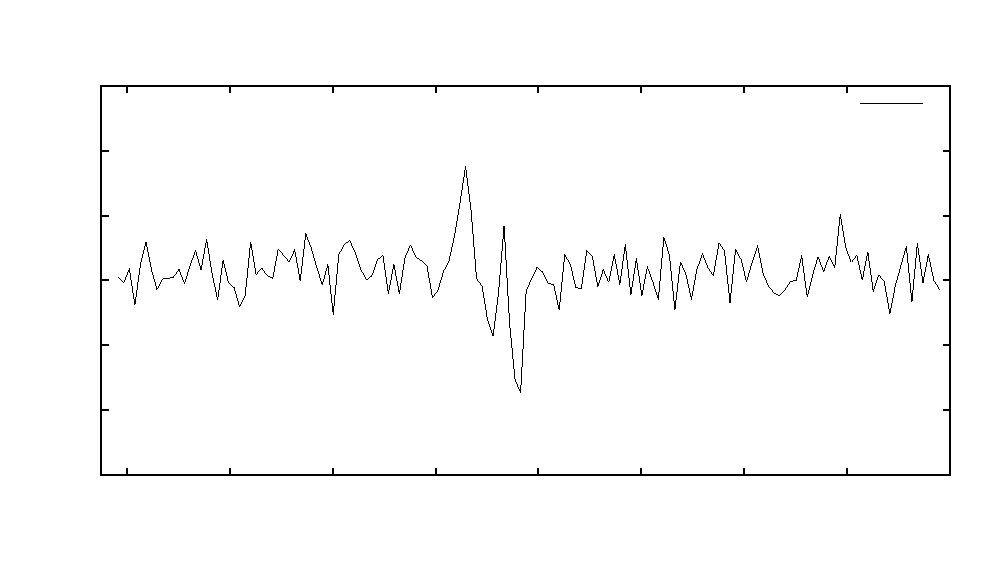
\includegraphics{ma03-12}}%
    \gplfronttext
  \end{picture}%
\endgroup

			\caption{\centering Parameter: Modulationsspannung 2V, AQ 30s, Empfindlichkeit 1mV, Phase 0^\circ}
		\end{figure}

		\begin{figure}[H]
			\center
			% GNUPLOT: LaTeX picture with Postscript
\begingroup
  \makeatletter
  \providecommand\color[2][]{%
    \GenericError{(gnuplot) \space\space\space\@spaces}{%
      Package color not loaded in conjunction with
      terminal option `colourtext'%
    }{See the gnuplot documentation for explanation.%
    }{Either use 'blacktext' in gnuplot or load the package
      color.sty in LaTeX.}%
    \renewcommand\color[2][]{}%
  }%
  \providecommand\includegraphics[2][]{%
    \GenericError{(gnuplot) \space\space\space\@spaces}{%
      Package graphicx or graphics not loaded%
    }{See the gnuplot documentation for explanation.%
    }{The gnuplot epslatex terminal needs graphicx.sty or graphics.sty.}%
    \renewcommand\includegraphics[2][]{}%
  }%
  \providecommand\rotatebox[2]{#2}%
  \@ifundefined{ifGPcolor}{%
    \newif\ifGPcolor
    \GPcolorfalse
  }{}%
  \@ifundefined{ifGPblacktext}{%
    \newif\ifGPblacktext
    \GPblacktexttrue
  }{}%
  % define a \g@addto@macro without @ in the name:
  \let\gplgaddtomacro\g@addto@macro
  % define empty templates for all commands taking text:
  \gdef\gplbacktext{}%
  \gdef\gplfronttext{}%
  \makeatother
  \ifGPblacktext
    % no textcolor at all
    \def\colorrgb#1{}%
    \def\colorgray#1{}%
  \else
    % gray or color?
    \ifGPcolor
      \def\colorrgb#1{\color[rgb]{#1}}%
      \def\colorgray#1{\color[gray]{#1}}%
      \expandafter\def\csname LTw\endcsname{\color{white}}%
      \expandafter\def\csname LTb\endcsname{\color{black}}%
      \expandafter\def\csname LTa\endcsname{\color{black}}%
      \expandafter\def\csname LT0\endcsname{\color[rgb]{1,0,0}}%
      \expandafter\def\csname LT1\endcsname{\color[rgb]{0,1,0}}%
      \expandafter\def\csname LT2\endcsname{\color[rgb]{0,0,1}}%
      \expandafter\def\csname LT3\endcsname{\color[rgb]{1,0,1}}%
      \expandafter\def\csname LT4\endcsname{\color[rgb]{0,1,1}}%
      \expandafter\def\csname LT5\endcsname{\color[rgb]{1,1,0}}%
      \expandafter\def\csname LT6\endcsname{\color[rgb]{0,0,0}}%
      \expandafter\def\csname LT7\endcsname{\color[rgb]{1,0.3,0}}%
      \expandafter\def\csname LT8\endcsname{\color[rgb]{0.5,0.5,0.5}}%
    \else
      % gray
      \def\colorrgb#1{\color{black}}%
      \def\colorgray#1{\color[gray]{#1}}%
      \expandafter\def\csname LTw\endcsname{\color{white}}%
      \expandafter\def\csname LTb\endcsname{\color{black}}%
      \expandafter\def\csname LTa\endcsname{\color{black}}%
      \expandafter\def\csname LT0\endcsname{\color{black}}%
      \expandafter\def\csname LT1\endcsname{\color{black}}%
      \expandafter\def\csname LT2\endcsname{\color{black}}%
      \expandafter\def\csname LT3\endcsname{\color{black}}%
      \expandafter\def\csname LT4\endcsname{\color{black}}%
      \expandafter\def\csname LT5\endcsname{\color{black}}%
      \expandafter\def\csname LT6\endcsname{\color{black}}%
      \expandafter\def\csname LT7\endcsname{\color{black}}%
      \expandafter\def\csname LT8\endcsname{\color{black}}%
    \fi
  \fi
  \setlength{\unitlength}{0.0500bp}%
  \begin{picture}(9354.00,5102.00)%
    \gplgaddtomacro\gplbacktext{%
      \csname LTb\endcsname%
      \put(682,704){\makebox(0,0)[r]{\strut{}-3}}%
      \put(682,1327){\makebox(0,0)[r]{\strut{}-2}}%
      \put(682,1950){\makebox(0,0)[r]{\strut{}-1}}%
      \put(682,2573){\makebox(0,0)[r]{\strut{} 0}}%
      \put(682,3195){\makebox(0,0)[r]{\strut{} 1}}%
      \put(682,3818){\makebox(0,0)[r]{\strut{} 2}}%
      \put(682,4441){\makebox(0,0)[r]{\strut{} 3}}%
      \put(1061,484){\makebox(0,0){\strut{} 280}}%
      \put(2048,484){\makebox(0,0){\strut{} 300}}%
      \put(3035,484){\makebox(0,0){\strut{} 320}}%
      \put(4022,484){\makebox(0,0){\strut{} 340}}%
      \put(5009,484){\makebox(0,0){\strut{} 360}}%
      \put(5996,484){\makebox(0,0){\strut{} 380}}%
      \put(6983,484){\makebox(0,0){\strut{} 400}}%
      \put(7970,484){\makebox(0,0){\strut{} 420}}%
      \put(8957,484){\makebox(0,0){\strut{} 440}}%
      \put(176,2572){\rotatebox{-270}{\makebox(0,0){\strut{}$dN/dE \ [1]$}}}%
      \put(4885,154){\makebox(0,0){\strut{}$E \ [eV]$}}%
      \put(4885,4771){\makebox(0,0){\strut{}Ag-Spektrum mit Zeitkonstante $300ms$}}%
    }%
    \gplgaddtomacro\gplfronttext{%
      \csname LTb\endcsname%
      \put(7970,4268){\makebox(0,0)[r]{\strut{}Messwerte}}%
    }%
    \gplbacktext
    \put(0,0){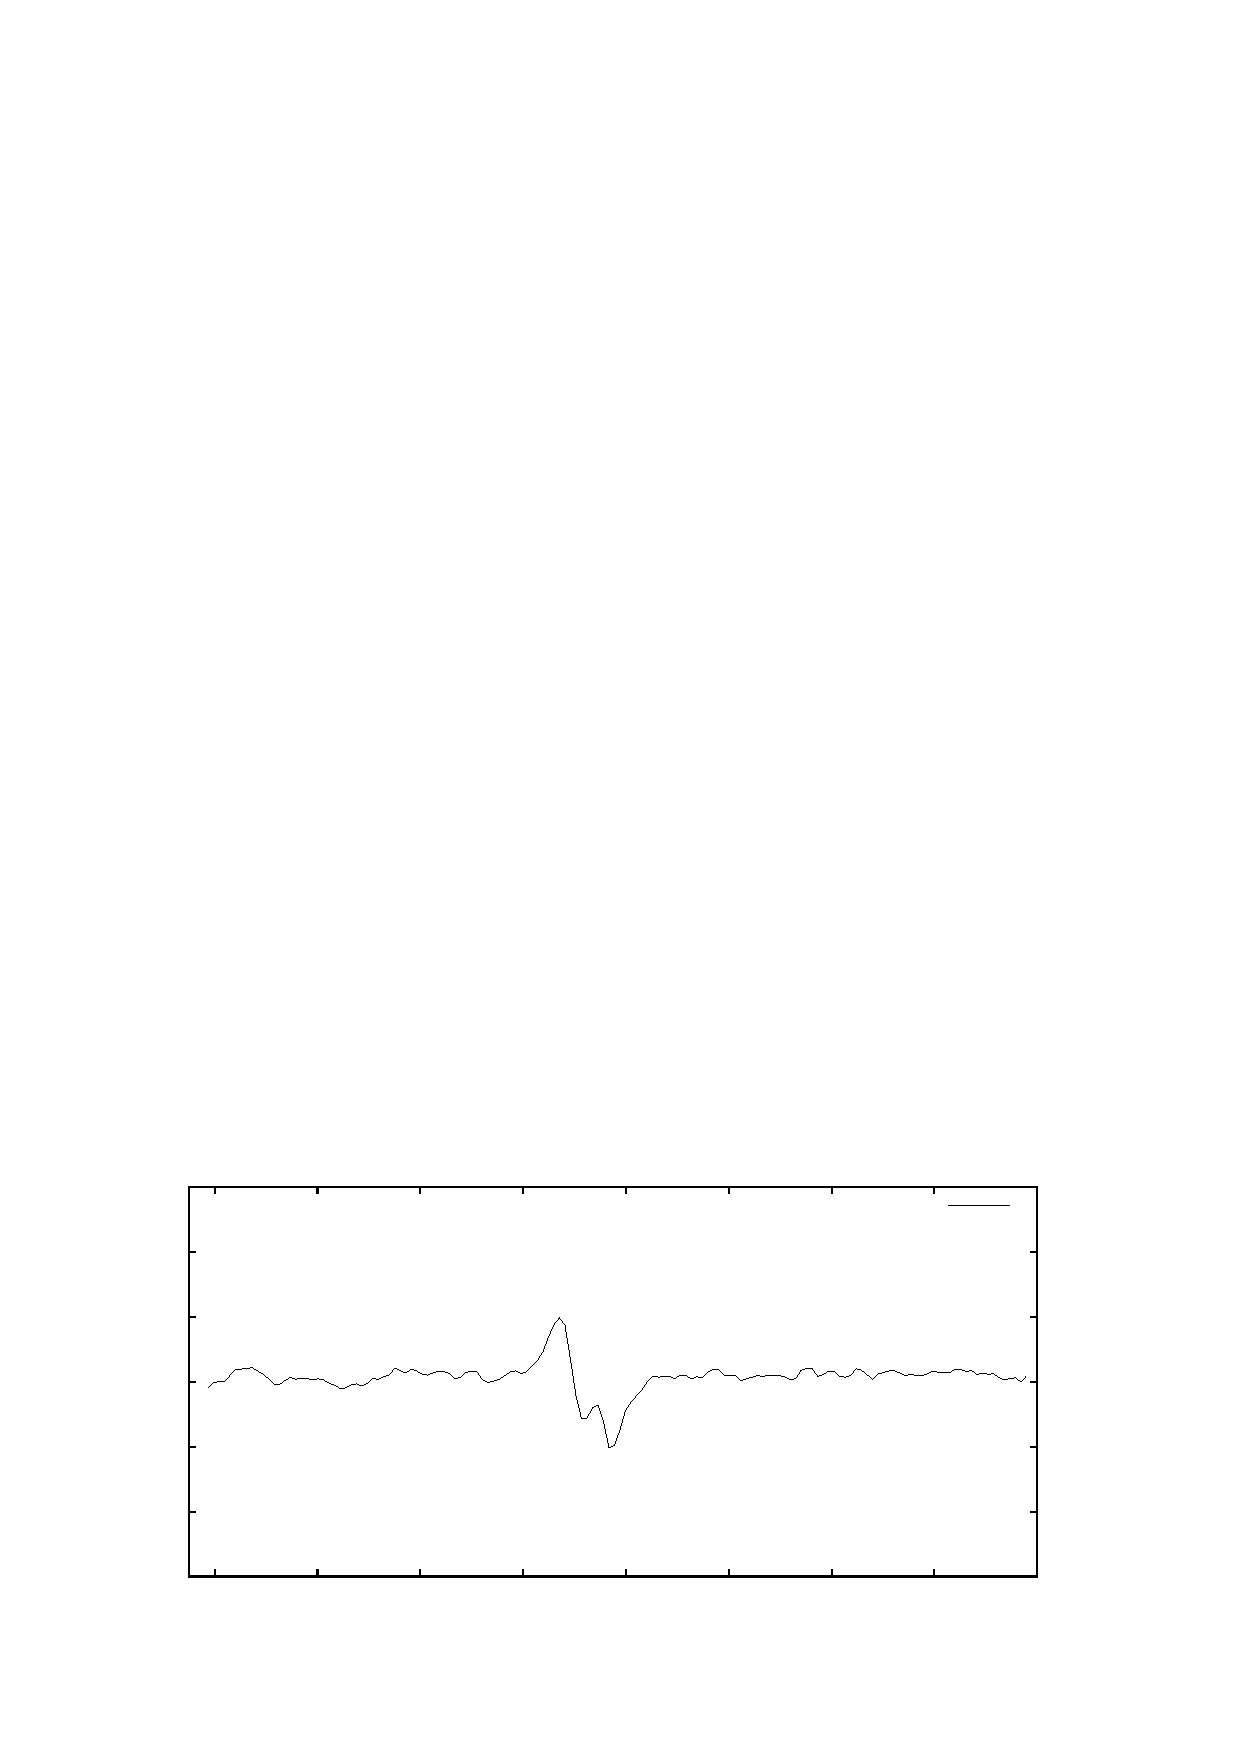
\includegraphics{ma03-11}}%
    \gplfronttext
  \end{picture}%
\endgroup

			\caption{\centering Parameter: Modulationsspannung 2V, AQ 30s, Empfindlichkeit 1mV, Phase 0^\circ}
		\end{figure}

		\begin{figure}[H]
			\center
			% GNUPLOT: LaTeX picture with Postscript
\begingroup
  \makeatletter
  \providecommand\color[2][]{%
    \GenericError{(gnuplot) \space\space\space\@spaces}{%
      Package color not loaded in conjunction with
      terminal option `colourtext'%
    }{See the gnuplot documentation for explanation.%
    }{Either use 'blacktext' in gnuplot or load the package
      color.sty in LaTeX.}%
    \renewcommand\color[2][]{}%
  }%
  \providecommand\includegraphics[2][]{%
    \GenericError{(gnuplot) \space\space\space\@spaces}{%
      Package graphicx or graphics not loaded%
    }{See the gnuplot documentation for explanation.%
    }{The gnuplot epslatex terminal needs graphicx.sty or graphics.sty.}%
    \renewcommand\includegraphics[2][]{}%
  }%
  \providecommand\rotatebox[2]{#2}%
  \@ifundefined{ifGPcolor}{%
    \newif\ifGPcolor
    \GPcolorfalse
  }{}%
  \@ifundefined{ifGPblacktext}{%
    \newif\ifGPblacktext
    \GPblacktexttrue
  }{}%
  % define a \g@addto@macro without @ in the name:
  \let\gplgaddtomacro\g@addto@macro
  % define empty templates for all commands taking text:
  \gdef\gplbacktext{}%
  \gdef\gplfronttext{}%
  \makeatother
  \ifGPblacktext
    % no textcolor at all
    \def\colorrgb#1{}%
    \def\colorgray#1{}%
  \else
    % gray or color?
    \ifGPcolor
      \def\colorrgb#1{\color[rgb]{#1}}%
      \def\colorgray#1{\color[gray]{#1}}%
      \expandafter\def\csname LTw\endcsname{\color{white}}%
      \expandafter\def\csname LTb\endcsname{\color{black}}%
      \expandafter\def\csname LTa\endcsname{\color{black}}%
      \expandafter\def\csname LT0\endcsname{\color[rgb]{1,0,0}}%
      \expandafter\def\csname LT1\endcsname{\color[rgb]{0,1,0}}%
      \expandafter\def\csname LT2\endcsname{\color[rgb]{0,0,1}}%
      \expandafter\def\csname LT3\endcsname{\color[rgb]{1,0,1}}%
      \expandafter\def\csname LT4\endcsname{\color[rgb]{0,1,1}}%
      \expandafter\def\csname LT5\endcsname{\color[rgb]{1,1,0}}%
      \expandafter\def\csname LT6\endcsname{\color[rgb]{0,0,0}}%
      \expandafter\def\csname LT7\endcsname{\color[rgb]{1,0.3,0}}%
      \expandafter\def\csname LT8\endcsname{\color[rgb]{0.5,0.5,0.5}}%
    \else
      % gray
      \def\colorrgb#1{\color{black}}%
      \def\colorgray#1{\color[gray]{#1}}%
      \expandafter\def\csname LTw\endcsname{\color{white}}%
      \expandafter\def\csname LTb\endcsname{\color{black}}%
      \expandafter\def\csname LTa\endcsname{\color{black}}%
      \expandafter\def\csname LT0\endcsname{\color{black}}%
      \expandafter\def\csname LT1\endcsname{\color{black}}%
      \expandafter\def\csname LT2\endcsname{\color{black}}%
      \expandafter\def\csname LT3\endcsname{\color{black}}%
      \expandafter\def\csname LT4\endcsname{\color{black}}%
      \expandafter\def\csname LT5\endcsname{\color{black}}%
      \expandafter\def\csname LT6\endcsname{\color{black}}%
      \expandafter\def\csname LT7\endcsname{\color{black}}%
      \expandafter\def\csname LT8\endcsname{\color{black}}%
    \fi
  \fi
  \setlength{\unitlength}{0.0500bp}%
  \begin{picture}(9354.00,5102.00)%
    \gplgaddtomacro\gplbacktext{%
      \csname LTb\endcsname%
      \put(682,704){\makebox(0,0)[r]{\strut{}-3}}%
      \put(682,1327){\makebox(0,0)[r]{\strut{}-2}}%
      \put(682,1950){\makebox(0,0)[r]{\strut{}-1}}%
      \put(682,2573){\makebox(0,0)[r]{\strut{} 0}}%
      \put(682,3195){\makebox(0,0)[r]{\strut{} 1}}%
      \put(682,3818){\makebox(0,0)[r]{\strut{} 2}}%
      \put(682,4441){\makebox(0,0)[r]{\strut{} 3}}%
      \put(1061,484){\makebox(0,0){\strut{} 280}}%
      \put(2048,484){\makebox(0,0){\strut{} 300}}%
      \put(3035,484){\makebox(0,0){\strut{} 320}}%
      \put(4022,484){\makebox(0,0){\strut{} 340}}%
      \put(5009,484){\makebox(0,0){\strut{} 360}}%
      \put(5996,484){\makebox(0,0){\strut{} 380}}%
      \put(6983,484){\makebox(0,0){\strut{} 400}}%
      \put(7970,484){\makebox(0,0){\strut{} 420}}%
      \put(8957,484){\makebox(0,0){\strut{} 440}}%
      \put(176,2572){\rotatebox{-270}{\makebox(0,0){\strut{}$dN/dE \ [1]$}}}%
      \put(4885,154){\makebox(0,0){\strut{}$E \ [eV]$}}%
      \put(4885,4771){\makebox(0,0){\strut{}Ag-Spektrum mit Zeitkonstante $1000ms$}}%
    }%
    \gplgaddtomacro\gplfronttext{%
      \csname LTb\endcsname%
      \put(7970,4268){\makebox(0,0)[r]{\strut{}Messwerte}}%
    }%
    \gplbacktext
    \put(0,0){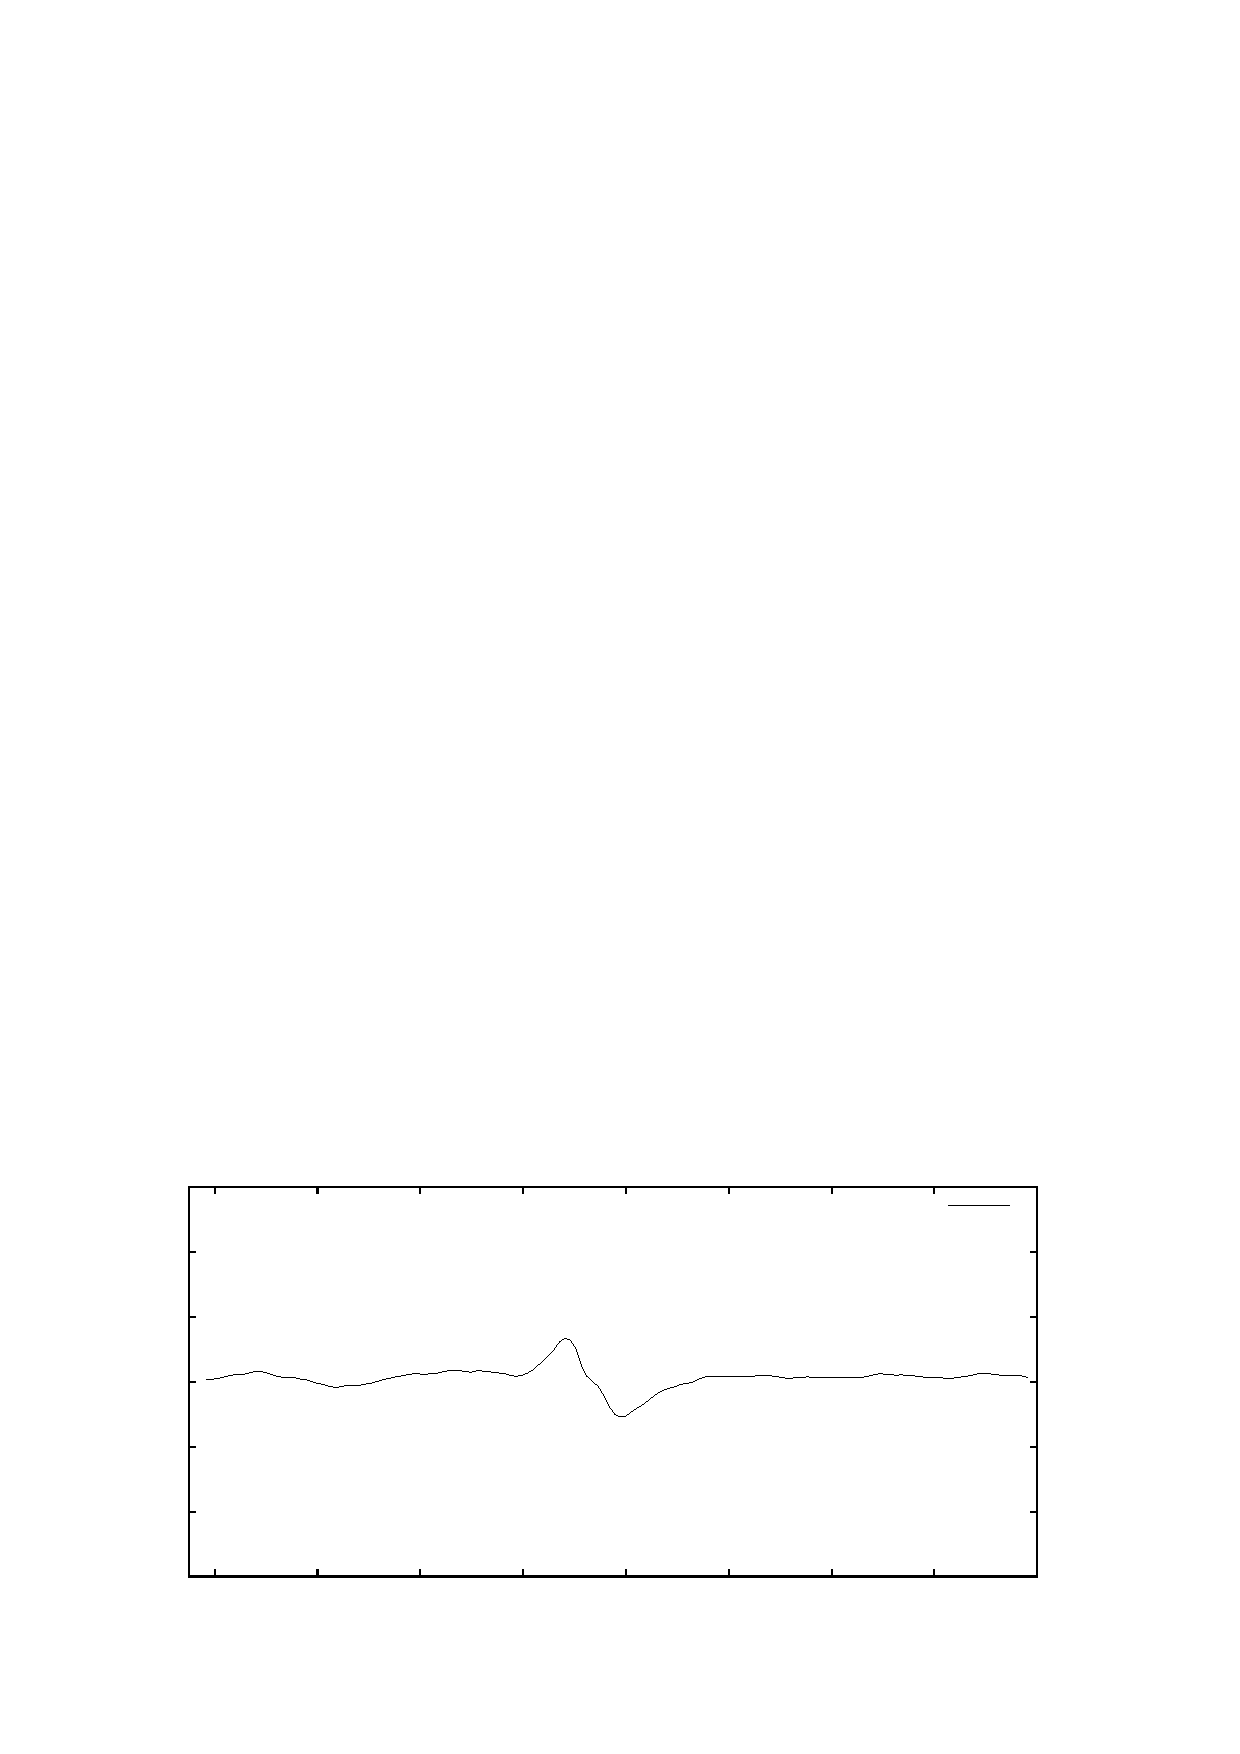
\includegraphics{ma03-10}}%
    \gplfronttext
  \end{picture}%
\endgroup

			\caption{\centering Parameter: Modulationsspannung 2V, AQ 30s, Empfindlichkeit 1mV, Phase 0^\circ}
		\end{figure}

		Es ist nun erkennbar, dass durch die zeitliche Mittelung ein besseres Signal-Rausch-Verhältnis erlangt werden kann.
		Wählt man die Zeitkonstante jedoch zu groß, so wird das Auflösungsvermögen drastisch verringert. Eine einfache Rechnung zeigt, über wie viel Elektronenvolt gemittelt wird:

		\begin{equation*}
			\Delta E = \dfrac{\Delta U_{CMA} \cdot K \cdot \text{\itshape Zeitkonstante}}{\text{\itshape Aquirationtime}}
		\end{equation*}
	

		Spannungsbereich und Aquirationtime wurden bei den drei Aufnahmen nicht verändert.
		\begin{equation*}
			\dfrac{\Delta U_{CMA} \cdot K}{\text{\itshape Aquirationtime}} = \dfrac{200V \cdot 1.624}{30s} \approx 10.8 \dfrac{V}{s}
		\end{equation*}
		\begin{itemize}
			\item 
				$10.8 Vs^{-1} \cdot 10ms = 108mV$
			\item 
				$10.8 Vs^{-1} \cdot 300ms = 3.25V$
			\item 
				$10.8 Vs^{-1} \cdot 1000ms = 10.8V$
		\end{itemize}
		Demnach ist es auch plausibel, dass der Doppelpeak bei 10 und 300ms Zeitkonstante noch zu erkennen war, wogegen er bei 1000ms verschwimmt.

	% subsubsection zeitkonstante (end)

	\subsubsection{Phase} % (fold)
	\label{ssub:phase}
	
		\begin{figure}[H]
			\center
			% GNUPLOT: LaTeX picture with Postscript
\begingroup
  \makeatletter
  \providecommand\color[2][]{%
    \GenericError{(gnuplot) \space\space\space\@spaces}{%
      Package color not loaded in conjunction with
      terminal option `colourtext'%
    }{See the gnuplot documentation for explanation.%
    }{Either use 'blacktext' in gnuplot or load the package
      color.sty in LaTeX.}%
    \renewcommand\color[2][]{}%
  }%
  \providecommand\includegraphics[2][]{%
    \GenericError{(gnuplot) \space\space\space\@spaces}{%
      Package graphicx or graphics not loaded%
    }{See the gnuplot documentation for explanation.%
    }{The gnuplot epslatex terminal needs graphicx.sty or graphics.sty.}%
    \renewcommand\includegraphics[2][]{}%
  }%
  \providecommand\rotatebox[2]{#2}%
  \@ifundefined{ifGPcolor}{%
    \newif\ifGPcolor
    \GPcolorfalse
  }{}%
  \@ifundefined{ifGPblacktext}{%
    \newif\ifGPblacktext
    \GPblacktexttrue
  }{}%
  % define a \g@addto@macro without @ in the name:
  \let\gplgaddtomacro\g@addto@macro
  % define empty templates for all commands taking text:
  \gdef\gplbacktext{}%
  \gdef\gplfronttext{}%
  \makeatother
  \ifGPblacktext
    % no textcolor at all
    \def\colorrgb#1{}%
    \def\colorgray#1{}%
  \else
    % gray or color?
    \ifGPcolor
      \def\colorrgb#1{\color[rgb]{#1}}%
      \def\colorgray#1{\color[gray]{#1}}%
      \expandafter\def\csname LTw\endcsname{\color{white}}%
      \expandafter\def\csname LTb\endcsname{\color{black}}%
      \expandafter\def\csname LTa\endcsname{\color{black}}%
      \expandafter\def\csname LT0\endcsname{\color[rgb]{1,0,0}}%
      \expandafter\def\csname LT1\endcsname{\color[rgb]{0,1,0}}%
      \expandafter\def\csname LT2\endcsname{\color[rgb]{0,0,1}}%
      \expandafter\def\csname LT3\endcsname{\color[rgb]{1,0,1}}%
      \expandafter\def\csname LT4\endcsname{\color[rgb]{0,1,1}}%
      \expandafter\def\csname LT5\endcsname{\color[rgb]{1,1,0}}%
      \expandafter\def\csname LT6\endcsname{\color[rgb]{0,0,0}}%
      \expandafter\def\csname LT7\endcsname{\color[rgb]{1,0.3,0}}%
      \expandafter\def\csname LT8\endcsname{\color[rgb]{0.5,0.5,0.5}}%
    \else
      % gray
      \def\colorrgb#1{\color{black}}%
      \def\colorgray#1{\color[gray]{#1}}%
      \expandafter\def\csname LTw\endcsname{\color{white}}%
      \expandafter\def\csname LTb\endcsname{\color{black}}%
      \expandafter\def\csname LTa\endcsname{\color{black}}%
      \expandafter\def\csname LT0\endcsname{\color{black}}%
      \expandafter\def\csname LT1\endcsname{\color{black}}%
      \expandafter\def\csname LT2\endcsname{\color{black}}%
      \expandafter\def\csname LT3\endcsname{\color{black}}%
      \expandafter\def\csname LT4\endcsname{\color{black}}%
      \expandafter\def\csname LT5\endcsname{\color{black}}%
      \expandafter\def\csname LT6\endcsname{\color{black}}%
      \expandafter\def\csname LT7\endcsname{\color{black}}%
      \expandafter\def\csname LT8\endcsname{\color{black}}%
    \fi
  \fi
  \setlength{\unitlength}{0.0500bp}%
  \begin{picture}(9354.00,5102.00)%
    \gplgaddtomacro\gplbacktext{%
      \csname LTb\endcsname%
      \put(946,704){\makebox(0,0)[r]{\strut{}-2}}%
      \put(946,1171){\makebox(0,0)[r]{\strut{}-1.5}}%
      \put(946,1638){\makebox(0,0)[r]{\strut{}-1}}%
      \put(946,2105){\makebox(0,0)[r]{\strut{}-0.5}}%
      \put(946,2573){\makebox(0,0)[r]{\strut{} 0}}%
      \put(946,3040){\makebox(0,0)[r]{\strut{} 0.5}}%
      \put(946,3507){\makebox(0,0)[r]{\strut{} 1}}%
      \put(946,3974){\makebox(0,0)[r]{\strut{} 1.5}}%
      \put(946,4441){\makebox(0,0)[r]{\strut{} 2}}%
      \put(1078,484){\makebox(0,0){\strut{} 310}}%
      \put(1953,484){\makebox(0,0){\strut{} 320}}%
      \put(2829,484){\makebox(0,0){\strut{} 330}}%
      \put(3704,484){\makebox(0,0){\strut{} 340}}%
      \put(4580,484){\makebox(0,0){\strut{} 350}}%
      \put(5455,484){\makebox(0,0){\strut{} 360}}%
      \put(6331,484){\makebox(0,0){\strut{} 370}}%
      \put(7206,484){\makebox(0,0){\strut{} 380}}%
      \put(8082,484){\makebox(0,0){\strut{} 390}}%
      \put(8957,484){\makebox(0,0){\strut{} 400}}%
      \put(176,2572){\rotatebox{-270}{\makebox(0,0){\strut{}$dN/dE \ [1]$}}}%
      \put(5017,154){\makebox(0,0){\strut{}$E \ [eV]$}}%
      \put(5017,4771){\makebox(0,0){\strut{}Ag-Spektrum mit Phase $45^\circ$}}%
    }%
    \gplgaddtomacro\gplfronttext{%
      \csname LTb\endcsname%
      \put(7970,4268){\makebox(0,0)[r]{\strut{}Messwerte}}%
    }%
    \gplbacktext
    \put(0,0){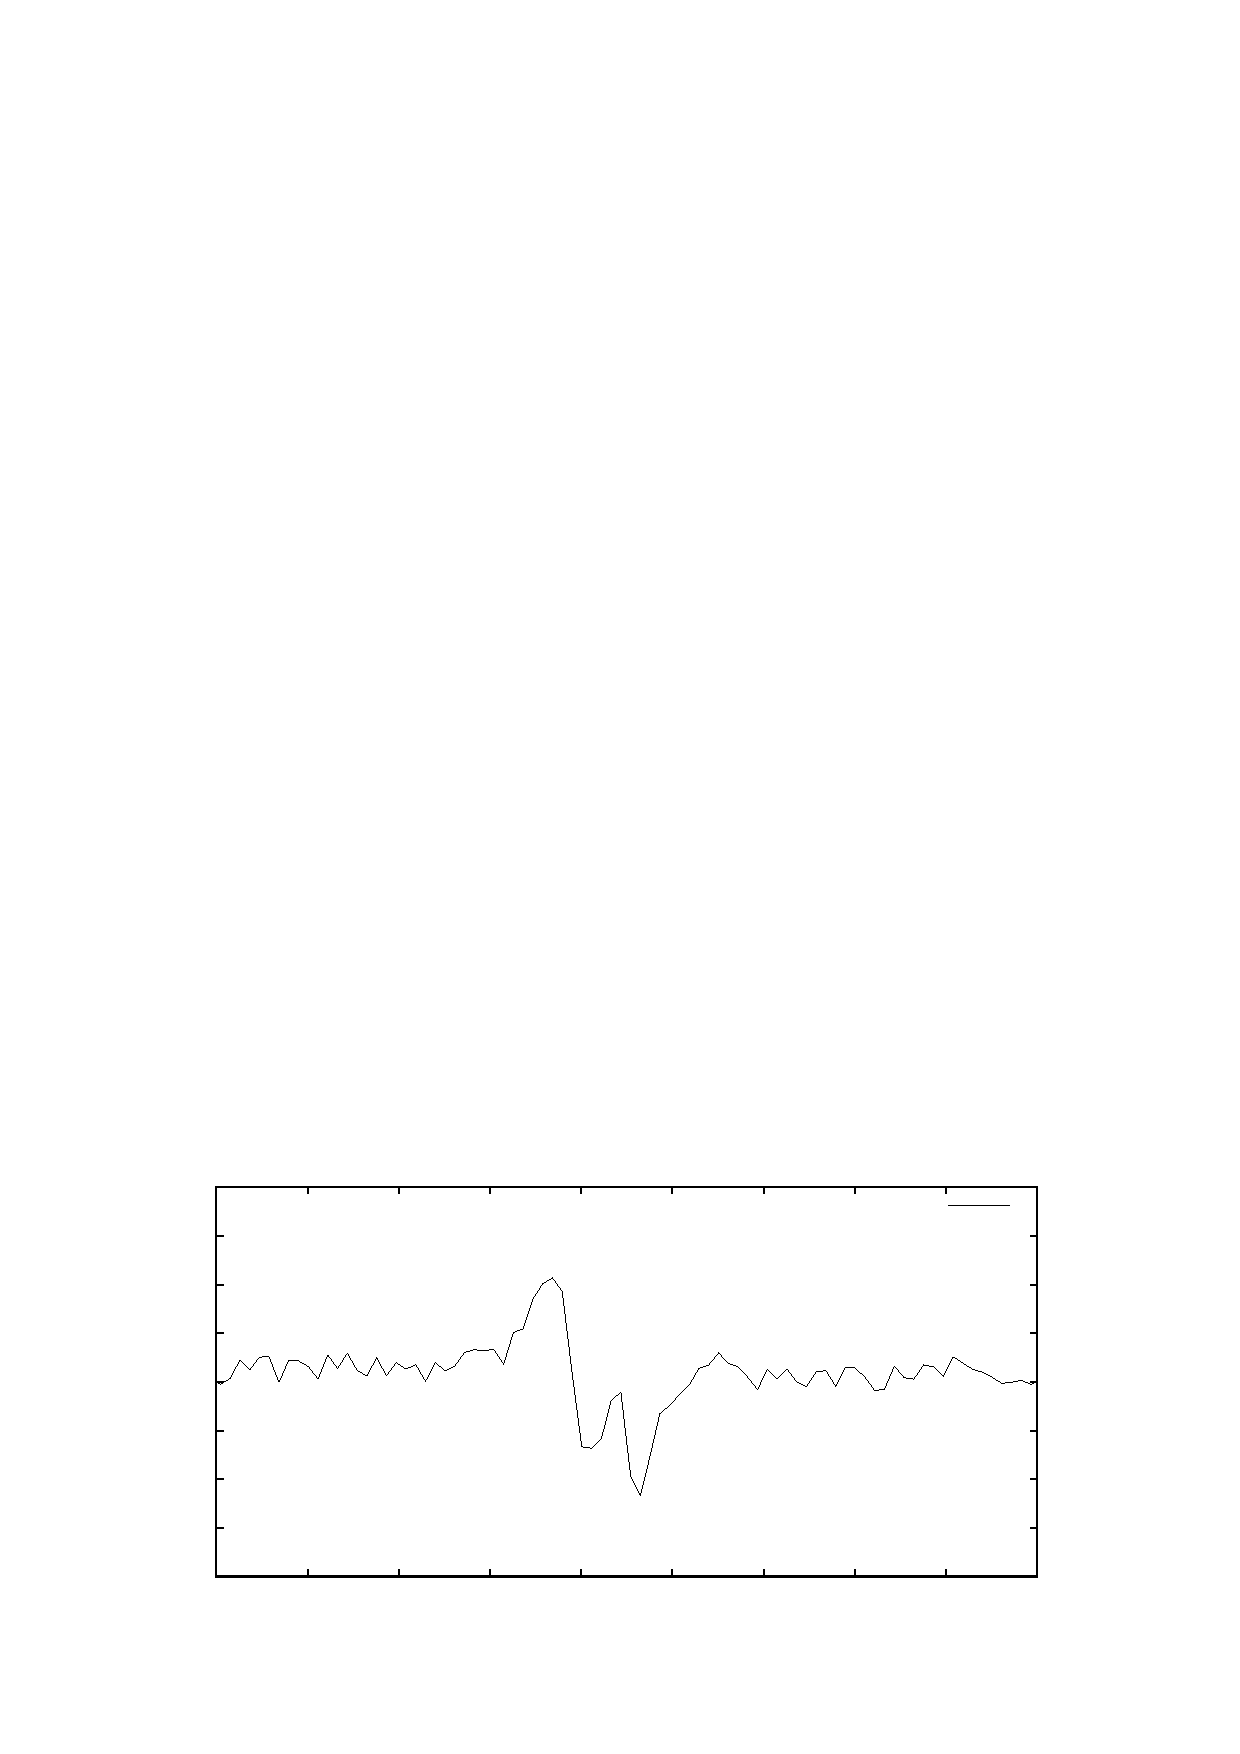
\includegraphics{ma03-08}}%
    \gplfronttext
  \end{picture}%
\endgroup

			\caption{\centering Parameter: Modulationsspannung 2V, AQ 30s, Empfindlichkeit 1mV, Zeitkonstante 100ms}
		\end{figure}

		\begin{figure}[H]
			\center
			% GNUPLOT: LaTeX picture with Postscript
\begingroup
  \makeatletter
  \providecommand\color[2][]{%
    \GenericError{(gnuplot) \space\space\space\@spaces}{%
      Package color not loaded in conjunction with
      terminal option `colourtext'%
    }{See the gnuplot documentation for explanation.%
    }{Either use 'blacktext' in gnuplot or load the package
      color.sty in LaTeX.}%
    \renewcommand\color[2][]{}%
  }%
  \providecommand\includegraphics[2][]{%
    \GenericError{(gnuplot) \space\space\space\@spaces}{%
      Package graphicx or graphics not loaded%
    }{See the gnuplot documentation for explanation.%
    }{The gnuplot epslatex terminal needs graphicx.sty or graphics.sty.}%
    \renewcommand\includegraphics[2][]{}%
  }%
  \providecommand\rotatebox[2]{#2}%
  \@ifundefined{ifGPcolor}{%
    \newif\ifGPcolor
    \GPcolorfalse
  }{}%
  \@ifundefined{ifGPblacktext}{%
    \newif\ifGPblacktext
    \GPblacktexttrue
  }{}%
  % define a \g@addto@macro without @ in the name:
  \let\gplgaddtomacro\g@addto@macro
  % define empty templates for all commands taking text:
  \gdef\gplbacktext{}%
  \gdef\gplfronttext{}%
  \makeatother
  \ifGPblacktext
    % no textcolor at all
    \def\colorrgb#1{}%
    \def\colorgray#1{}%
  \else
    % gray or color?
    \ifGPcolor
      \def\colorrgb#1{\color[rgb]{#1}}%
      \def\colorgray#1{\color[gray]{#1}}%
      \expandafter\def\csname LTw\endcsname{\color{white}}%
      \expandafter\def\csname LTb\endcsname{\color{black}}%
      \expandafter\def\csname LTa\endcsname{\color{black}}%
      \expandafter\def\csname LT0\endcsname{\color[rgb]{1,0,0}}%
      \expandafter\def\csname LT1\endcsname{\color[rgb]{0,1,0}}%
      \expandafter\def\csname LT2\endcsname{\color[rgb]{0,0,1}}%
      \expandafter\def\csname LT3\endcsname{\color[rgb]{1,0,1}}%
      \expandafter\def\csname LT4\endcsname{\color[rgb]{0,1,1}}%
      \expandafter\def\csname LT5\endcsname{\color[rgb]{1,1,0}}%
      \expandafter\def\csname LT6\endcsname{\color[rgb]{0,0,0}}%
      \expandafter\def\csname LT7\endcsname{\color[rgb]{1,0.3,0}}%
      \expandafter\def\csname LT8\endcsname{\color[rgb]{0.5,0.5,0.5}}%
    \else
      % gray
      \def\colorrgb#1{\color{black}}%
      \def\colorgray#1{\color[gray]{#1}}%
      \expandafter\def\csname LTw\endcsname{\color{white}}%
      \expandafter\def\csname LTb\endcsname{\color{black}}%
      \expandafter\def\csname LTa\endcsname{\color{black}}%
      \expandafter\def\csname LT0\endcsname{\color{black}}%
      \expandafter\def\csname LT1\endcsname{\color{black}}%
      \expandafter\def\csname LT2\endcsname{\color{black}}%
      \expandafter\def\csname LT3\endcsname{\color{black}}%
      \expandafter\def\csname LT4\endcsname{\color{black}}%
      \expandafter\def\csname LT5\endcsname{\color{black}}%
      \expandafter\def\csname LT6\endcsname{\color{black}}%
      \expandafter\def\csname LT7\endcsname{\color{black}}%
      \expandafter\def\csname LT8\endcsname{\color{black}}%
    \fi
  \fi
  \setlength{\unitlength}{0.0500bp}%
  \begin{picture}(9354.00,5102.00)%
    \gplgaddtomacro\gplbacktext{%
      \csname LTb\endcsname%
      \put(946,704){\makebox(0,0)[r]{\strut{}-2}}%
      \put(946,1171){\makebox(0,0)[r]{\strut{}-1.5}}%
      \put(946,1638){\makebox(0,0)[r]{\strut{}-1}}%
      \put(946,2105){\makebox(0,0)[r]{\strut{}-0.5}}%
      \put(946,2573){\makebox(0,0)[r]{\strut{} 0}}%
      \put(946,3040){\makebox(0,0)[r]{\strut{} 0.5}}%
      \put(946,3507){\makebox(0,0)[r]{\strut{} 1}}%
      \put(946,3974){\makebox(0,0)[r]{\strut{} 1.5}}%
      \put(946,4441){\makebox(0,0)[r]{\strut{} 2}}%
      \put(1078,484){\makebox(0,0){\strut{} 310}}%
      \put(1953,484){\makebox(0,0){\strut{} 320}}%
      \put(2829,484){\makebox(0,0){\strut{} 330}}%
      \put(3704,484){\makebox(0,0){\strut{} 340}}%
      \put(4580,484){\makebox(0,0){\strut{} 350}}%
      \put(5455,484){\makebox(0,0){\strut{} 360}}%
      \put(6331,484){\makebox(0,0){\strut{} 370}}%
      \put(7206,484){\makebox(0,0){\strut{} 380}}%
      \put(8082,484){\makebox(0,0){\strut{} 390}}%
      \put(8957,484){\makebox(0,0){\strut{} 400}}%
      \put(176,2572){\rotatebox{-270}{\makebox(0,0){\strut{}$dN/dE \ [1]$}}}%
      \put(5017,154){\makebox(0,0){\strut{}$E \ [eV]$}}%
      \put(5017,4771){\makebox(0,0){\strut{}Ag-Spektrum mit Phase $180^\circ$}}%
    }%
    \gplgaddtomacro\gplfronttext{%
      \csname LTb\endcsname%
      \put(7970,4268){\makebox(0,0)[r]{\strut{}Messwerte}}%
    }%
    \gplbacktext
    \put(0,0){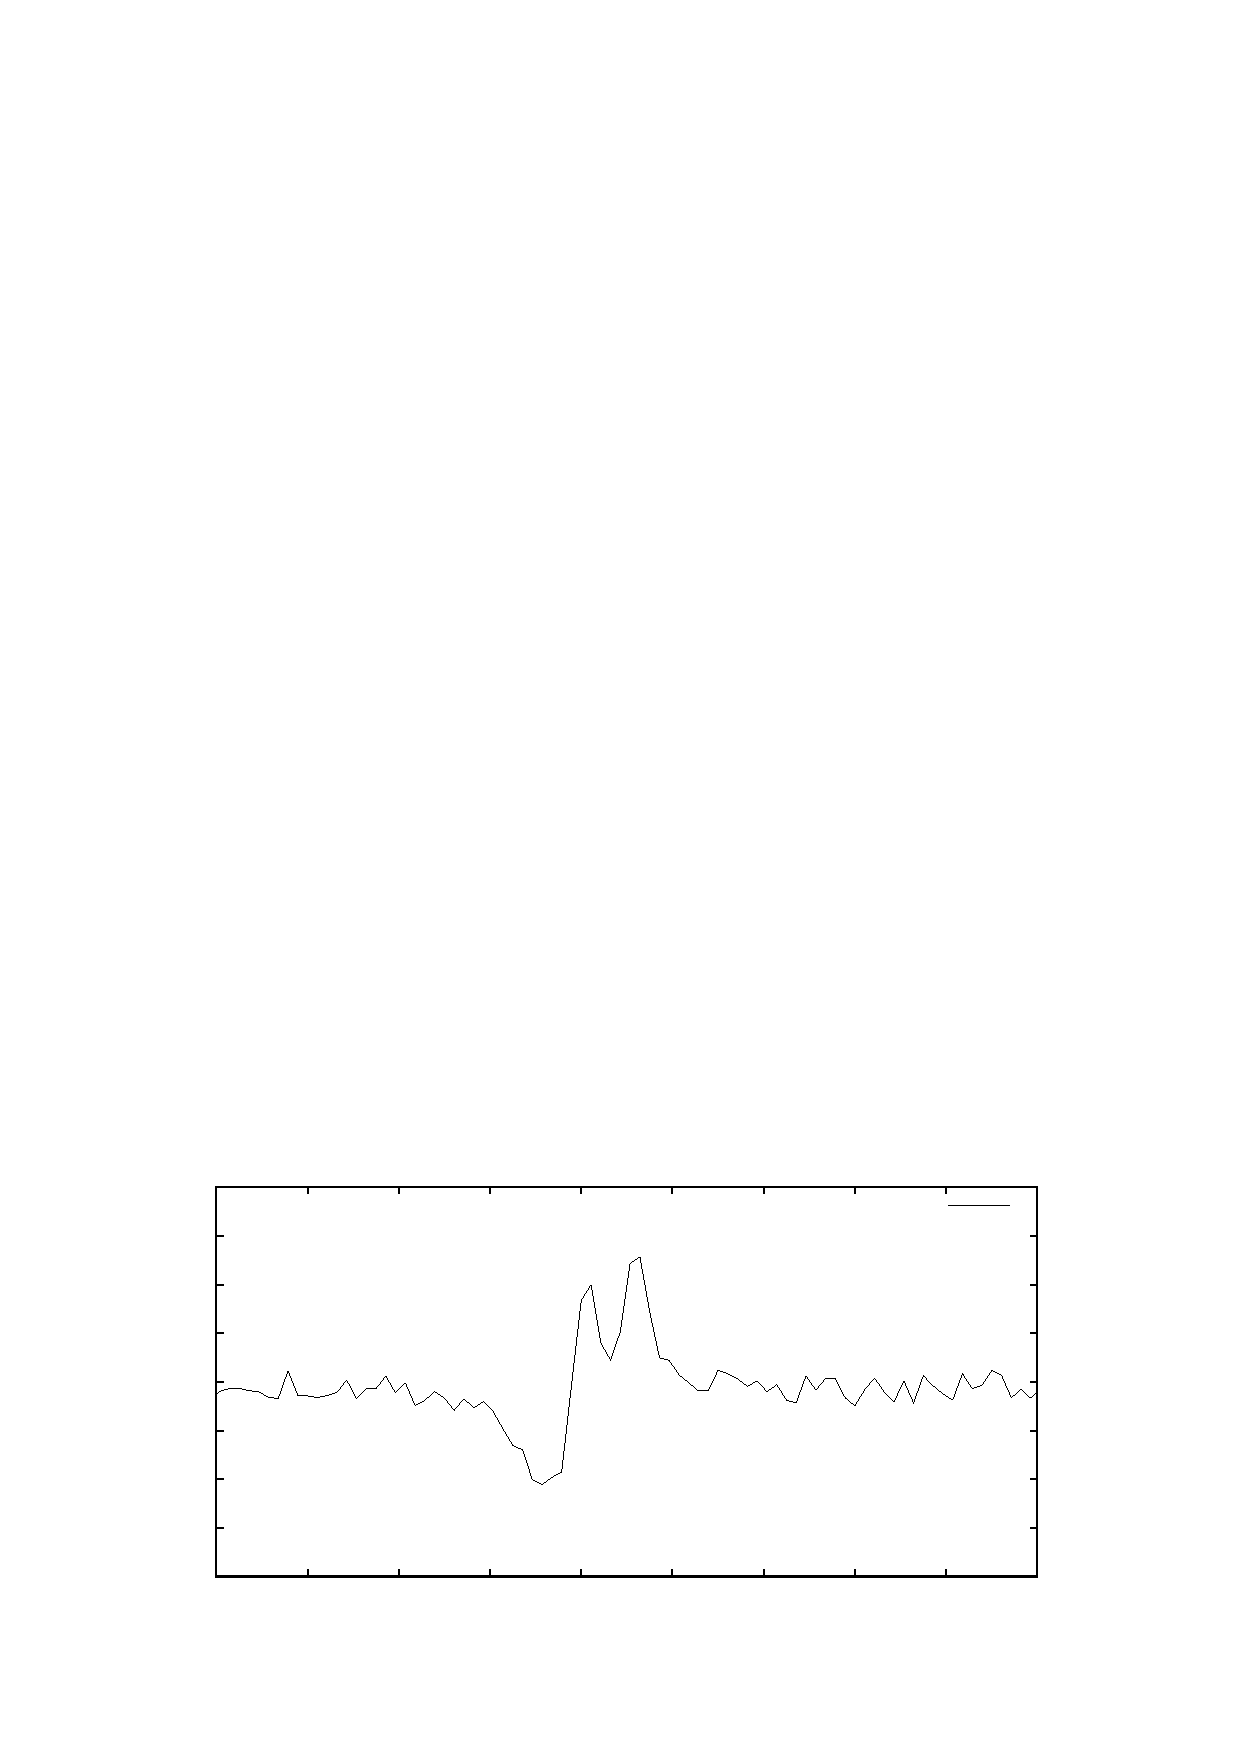
\includegraphics{ma03-07}}%
    \gplfronttext
  \end{picture}%
\endgroup

			\caption{\centering Parameter: Modulationsspannung 2V, AQ 30s, Empfindlichkeit 1mV, Zeitkonstante 100ms}
		\end{figure}

		\begin{figure}[H]
			\center
			% GNUPLOT: LaTeX picture with Postscript
\begingroup
  \makeatletter
  \providecommand\color[2][]{%
    \GenericError{(gnuplot) \space\space\space\@spaces}{%
      Package color not loaded in conjunction with
      terminal option `colourtext'%
    }{See the gnuplot documentation for explanation.%
    }{Either use 'blacktext' in gnuplot or load the package
      color.sty in LaTeX.}%
    \renewcommand\color[2][]{}%
  }%
  \providecommand\includegraphics[2][]{%
    \GenericError{(gnuplot) \space\space\space\@spaces}{%
      Package graphicx or graphics not loaded%
    }{See the gnuplot documentation for explanation.%
    }{The gnuplot epslatex terminal needs graphicx.sty or graphics.sty.}%
    \renewcommand\includegraphics[2][]{}%
  }%
  \providecommand\rotatebox[2]{#2}%
  \@ifundefined{ifGPcolor}{%
    \newif\ifGPcolor
    \GPcolorfalse
  }{}%
  \@ifundefined{ifGPblacktext}{%
    \newif\ifGPblacktext
    \GPblacktexttrue
  }{}%
  % define a \g@addto@macro without @ in the name:
  \let\gplgaddtomacro\g@addto@macro
  % define empty templates for all commands taking text:
  \gdef\gplbacktext{}%
  \gdef\gplfronttext{}%
  \makeatother
  \ifGPblacktext
    % no textcolor at all
    \def\colorrgb#1{}%
    \def\colorgray#1{}%
  \else
    % gray or color?
    \ifGPcolor
      \def\colorrgb#1{\color[rgb]{#1}}%
      \def\colorgray#1{\color[gray]{#1}}%
      \expandafter\def\csname LTw\endcsname{\color{white}}%
      \expandafter\def\csname LTb\endcsname{\color{black}}%
      \expandafter\def\csname LTa\endcsname{\color{black}}%
      \expandafter\def\csname LT0\endcsname{\color[rgb]{1,0,0}}%
      \expandafter\def\csname LT1\endcsname{\color[rgb]{0,1,0}}%
      \expandafter\def\csname LT2\endcsname{\color[rgb]{0,0,1}}%
      \expandafter\def\csname LT3\endcsname{\color[rgb]{1,0,1}}%
      \expandafter\def\csname LT4\endcsname{\color[rgb]{0,1,1}}%
      \expandafter\def\csname LT5\endcsname{\color[rgb]{1,1,0}}%
      \expandafter\def\csname LT6\endcsname{\color[rgb]{0,0,0}}%
      \expandafter\def\csname LT7\endcsname{\color[rgb]{1,0.3,0}}%
      \expandafter\def\csname LT8\endcsname{\color[rgb]{0.5,0.5,0.5}}%
    \else
      % gray
      \def\colorrgb#1{\color{black}}%
      \def\colorgray#1{\color[gray]{#1}}%
      \expandafter\def\csname LTw\endcsname{\color{white}}%
      \expandafter\def\csname LTb\endcsname{\color{black}}%
      \expandafter\def\csname LTa\endcsname{\color{black}}%
      \expandafter\def\csname LT0\endcsname{\color{black}}%
      \expandafter\def\csname LT1\endcsname{\color{black}}%
      \expandafter\def\csname LT2\endcsname{\color{black}}%
      \expandafter\def\csname LT3\endcsname{\color{black}}%
      \expandafter\def\csname LT4\endcsname{\color{black}}%
      \expandafter\def\csname LT5\endcsname{\color{black}}%
      \expandafter\def\csname LT6\endcsname{\color{black}}%
      \expandafter\def\csname LT7\endcsname{\color{black}}%
      \expandafter\def\csname LT8\endcsname{\color{black}}%
    \fi
  \fi
  \setlength{\unitlength}{0.0500bp}%
  \begin{picture}(9354.00,5102.00)%
    \gplgaddtomacro\gplbacktext{%
      \csname LTb\endcsname%
      \put(946,704){\makebox(0,0)[r]{\strut{}-2}}%
      \put(946,1171){\makebox(0,0)[r]{\strut{}-1.5}}%
      \put(946,1638){\makebox(0,0)[r]{\strut{}-1}}%
      \put(946,2105){\makebox(0,0)[r]{\strut{}-0.5}}%
      \put(946,2573){\makebox(0,0)[r]{\strut{} 0}}%
      \put(946,3040){\makebox(0,0)[r]{\strut{} 0.5}}%
      \put(946,3507){\makebox(0,0)[r]{\strut{} 1}}%
      \put(946,3974){\makebox(0,0)[r]{\strut{} 1.5}}%
      \put(946,4441){\makebox(0,0)[r]{\strut{} 2}}%
      \put(1078,484){\makebox(0,0){\strut{} 310}}%
      \put(1953,484){\makebox(0,0){\strut{} 320}}%
      \put(2829,484){\makebox(0,0){\strut{} 330}}%
      \put(3704,484){\makebox(0,0){\strut{} 340}}%
      \put(4580,484){\makebox(0,0){\strut{} 350}}%
      \put(5455,484){\makebox(0,0){\strut{} 360}}%
      \put(6331,484){\makebox(0,0){\strut{} 370}}%
      \put(7206,484){\makebox(0,0){\strut{} 380}}%
      \put(8082,484){\makebox(0,0){\strut{} 390}}%
      \put(8957,484){\makebox(0,0){\strut{} 400}}%
      \put(176,2572){\rotatebox{-270}{\makebox(0,0){\strut{}$dN/dE \ [1]$}}}%
      \put(5017,154){\makebox(0,0){\strut{}$E \ [eV]$}}%
      \put(5017,4771){\makebox(0,0){\strut{}Ag-Spektrum mit minimaler Phase bei $103^\circ$}}%
    }%
    \gplgaddtomacro\gplfronttext{%
      \csname LTb\endcsname%
      \put(7970,4268){\makebox(0,0)[r]{\strut{}Messwerte}}%
    }%
    \gplbacktext
    \put(0,0){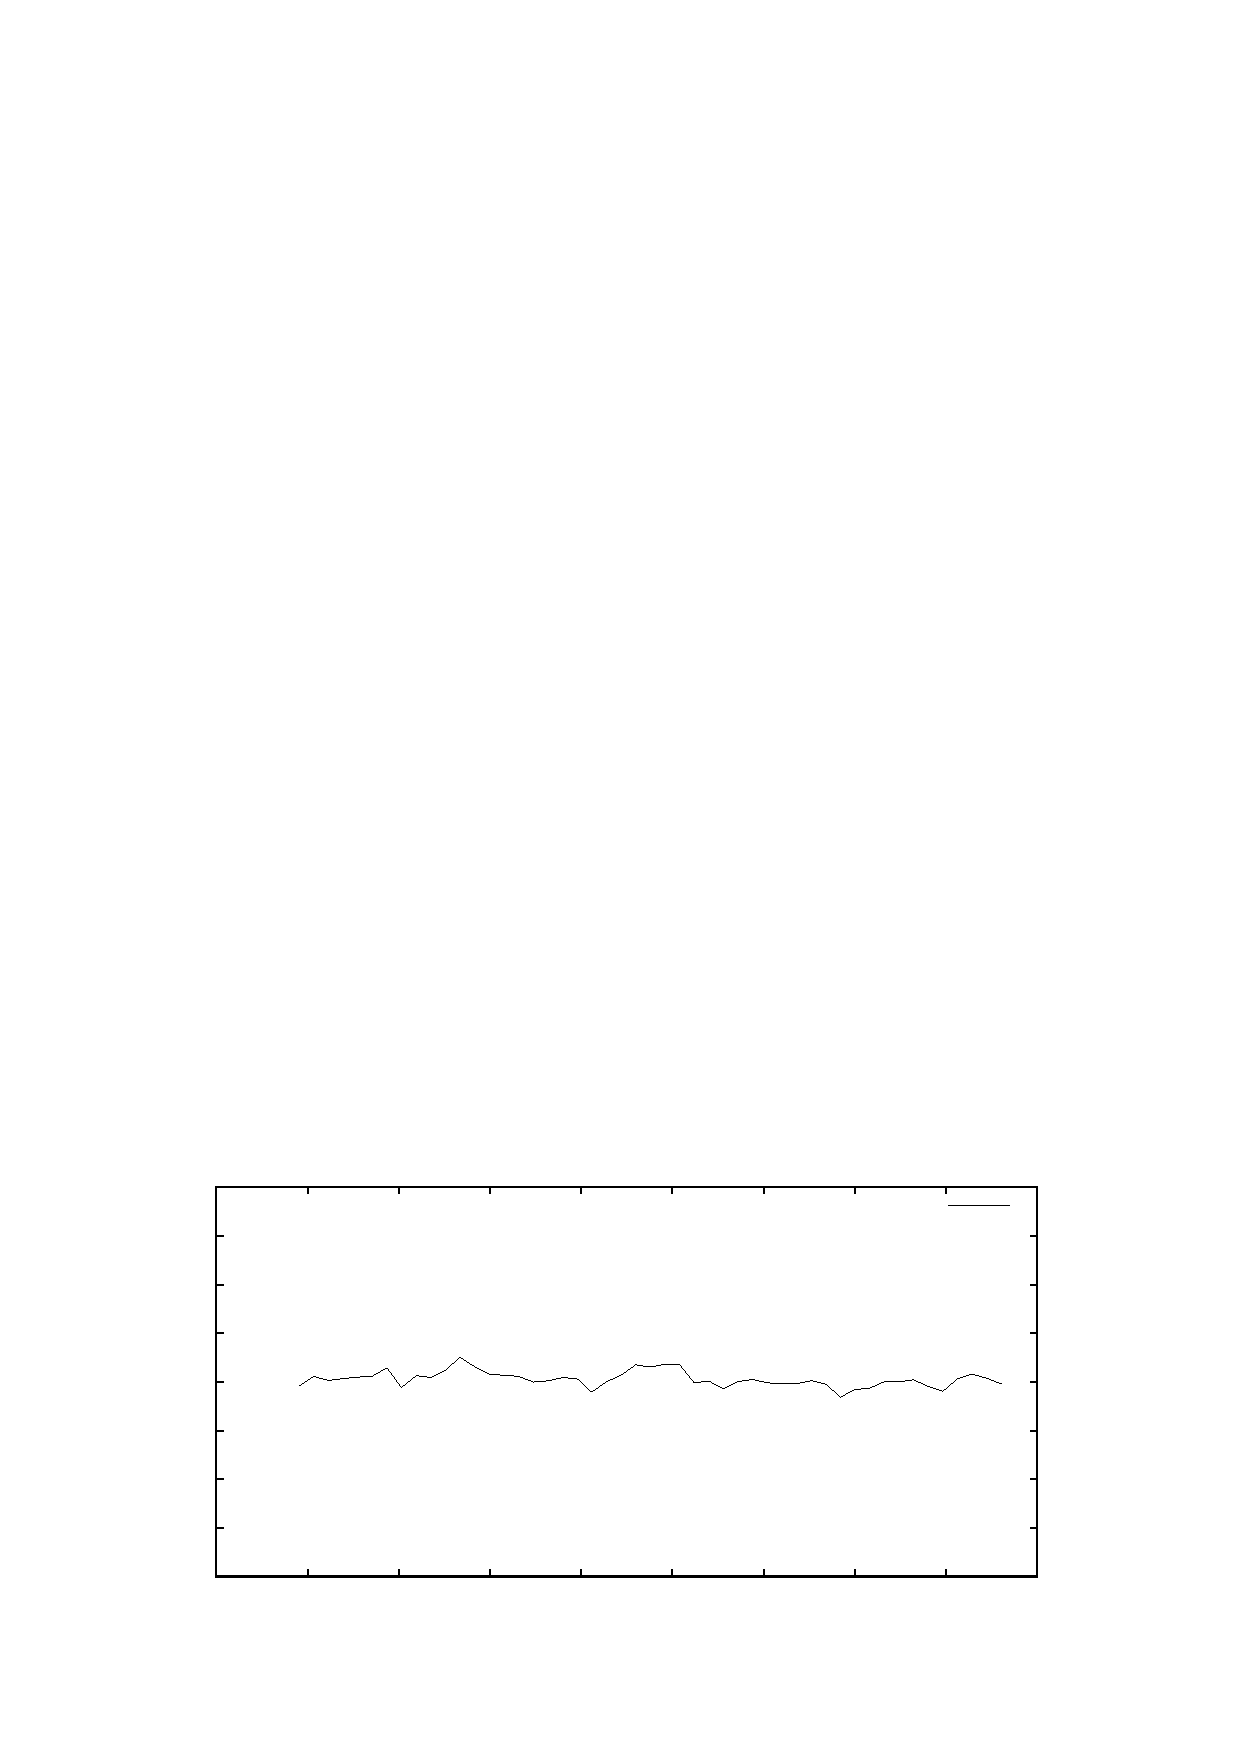
\includegraphics{ma03-14}}%
    \gplfronttext
  \end{picture}%
\endgroup

			\caption{\centering Parameter: Modulationsspannung 5V, AQ 10s, Empfindlichkeit 1mV, Zeitkonstante 300ms}
		\end{figure}

		Die Phasenverschiebung des Referenzsignals hat maßgeblich Einfluss auf die Amplitude des Signals, jedoch nicht oder kaum auf die Lage der Peaks. 
		Wie vermutet kehren sich bei einer Verschiebung in der Nähe von $180^\circ$ Minima und Maxima um. 
		Wenn man sich überlegt, wie zwei Sinusfunktionen im Demodulator multipliziert werden, so ergeben sie ohne Phasenverschiebung eine stets positive $\sin^2$-Funktion, mit einer Verschiebung von $180^\circ$ jedoch eine stets negative $–\sin^2$ Funktion. 
		Diese Überlegung macht den Vorzeichenwechsel plausibel. 
		Bei $103^\circ$ verschwand das Signal nahezu ganz. 
		Folglich muss der Phasenwinkel des maximalen Signals $90^\circ$ darunter liegen.
		Damit gilt also:
		\[
			\varphi_{max} = 13^\circ 
		\]
		Alle folgenden Spektren wurden mit einer Phasenverschiebung von $12^\circ$ aufgenommen.

	% subsubsection phase (end)

% subsection silber_spektrum (end)

\subsection{Analyse der Proben} % (fold)
\label{sub:qualitative_analyse_der_proben}

	\subsubsection{Probenhalter} % (fold)
	\label{ssub:probenhalter}
	
		\begin{figure}[H]
			\center
			% GNUPLOT: LaTeX picture with Postscript
\begingroup
  \makeatletter
  \providecommand\color[2][]{%
    \GenericError{(gnuplot) \space\space\space\@spaces}{%
      Package color not loaded in conjunction with
      terminal option `colourtext'%
    }{See the gnuplot documentation for explanation.%
    }{Either use 'blacktext' in gnuplot or load the package
      color.sty in LaTeX.}%
    \renewcommand\color[2][]{}%
  }%
  \providecommand\includegraphics[2][]{%
    \GenericError{(gnuplot) \space\space\space\@spaces}{%
      Package graphicx or graphics not loaded%
    }{See the gnuplot documentation for explanation.%
    }{The gnuplot epslatex terminal needs graphicx.sty or graphics.sty.}%
    \renewcommand\includegraphics[2][]{}%
  }%
  \providecommand\rotatebox[2]{#2}%
  \@ifundefined{ifGPcolor}{%
    \newif\ifGPcolor
    \GPcolorfalse
  }{}%
  \@ifundefined{ifGPblacktext}{%
    \newif\ifGPblacktext
    \GPblacktexttrue
  }{}%
  % define a \g@addto@macro without @ in the name:
  \let\gplgaddtomacro\g@addto@macro
  % define empty templates for all commands taking text:
  \gdef\gplbacktext{}%
  \gdef\gplfronttext{}%
  \makeatother
  \ifGPblacktext
    % no textcolor at all
    \def\colorrgb#1{}%
    \def\colorgray#1{}%
  \else
    % gray or color?
    \ifGPcolor
      \def\colorrgb#1{\color[rgb]{#1}}%
      \def\colorgray#1{\color[gray]{#1}}%
      \expandafter\def\csname LTw\endcsname{\color{white}}%
      \expandafter\def\csname LTb\endcsname{\color{black}}%
      \expandafter\def\csname LTa\endcsname{\color{black}}%
      \expandafter\def\csname LT0\endcsname{\color[rgb]{1,0,0}}%
      \expandafter\def\csname LT1\endcsname{\color[rgb]{0,1,0}}%
      \expandafter\def\csname LT2\endcsname{\color[rgb]{0,0,1}}%
      \expandafter\def\csname LT3\endcsname{\color[rgb]{1,0,1}}%
      \expandafter\def\csname LT4\endcsname{\color[rgb]{0,1,1}}%
      \expandafter\def\csname LT5\endcsname{\color[rgb]{1,1,0}}%
      \expandafter\def\csname LT6\endcsname{\color[rgb]{0,0,0}}%
      \expandafter\def\csname LT7\endcsname{\color[rgb]{1,0.3,0}}%
      \expandafter\def\csname LT8\endcsname{\color[rgb]{0.5,0.5,0.5}}%
    \else
      % gray
      \def\colorrgb#1{\color{black}}%
      \def\colorgray#1{\color[gray]{#1}}%
      \expandafter\def\csname LTw\endcsname{\color{white}}%
      \expandafter\def\csname LTb\endcsname{\color{black}}%
      \expandafter\def\csname LTa\endcsname{\color{black}}%
      \expandafter\def\csname LT0\endcsname{\color{black}}%
      \expandafter\def\csname LT1\endcsname{\color{black}}%
      \expandafter\def\csname LT2\endcsname{\color{black}}%
      \expandafter\def\csname LT3\endcsname{\color{black}}%
      \expandafter\def\csname LT4\endcsname{\color{black}}%
      \expandafter\def\csname LT5\endcsname{\color{black}}%
      \expandafter\def\csname LT6\endcsname{\color{black}}%
      \expandafter\def\csname LT7\endcsname{\color{black}}%
      \expandafter\def\csname LT8\endcsname{\color{black}}%
    \fi
  \fi
  \setlength{\unitlength}{0.0500bp}%
  \begin{picture}(9354.00,5668.00)%
    \gplgaddtomacro\gplbacktext{%
      \csname LTb\endcsname%
      \put(682,704){\makebox(0,0)[r]{\strut{}-6}}%
      \put(682,1421){\makebox(0,0)[r]{\strut{}-4}}%
      \put(682,2138){\makebox(0,0)[r]{\strut{}-2}}%
      \put(682,2856){\makebox(0,0)[r]{\strut{} 0}}%
      \put(682,3573){\makebox(0,0)[r]{\strut{} 2}}%
      \put(682,4290){\makebox(0,0)[r]{\strut{} 4}}%
      \put(682,5007){\makebox(0,0)[r]{\strut{} 6}}%
      \put(814,484){\makebox(0,0){\strut{} 0}}%
      \put(1719,484){\makebox(0,0){\strut{} 200}}%
      \put(2624,484){\makebox(0,0){\strut{} 400}}%
      \put(3528,484){\makebox(0,0){\strut{} 600}}%
      \put(4433,484){\makebox(0,0){\strut{} 800}}%
      \put(5338,484){\makebox(0,0){\strut{} 1000}}%
      \put(6243,484){\makebox(0,0){\strut{} 1200}}%
      \put(7147,484){\makebox(0,0){\strut{} 1400}}%
      \put(8052,484){\makebox(0,0){\strut{} 1600}}%
      \put(8957,484){\makebox(0,0){\strut{} 1800}}%
      \put(176,2855){\rotatebox{-270}{\makebox(0,0){\strut{}$dN/dE \ [1]$}}}%
      \put(4885,154){\makebox(0,0){\strut{}$E \ [eV]$}}%
      \put(4885,5337){\makebox(0,0){\strut{}Probenhalter-Spektrum an Position (2)}}%
      \put(6921,3035){\makebox(0,0)[l]{\strut{}1399}}%
      \put(3031,1600){\makebox(0,0)[l]{\strut{}520}}%
      \put(1809,2031){\makebox(0,0)[l]{\strut{}282}}%
    }%
    \gplgaddtomacro\gplfronttext{%
      \csname LTb\endcsname%
      \put(7970,4834){\makebox(0,0)[r]{\strut{}Messwerte}}%
    }%
    \gplbacktext
    \put(0,0){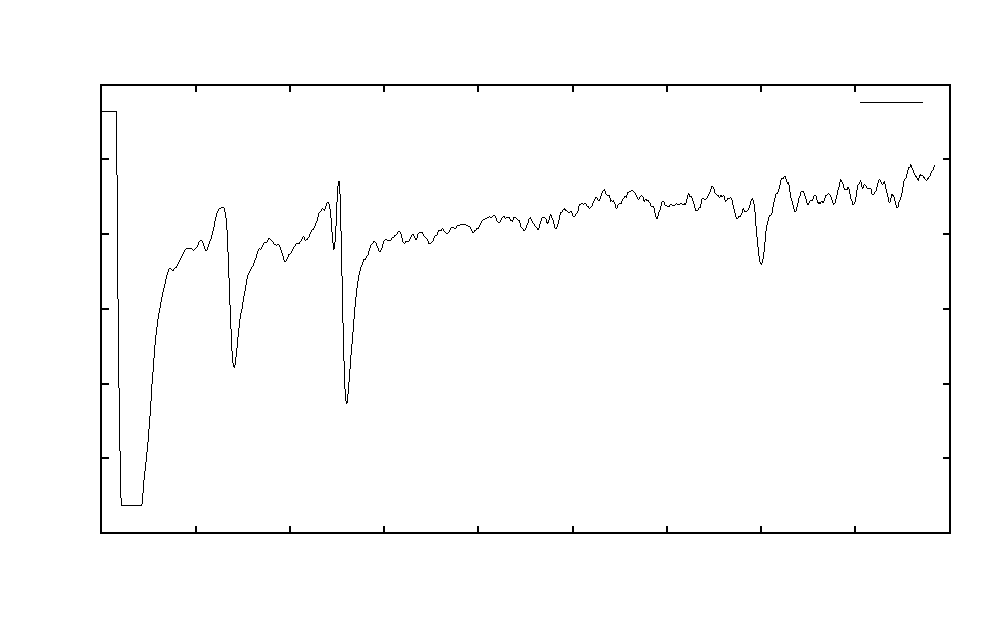
\includegraphics{ph2}}%
    \gplfronttext
  \end{picture}%
\endgroup

			\caption{\centering Parameter: Modulationsspannung 10V, AQ 6min, Empfindlichkeit 0.1mV, Zeitkonstante 3s, Phase 12^\circ}
		\end{figure}

		\begin{figure}[H]
			\center
			% GNUPLOT: LaTeX picture with Postscript
\begingroup
  \makeatletter
  \providecommand\color[2][]{%
    \GenericError{(gnuplot) \space\space\space\@spaces}{%
      Package color not loaded in conjunction with
      terminal option `colourtext'%
    }{See the gnuplot documentation for explanation.%
    }{Either use 'blacktext' in gnuplot or load the package
      color.sty in LaTeX.}%
    \renewcommand\color[2][]{}%
  }%
  \providecommand\includegraphics[2][]{%
    \GenericError{(gnuplot) \space\space\space\@spaces}{%
      Package graphicx or graphics not loaded%
    }{See the gnuplot documentation for explanation.%
    }{The gnuplot epslatex terminal needs graphicx.sty or graphics.sty.}%
    \renewcommand\includegraphics[2][]{}%
  }%
  \providecommand\rotatebox[2]{#2}%
  \@ifundefined{ifGPcolor}{%
    \newif\ifGPcolor
    \GPcolorfalse
  }{}%
  \@ifundefined{ifGPblacktext}{%
    \newif\ifGPblacktext
    \GPblacktexttrue
  }{}%
  % define a \g@addto@macro without @ in the name:
  \let\gplgaddtomacro\g@addto@macro
  % define empty templates for all commands taking text:
  \gdef\gplbacktext{}%
  \gdef\gplfronttext{}%
  \makeatother
  \ifGPblacktext
    % no textcolor at all
    \def\colorrgb#1{}%
    \def\colorgray#1{}%
  \else
    % gray or color?
    \ifGPcolor
      \def\colorrgb#1{\color[rgb]{#1}}%
      \def\colorgray#1{\color[gray]{#1}}%
      \expandafter\def\csname LTw\endcsname{\color{white}}%
      \expandafter\def\csname LTb\endcsname{\color{black}}%
      \expandafter\def\csname LTa\endcsname{\color{black}}%
      \expandafter\def\csname LT0\endcsname{\color[rgb]{1,0,0}}%
      \expandafter\def\csname LT1\endcsname{\color[rgb]{0,1,0}}%
      \expandafter\def\csname LT2\endcsname{\color[rgb]{0,0,1}}%
      \expandafter\def\csname LT3\endcsname{\color[rgb]{1,0,1}}%
      \expandafter\def\csname LT4\endcsname{\color[rgb]{0,1,1}}%
      \expandafter\def\csname LT5\endcsname{\color[rgb]{1,1,0}}%
      \expandafter\def\csname LT6\endcsname{\color[rgb]{0,0,0}}%
      \expandafter\def\csname LT7\endcsname{\color[rgb]{1,0.3,0}}%
      \expandafter\def\csname LT8\endcsname{\color[rgb]{0.5,0.5,0.5}}%
    \else
      % gray
      \def\colorrgb#1{\color{black}}%
      \def\colorgray#1{\color[gray]{#1}}%
      \expandafter\def\csname LTw\endcsname{\color{white}}%
      \expandafter\def\csname LTb\endcsname{\color{black}}%
      \expandafter\def\csname LTa\endcsname{\color{black}}%
      \expandafter\def\csname LT0\endcsname{\color{black}}%
      \expandafter\def\csname LT1\endcsname{\color{black}}%
      \expandafter\def\csname LT2\endcsname{\color{black}}%
      \expandafter\def\csname LT3\endcsname{\color{black}}%
      \expandafter\def\csname LT4\endcsname{\color{black}}%
      \expandafter\def\csname LT5\endcsname{\color{black}}%
      \expandafter\def\csname LT6\endcsname{\color{black}}%
      \expandafter\def\csname LT7\endcsname{\color{black}}%
      \expandafter\def\csname LT8\endcsname{\color{black}}%
    \fi
  \fi
  \setlength{\unitlength}{0.0500bp}%
  \begin{picture}(9354.00,5102.00)%
    \gplgaddtomacro\gplbacktext{%
      \csname LTb\endcsname%
      \put(682,704){\makebox(0,0)[r]{\strut{}-6}}%
      \put(682,1171){\makebox(0,0)[r]{\strut{}-5}}%
      \put(682,1638){\makebox(0,0)[r]{\strut{}-4}}%
      \put(682,2105){\makebox(0,0)[r]{\strut{}-3}}%
      \put(682,2573){\makebox(0,0)[r]{\strut{}-2}}%
      \put(682,3040){\makebox(0,0)[r]{\strut{}-1}}%
      \put(682,3507){\makebox(0,0)[r]{\strut{} 0}}%
      \put(682,3974){\makebox(0,0)[r]{\strut{} 1}}%
      \put(682,4441){\makebox(0,0)[r]{\strut{} 2}}%
      \put(814,484){\makebox(0,0){\strut{} 0}}%
      \put(1900,484){\makebox(0,0){\strut{} 20}}%
      \put(2985,484){\makebox(0,0){\strut{} 40}}%
      \put(4071,484){\makebox(0,0){\strut{} 60}}%
      \put(5157,484){\makebox(0,0){\strut{} 80}}%
      \put(6243,484){\makebox(0,0){\strut{} 100}}%
      \put(7328,484){\makebox(0,0){\strut{} 120}}%
      \put(8414,484){\makebox(0,0){\strut{} 140}}%
      \put(176,2572){\rotatebox{-270}{\makebox(0,0){\strut{}$dN/dE \ [1]$}}}%
      \put(4885,154){\makebox(0,0){\strut{}$E \ [eV]$}}%
      \put(4885,4771){\makebox(0,0){\strut{}Probenhalter-Spektrum an Position (2)}}%
      \put(4505,1078){\makebox(0,0)[l]{\strut{}68}}%
    }%
    \gplgaddtomacro\gplfronttext{%
      \csname LTb\endcsname%
      \put(7970,4268){\makebox(0,0)[r]{\strut{}Messwerte}}%
    }%
    \gplbacktext
    \put(0,0){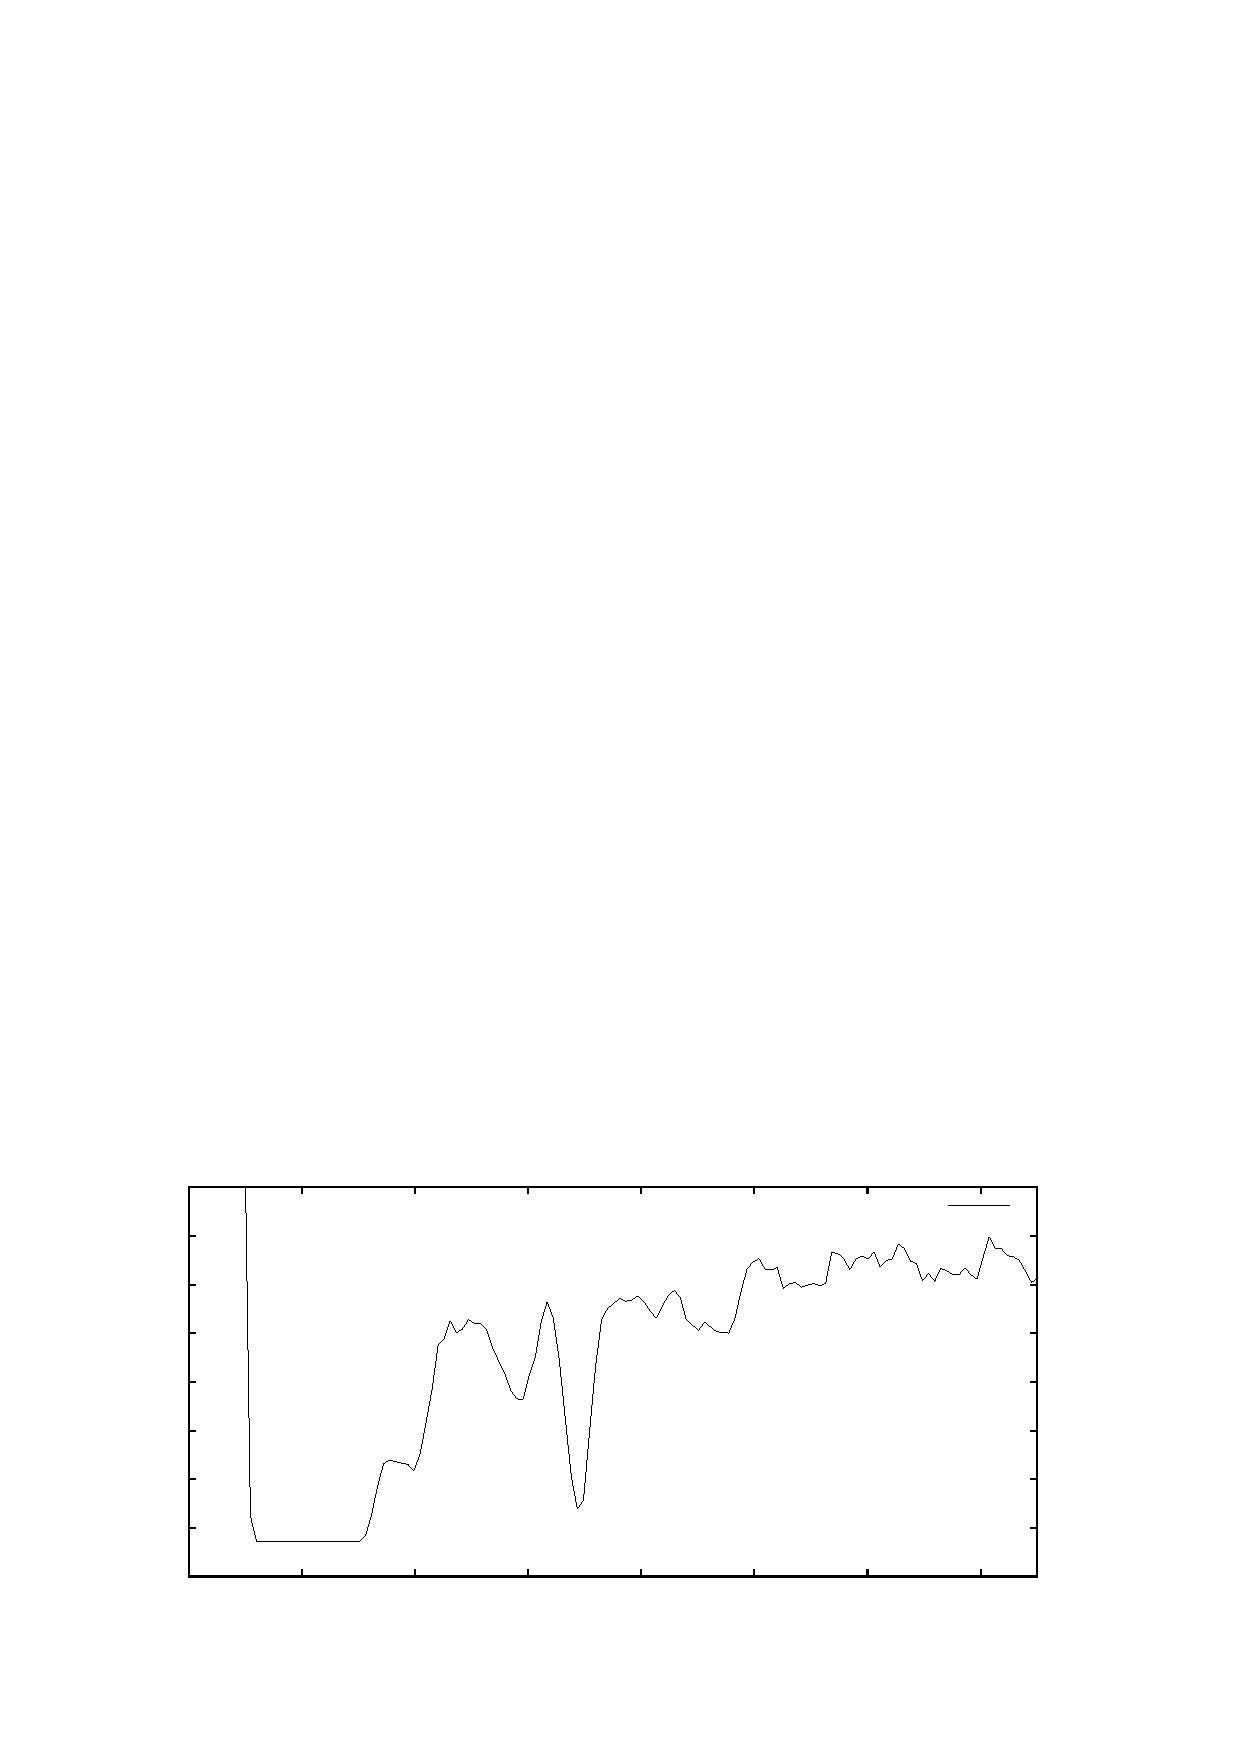
\includegraphics{ph4}}%
    \gplfronttext
  \end{picture}%
\endgroup

			\caption{\centering Parameter: Modulationsspannung 5V, AQ 60s, Empfindlichkeit 0.3mV, Zeitkonstante 300ms, Phase 12^\circ}
		\end{figure}

		Das erste Spektrum des Probenhalters zeigt drei ausgeprägte Minima.
		Diese wurden durch ein selbstgeschriebenes Programm ermittelt, wobei die jeweiligen Ergebnisse unterhalb der jeweiligen Peaks im Spektrum eingetragen wurden.
		Um auch den übersteuerten niederenergetischen Bereich zu vermessen wurde ein weiteres Spektrum mit geringerer Empfindlichkeit gemessen.

		Auch hier wurde der markanteste Peak markiert.
		Durch Vergleiche mit bereits vorhandenen Spektren aus \cite{handbook} (siehe Anhang), konnten folgende Elemente mit den jeweiligen Peak-Peak-Intensitäten nachgewiesen werden:

		\begin{description}
			\item[Kohlenstoff (C):] $4.29$ bei $282$eV (chemische Verschiebung des Energieniveaus)
			\item[Sauerstoff (O):] $5.97$ bei $520$eV (chemische Verschiebung des Energieniveaus)
			\item[Aluminium (Al):] $1.76$ bei $1399$eV
			\item[Aluminium (Al):] $4.32$ bei $68$eV (nicht mit den anderen Werten vergleichbar)
		\end{description}

		Berechnung der relativen Konzentrationen am Beispiel von Kohlenstoff (relative Empfindlichkeitsfaktoren aus \cite{article} entnommen):

		\begin{eqnarray*}
			c(C) &=& \dfrac{I(C)/S(C)}{I(C)/S(C) + I(O)/S(O) + I(Al)/S(Al)} \\
				&& \\
				&=& \dfrac{4.29/0.14}{4.29/0.14 + 5.97/0.40 + 4.32/0.19} \\
				&& \\
				&=& 0.55
		\end{eqnarray*}

		Analog folgt für alle gefundenen Elemente:
		\begin{itemize}
			\item 
				$c(C) = 0.55$
			\item
				$c(O) = 0.27$
			\item
				$c(Al) = 0.17$
		\end{itemize}

		Das Verhältnis von Aluminium zu Sauerstoff beträgt in etwa 2:3.
		Daraus lässt sich schließen, dass Aluminium und Sauerstoff in der Verbindung $Al_2O_3$ (Aluminiumoxid) an der Oberfläche vorkommen.
		Dies bestätigt, dass es sich bei dem Probenhalter um einen Großteil Aluminium handelt, da dieses an der Oberfläche immer eine Oxidschicht ausbildet.
		Aufgrund der chemischen Verschiebung des Kohlenstoff-Peaks ist zu erwarten, dass auch Kohlenstoff an der Oberfläche nur in gebundener Form vorliegt.
		Das hohe Vorkommen von Kohlenstoff deutet hier auf diverse Verunreinigungen des Probenhalters hin.

	% subsubsection probenhalter (end)

	\subsubsection{Probe 3} % (fold)
	\label{ssub:probe_3}
	
		\begin{figure}[H]
			\center
			% GNUPLOT: LaTeX picture with Postscript
\begingroup
  \makeatletter
  \providecommand\color[2][]{%
    \GenericError{(gnuplot) \space\space\space\@spaces}{%
      Package color not loaded in conjunction with
      terminal option `colourtext'%
    }{See the gnuplot documentation for explanation.%
    }{Either use 'blacktext' in gnuplot or load the package
      color.sty in LaTeX.}%
    \renewcommand\color[2][]{}%
  }%
  \providecommand\includegraphics[2][]{%
    \GenericError{(gnuplot) \space\space\space\@spaces}{%
      Package graphicx or graphics not loaded%
    }{See the gnuplot documentation for explanation.%
    }{The gnuplot epslatex terminal needs graphicx.sty or graphics.sty.}%
    \renewcommand\includegraphics[2][]{}%
  }%
  \providecommand\rotatebox[2]{#2}%
  \@ifundefined{ifGPcolor}{%
    \newif\ifGPcolor
    \GPcolorfalse
  }{}%
  \@ifundefined{ifGPblacktext}{%
    \newif\ifGPblacktext
    \GPblacktexttrue
  }{}%
  % define a \g@addto@macro without @ in the name:
  \let\gplgaddtomacro\g@addto@macro
  % define empty templates for all commands taking text:
  \gdef\gplbacktext{}%
  \gdef\gplfronttext{}%
  \makeatother
  \ifGPblacktext
    % no textcolor at all
    \def\colorrgb#1{}%
    \def\colorgray#1{}%
  \else
    % gray or color?
    \ifGPcolor
      \def\colorrgb#1{\color[rgb]{#1}}%
      \def\colorgray#1{\color[gray]{#1}}%
      \expandafter\def\csname LTw\endcsname{\color{white}}%
      \expandafter\def\csname LTb\endcsname{\color{black}}%
      \expandafter\def\csname LTa\endcsname{\color{black}}%
      \expandafter\def\csname LT0\endcsname{\color[rgb]{1,0,0}}%
      \expandafter\def\csname LT1\endcsname{\color[rgb]{0,1,0}}%
      \expandafter\def\csname LT2\endcsname{\color[rgb]{0,0,1}}%
      \expandafter\def\csname LT3\endcsname{\color[rgb]{1,0,1}}%
      \expandafter\def\csname LT4\endcsname{\color[rgb]{0,1,1}}%
      \expandafter\def\csname LT5\endcsname{\color[rgb]{1,1,0}}%
      \expandafter\def\csname LT6\endcsname{\color[rgb]{0,0,0}}%
      \expandafter\def\csname LT7\endcsname{\color[rgb]{1,0.3,0}}%
      \expandafter\def\csname LT8\endcsname{\color[rgb]{0.5,0.5,0.5}}%
    \else
      % gray
      \def\colorrgb#1{\color{black}}%
      \def\colorgray#1{\color[gray]{#1}}%
      \expandafter\def\csname LTw\endcsname{\color{white}}%
      \expandafter\def\csname LTb\endcsname{\color{black}}%
      \expandafter\def\csname LTa\endcsname{\color{black}}%
      \expandafter\def\csname LT0\endcsname{\color{black}}%
      \expandafter\def\csname LT1\endcsname{\color{black}}%
      \expandafter\def\csname LT2\endcsname{\color{black}}%
      \expandafter\def\csname LT3\endcsname{\color{black}}%
      \expandafter\def\csname LT4\endcsname{\color{black}}%
      \expandafter\def\csname LT5\endcsname{\color{black}}%
      \expandafter\def\csname LT6\endcsname{\color{black}}%
      \expandafter\def\csname LT7\endcsname{\color{black}}%
      \expandafter\def\csname LT8\endcsname{\color{black}}%
    \fi
  \fi
  \setlength{\unitlength}{0.0500bp}%
  \begin{picture}(9354.00,6802.00)%
    \gplgaddtomacro\gplbacktext{%
      \csname LTb\endcsname%
      \put(682,704){\makebox(0,0)[r]{\strut{}-4}}%
      \put(682,1248){\makebox(0,0)[r]{\strut{}-3}}%
      \put(682,1791){\makebox(0,0)[r]{\strut{}-2}}%
      \put(682,2335){\makebox(0,0)[r]{\strut{}-1}}%
      \put(682,2879){\makebox(0,0)[r]{\strut{} 0}}%
      \put(682,3423){\makebox(0,0)[r]{\strut{} 1}}%
      \put(682,3966){\makebox(0,0)[r]{\strut{} 2}}%
      \put(682,4510){\makebox(0,0)[r]{\strut{} 3}}%
      \put(682,5054){\makebox(0,0)[r]{\strut{} 4}}%
      \put(682,5597){\makebox(0,0)[r]{\strut{} 5}}%
      \put(682,6141){\makebox(0,0)[r]{\strut{} 6}}%
      \put(814,484){\makebox(0,0){\strut{} 0}}%
      \put(1719,484){\makebox(0,0){\strut{} 200}}%
      \put(2624,484){\makebox(0,0){\strut{} 400}}%
      \put(3528,484){\makebox(0,0){\strut{} 600}}%
      \put(4433,484){\makebox(0,0){\strut{} 800}}%
      \put(5338,484){\makebox(0,0){\strut{} 1000}}%
      \put(6243,484){\makebox(0,0){\strut{} 1200}}%
      \put(7147,484){\makebox(0,0){\strut{} 1400}}%
      \put(8052,484){\makebox(0,0){\strut{} 1600}}%
      \put(8957,484){\makebox(0,0){\strut{} 1800}}%
      \put(176,3422){\rotatebox{-270}{\makebox(0,0){\strut{}$dN/dE \ [1]$}}}%
      \put(4885,154){\makebox(0,0){\strut{}$E \ [eV]$}}%
      \put(4885,6471){\makebox(0,0){\strut{}Proben-Spektrum an Position (3)}}%
      \put(2081,2444){\makebox(0,0)[l]{\strut{}280}}%
      \put(1312,976){\makebox(0,0)[l]{\strut{}86}}%
      \put(3302,976){\makebox(0,0)[l]{\strut{}518}}%
      \put(8097,2988){\makebox(0,0)[l]{\strut{}1621}}%
    }%
    \gplgaddtomacro\gplfronttext{%
      \csname LTb\endcsname%
      \put(7970,5968){\makebox(0,0)[r]{\strut{}Messwerte}}%
    }%
    \gplbacktext
    \put(0,0){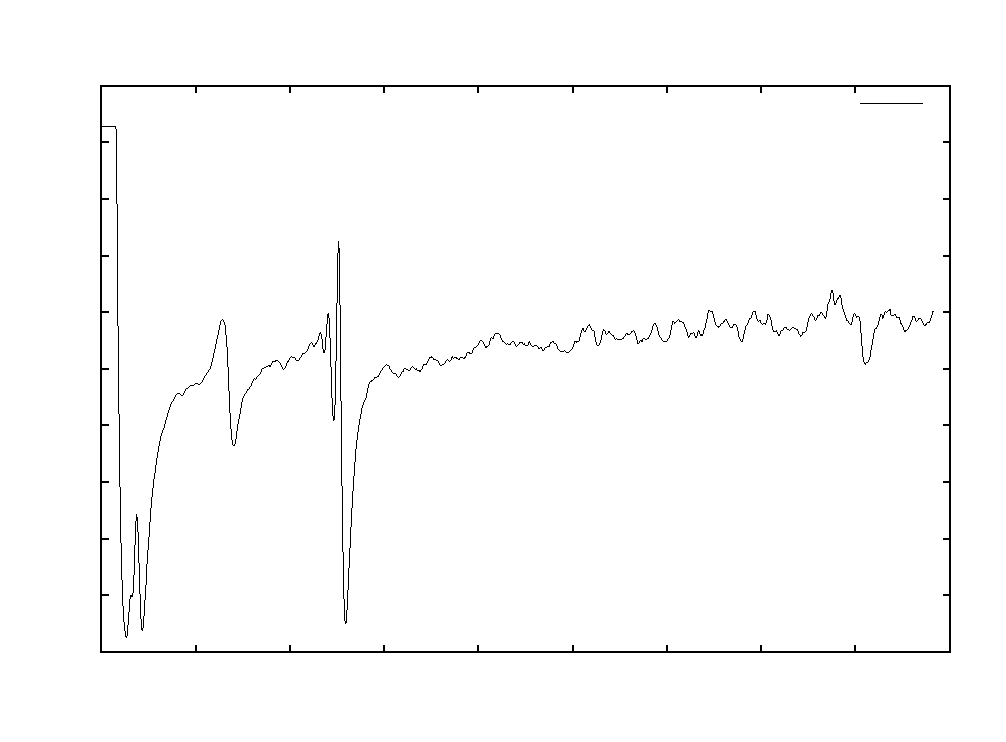
\includegraphics{ma05-03}}%
    \gplfronttext
  \end{picture}%
\endgroup

			\caption{\centering Parameter: Modulationsspannung 5V, AQ 6min, Empfindlichkeit 0.3mV, Zeitkonstante 3s, Phase 12^\circ}
		\end{figure}

		\begin{description}
			\item[Kohlenstoff (C):] $2.23$ bei $280$eV (chemische Verschiebung des Energieniveaus)
			\item[Sauerstoff (O):] $6.76$ bei $518$eV (chemische Verschiebung des Energieniveaus)
			\item[Silizium (Si):] $0.90$ bei $1621$eV
			\item[Silizium (Si):] $2.06$ bei $86$eV
		\end{description}

		Es folgt:

		\begin{itemize}
			\item 
				$c(C) = 0.44$
			\item
				$c(O) = 0.47$
			\item
				$c(Si) = 0.09$
		\end{itemize}

		Der Glanz der Probe auf dem fotografierten Bild und das Auftreten von Silizium und Sauerstoff könnten eine Zusammensetzung ähnlich von Glas ($SiO_2$) vermuten lassen.
		Jedoch zeigen die relativen Konzentrationen damit keine Übereinstimmung.
		Grundsätzlich kann die Probe durch Sauer- und Kohlenstoff auch stark verunreinigt sein. 
		Des Weiteren gibt es die Möglichkeit, das im nicht-aufgenommenen Bereich andere Peaks liegen, welche zusätzliche Aussagen über die Stoffzusammensetzung geben würden (maximaler Span: 2000V).
		Es ist uns nicht möglich anhand des gegebenen Spektrums weitere Aussagen über die Oberfläche der Probe zu treffen.

	% subsubsection probe_3 (end)

% subsection qualitative_analyse_der_proben (end)

\subsection{Einfluss des Elektronenstrahls auf die Probe} % (fold)
\label{sub:einfluss_des_elektronenstrahls_auf_die_probe}

	Folgendes Probenstrombild wurde vor der Messung eines Auger-Spektrums über Probe 3 aufgenommen:

	\begin{figure}[H]
		\center
		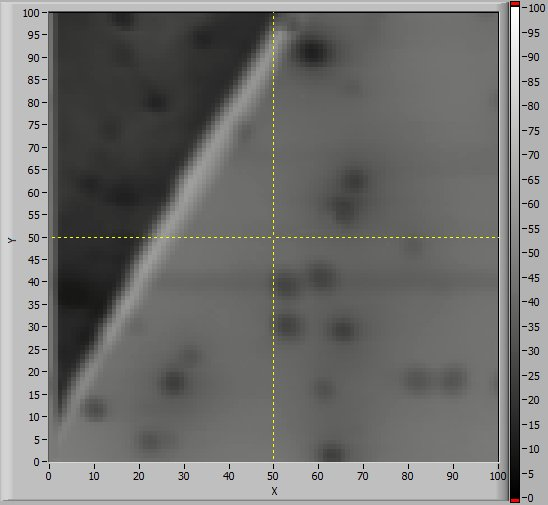
\includegraphics[scale=0.4]{voher.jpg}
		\caption{Probenstrombild der Probe 3 vor der Aufnahme eines Auger-Spektrums}
	\end{figure}

	Durch eine weitere Aufnahme eines Probenstrombilds nach der Messung war nun deutlich, dass der Elektronenstrahl die Oberfläche leicht verändert.

	\begin{figure}[H]
		\center
		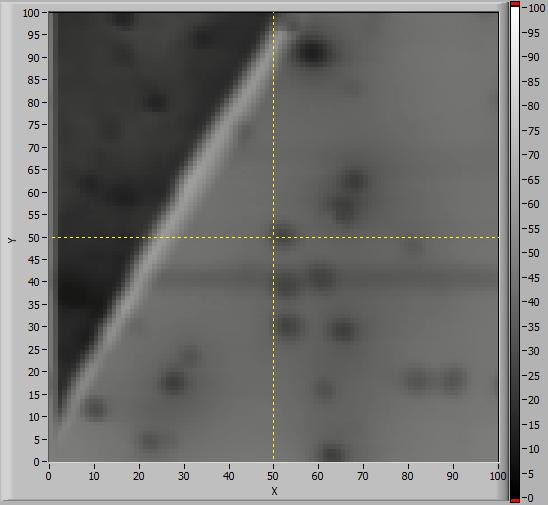
\includegraphics[scale=0.4]{nachher.jpg}
		\caption{Probenstrombild der Probe 3 nach der Aufnahme des Auger-Spektrums}
	\end{figure}

	Die dunkle Verfärbung bedeutet hierbei einen geringeren Probenstrom an der bestrahlten Stelle.
	Es fließen also nicht so viele Elektronen an dieser Stelle ab, wie vorher.
	Sie müssen aus diesem Grund stärker reflektiert werden.
	Dies deutet daraufhin, dass an der untersuchten Stelle das Material glatter geworden ist (bzw. von einer dünnen Verunreinigungsschicht befreit worden ist).

% subsection einfluss_des_elektronenstrahls_auf_die_probe (end)

\newpage

\subsection{Sputtering} % (fold)
\label{sub:sputtering}

	Zum Vergleich bereits oben gezeigtes Silber-Spektrum vor dem Ionenätzen:

	\begin{figure}[H]
		\center
		% GNUPLOT: LaTeX picture with Postscript
\begingroup
  \makeatletter
  \providecommand\color[2][]{%
    \GenericError{(gnuplot) \space\space\space\@spaces}{%
      Package color not loaded in conjunction with
      terminal option `colourtext'%
    }{See the gnuplot documentation for explanation.%
    }{Either use 'blacktext' in gnuplot or load the package
      color.sty in LaTeX.}%
    \renewcommand\color[2][]{}%
  }%
  \providecommand\includegraphics[2][]{%
    \GenericError{(gnuplot) \space\space\space\@spaces}{%
      Package graphicx or graphics not loaded%
    }{See the gnuplot documentation for explanation.%
    }{The gnuplot epslatex terminal needs graphicx.sty or graphics.sty.}%
    \renewcommand\includegraphics[2][]{}%
  }%
  \providecommand\rotatebox[2]{#2}%
  \@ifundefined{ifGPcolor}{%
    \newif\ifGPcolor
    \GPcolorfalse
  }{}%
  \@ifundefined{ifGPblacktext}{%
    \newif\ifGPblacktext
    \GPblacktexttrue
  }{}%
  % define a \g@addto@macro without @ in the name:
  \let\gplgaddtomacro\g@addto@macro
  % define empty templates for all commands taking text:
  \gdef\gplbacktext{}%
  \gdef\gplfronttext{}%
  \makeatother
  \ifGPblacktext
    % no textcolor at all
    \def\colorrgb#1{}%
    \def\colorgray#1{}%
  \else
    % gray or color?
    \ifGPcolor
      \def\colorrgb#1{\color[rgb]{#1}}%
      \def\colorgray#1{\color[gray]{#1}}%
      \expandafter\def\csname LTw\endcsname{\color{white}}%
      \expandafter\def\csname LTb\endcsname{\color{black}}%
      \expandafter\def\csname LTa\endcsname{\color{black}}%
      \expandafter\def\csname LT0\endcsname{\color[rgb]{1,0,0}}%
      \expandafter\def\csname LT1\endcsname{\color[rgb]{0,1,0}}%
      \expandafter\def\csname LT2\endcsname{\color[rgb]{0,0,1}}%
      \expandafter\def\csname LT3\endcsname{\color[rgb]{1,0,1}}%
      \expandafter\def\csname LT4\endcsname{\color[rgb]{0,1,1}}%
      \expandafter\def\csname LT5\endcsname{\color[rgb]{1,1,0}}%
      \expandafter\def\csname LT6\endcsname{\color[rgb]{0,0,0}}%
      \expandafter\def\csname LT7\endcsname{\color[rgb]{1,0.3,0}}%
      \expandafter\def\csname LT8\endcsname{\color[rgb]{0.5,0.5,0.5}}%
    \else
      % gray
      \def\colorrgb#1{\color{black}}%
      \def\colorgray#1{\color[gray]{#1}}%
      \expandafter\def\csname LTw\endcsname{\color{white}}%
      \expandafter\def\csname LTb\endcsname{\color{black}}%
      \expandafter\def\csname LTa\endcsname{\color{black}}%
      \expandafter\def\csname LT0\endcsname{\color{black}}%
      \expandafter\def\csname LT1\endcsname{\color{black}}%
      \expandafter\def\csname LT2\endcsname{\color{black}}%
      \expandafter\def\csname LT3\endcsname{\color{black}}%
      \expandafter\def\csname LT4\endcsname{\color{black}}%
      \expandafter\def\csname LT5\endcsname{\color{black}}%
      \expandafter\def\csname LT6\endcsname{\color{black}}%
      \expandafter\def\csname LT7\endcsname{\color{black}}%
      \expandafter\def\csname LT8\endcsname{\color{black}}%
    \fi
  \fi
  \setlength{\unitlength}{0.0500bp}%
  \begin{picture}(9354.00,5102.00)%
    \gplgaddtomacro\gplbacktext{%
      \csname LTb\endcsname%
      \put(946,704){\makebox(0,0)[r]{\strut{}-2}}%
      \put(946,1171){\makebox(0,0)[r]{\strut{}-1.5}}%
      \put(946,1638){\makebox(0,0)[r]{\strut{}-1}}%
      \put(946,2105){\makebox(0,0)[r]{\strut{}-0.5}}%
      \put(946,2573){\makebox(0,0)[r]{\strut{} 0}}%
      \put(946,3040){\makebox(0,0)[r]{\strut{} 0.5}}%
      \put(946,3507){\makebox(0,0)[r]{\strut{} 1}}%
      \put(946,3974){\makebox(0,0)[r]{\strut{} 1.5}}%
      \put(946,4441){\makebox(0,0)[r]{\strut{} 2}}%
      \put(1078,484){\makebox(0,0){\strut{} 0}}%
      \put(2391,484){\makebox(0,0){\strut{} 100}}%
      \put(3704,484){\makebox(0,0){\strut{} 200}}%
      \put(5018,484){\makebox(0,0){\strut{} 300}}%
      \put(6331,484){\makebox(0,0){\strut{} 400}}%
      \put(7644,484){\makebox(0,0){\strut{} 500}}%
      \put(8957,484){\makebox(0,0){\strut{} 600}}%
      \put(176,2572){\rotatebox{-270}{\makebox(0,0){\strut{}$dN/dE \ [1]$}}}%
      \put(5017,154){\makebox(0,0){\strut{}$E \ [eV]$}}%
      \put(5017,4771){\makebox(0,0){\strut{}Ag-Spektrum}}%
    }%
    \gplgaddtomacro\gplfronttext{%
      \csname LTb\endcsname%
      \put(7970,4268){\makebox(0,0)[r]{\strut{}Messwerte}}%
    }%
    \gplbacktext
    \put(0,0){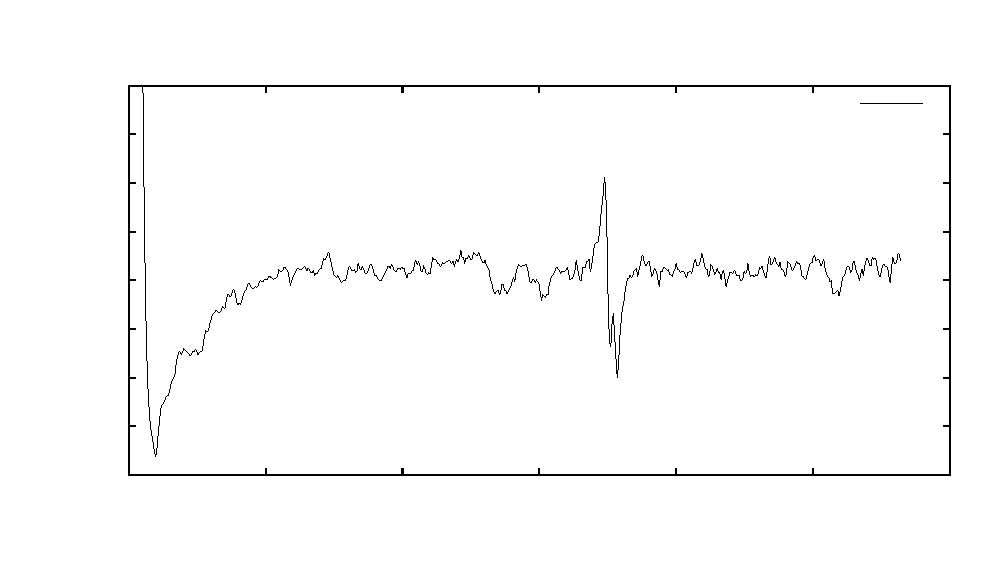
\includegraphics{ma03-16}}%
    \gplfronttext
  \end{picture}%
\endgroup

	\end{figure}

	Nach dem Sputtering:

	\begin{figure}[H]
		\center
		% GNUPLOT: LaTeX picture with Postscript
\begingroup
  \makeatletter
  \providecommand\color[2][]{%
    \GenericError{(gnuplot) \space\space\space\@spaces}{%
      Package color not loaded in conjunction with
      terminal option `colourtext'%
    }{See the gnuplot documentation for explanation.%
    }{Either use 'blacktext' in gnuplot or load the package
      color.sty in LaTeX.}%
    \renewcommand\color[2][]{}%
  }%
  \providecommand\includegraphics[2][]{%
    \GenericError{(gnuplot) \space\space\space\@spaces}{%
      Package graphicx or graphics not loaded%
    }{See the gnuplot documentation for explanation.%
    }{The gnuplot epslatex terminal needs graphicx.sty or graphics.sty.}%
    \renewcommand\includegraphics[2][]{}%
  }%
  \providecommand\rotatebox[2]{#2}%
  \@ifundefined{ifGPcolor}{%
    \newif\ifGPcolor
    \GPcolorfalse
  }{}%
  \@ifundefined{ifGPblacktext}{%
    \newif\ifGPblacktext
    \GPblacktexttrue
  }{}%
  % define a \g@addto@macro without @ in the name:
  \let\gplgaddtomacro\g@addto@macro
  % define empty templates for all commands taking text:
  \gdef\gplbacktext{}%
  \gdef\gplfronttext{}%
  \makeatother
  \ifGPblacktext
    % no textcolor at all
    \def\colorrgb#1{}%
    \def\colorgray#1{}%
  \else
    % gray or color?
    \ifGPcolor
      \def\colorrgb#1{\color[rgb]{#1}}%
      \def\colorgray#1{\color[gray]{#1}}%
      \expandafter\def\csname LTw\endcsname{\color{white}}%
      \expandafter\def\csname LTb\endcsname{\color{black}}%
      \expandafter\def\csname LTa\endcsname{\color{black}}%
      \expandafter\def\csname LT0\endcsname{\color[rgb]{1,0,0}}%
      \expandafter\def\csname LT1\endcsname{\color[rgb]{0,1,0}}%
      \expandafter\def\csname LT2\endcsname{\color[rgb]{0,0,1}}%
      \expandafter\def\csname LT3\endcsname{\color[rgb]{1,0,1}}%
      \expandafter\def\csname LT4\endcsname{\color[rgb]{0,1,1}}%
      \expandafter\def\csname LT5\endcsname{\color[rgb]{1,1,0}}%
      \expandafter\def\csname LT6\endcsname{\color[rgb]{0,0,0}}%
      \expandafter\def\csname LT7\endcsname{\color[rgb]{1,0.3,0}}%
      \expandafter\def\csname LT8\endcsname{\color[rgb]{0.5,0.5,0.5}}%
    \else
      % gray
      \def\colorrgb#1{\color{black}}%
      \def\colorgray#1{\color[gray]{#1}}%
      \expandafter\def\csname LTw\endcsname{\color{white}}%
      \expandafter\def\csname LTb\endcsname{\color{black}}%
      \expandafter\def\csname LTa\endcsname{\color{black}}%
      \expandafter\def\csname LT0\endcsname{\color{black}}%
      \expandafter\def\csname LT1\endcsname{\color{black}}%
      \expandafter\def\csname LT2\endcsname{\color{black}}%
      \expandafter\def\csname LT3\endcsname{\color{black}}%
      \expandafter\def\csname LT4\endcsname{\color{black}}%
      \expandafter\def\csname LT5\endcsname{\color{black}}%
      \expandafter\def\csname LT6\endcsname{\color{black}}%
      \expandafter\def\csname LT7\endcsname{\color{black}}%
      \expandafter\def\csname LT8\endcsname{\color{black}}%
    \fi
  \fi
  \setlength{\unitlength}{0.0500bp}%
  \begin{picture}(9354.00,5102.00)%
    \gplgaddtomacro\gplbacktext{%
      \csname LTb\endcsname%
      \put(682,704){\makebox(0,0)[r]{\strut{}-4}}%
      \put(682,1078){\makebox(0,0)[r]{\strut{}-3}}%
      \put(682,1451){\makebox(0,0)[r]{\strut{}-2}}%
      \put(682,1825){\makebox(0,0)[r]{\strut{}-1}}%
      \put(682,2199){\makebox(0,0)[r]{\strut{} 0}}%
      \put(682,2573){\makebox(0,0)[r]{\strut{} 1}}%
      \put(682,2946){\makebox(0,0)[r]{\strut{} 2}}%
      \put(682,3320){\makebox(0,0)[r]{\strut{} 3}}%
      \put(682,3694){\makebox(0,0)[r]{\strut{} 4}}%
      \put(682,4067){\makebox(0,0)[r]{\strut{} 5}}%
      \put(682,4441){\makebox(0,0)[r]{\strut{} 6}}%
      \put(814,484){\makebox(0,0){\strut{} 0}}%
      \put(2171,484){\makebox(0,0){\strut{} 100}}%
      \put(3528,484){\makebox(0,0){\strut{} 200}}%
      \put(4886,484){\makebox(0,0){\strut{} 300}}%
      \put(6243,484){\makebox(0,0){\strut{} 400}}%
      \put(7600,484){\makebox(0,0){\strut{} 500}}%
      \put(8957,484){\makebox(0,0){\strut{} 600}}%
      \put(176,2572){\rotatebox{-270}{\makebox(0,0){\strut{}$dN/dE \ [1]$}}}%
      \put(4885,154){\makebox(0,0){\strut{}$E \ [eV]$}}%
      \put(4885,4771){\makebox(0,0){\strut{}Silber-Spektrum nach Sputtering}}%
    }%
    \gplgaddtomacro\gplfronttext{%
      \csname LTb\endcsname%
      \put(7970,4268){\makebox(0,0)[r]{\strut{}Messwerte}}%
    }%
    \gplbacktext
    \put(0,0){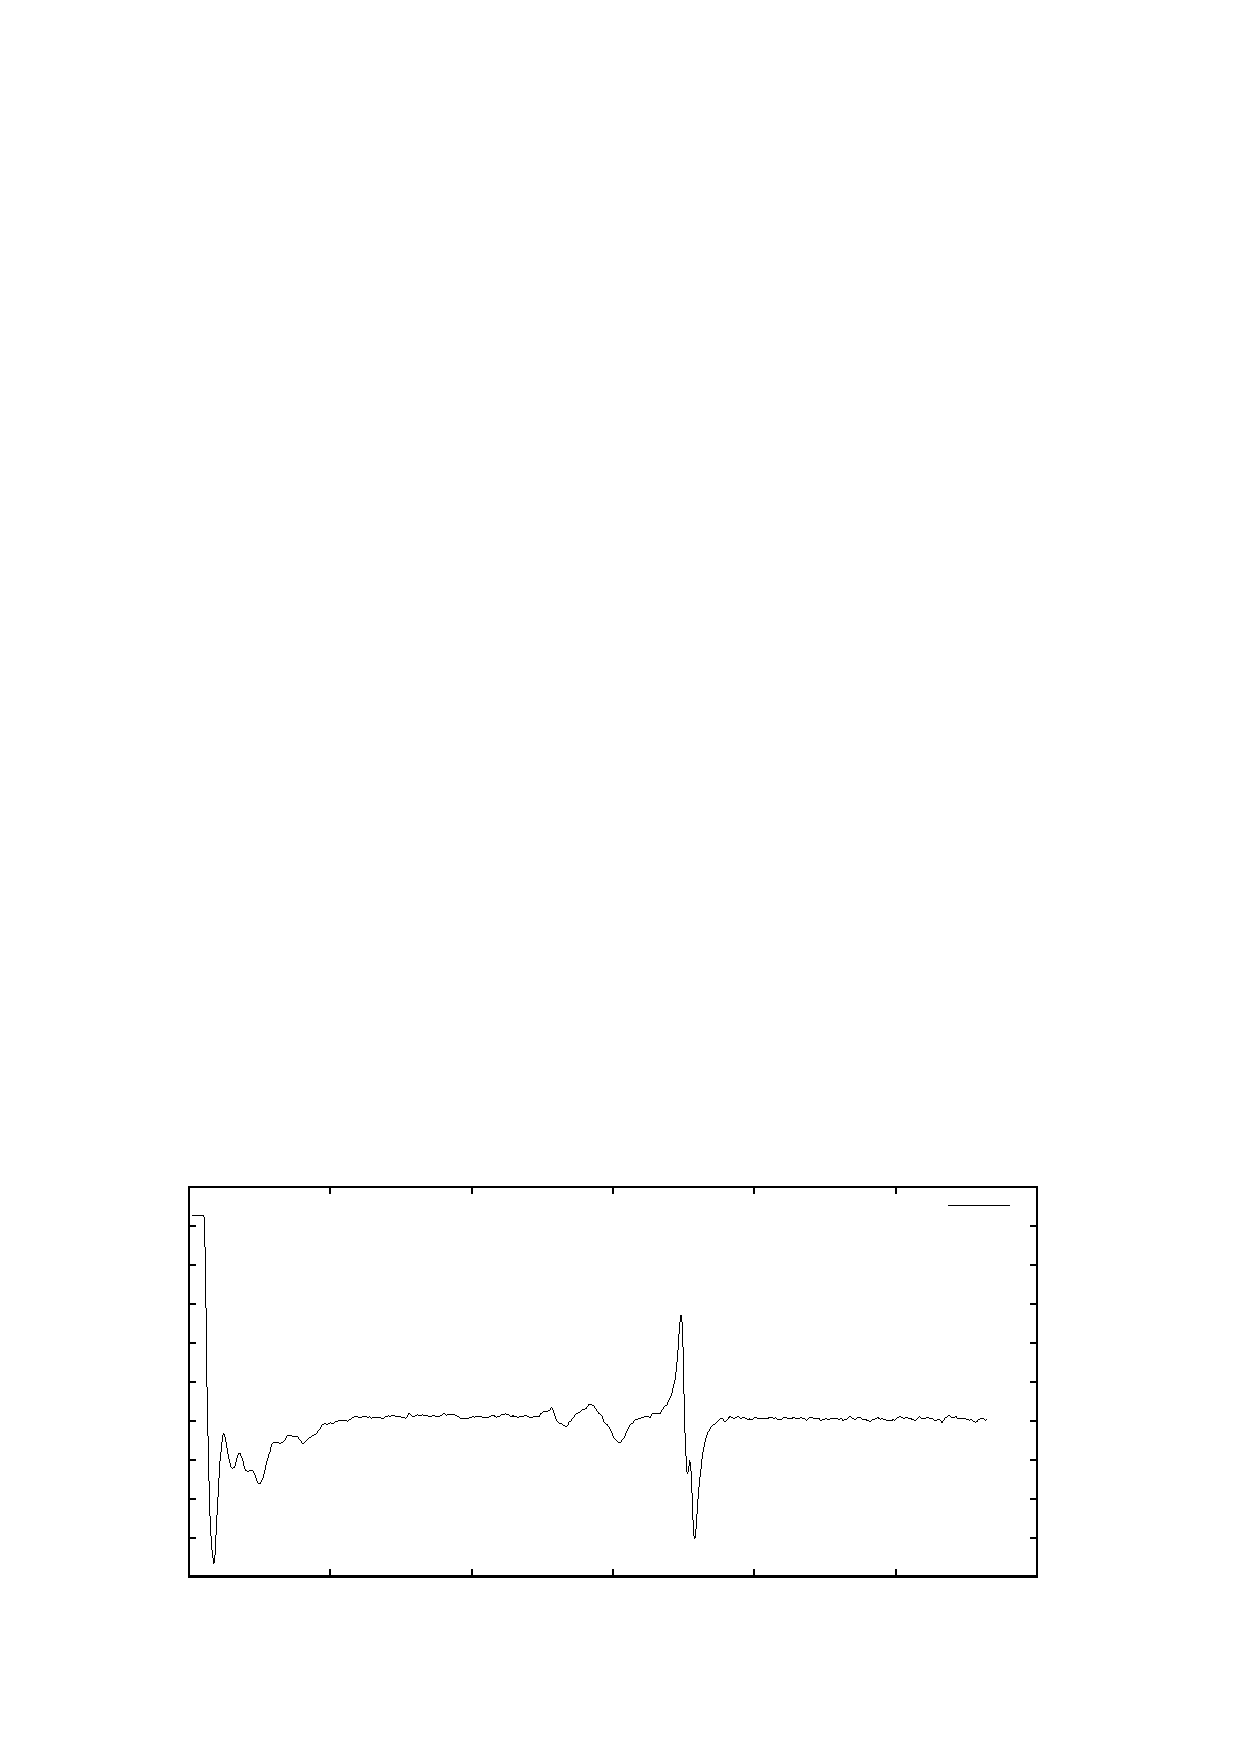
\includegraphics{agg}}%
    \gplfronttext
  \end{picture}%
\endgroup

		\caption{\centering Parameter: Modulationsspannung 2V, AQ 4min, Empfindlichkeit 1mV, Zeitkonstante 1s, Phase 12^\circ }
	\end{figure}

	Die stark geglättete Kurve zeigt, dass durch das Ionenätzen viele Verunreinigungen und Spurenelemente von der Oberfläche entfernt werden konnten, 
	sodass außer den charakteristischen Silberpeaks kaum noch andere Signale auftreten.


% subsection sputtering (end)
	\newpage
	Im Versuch sollten sich intensiv mit den Möglichkeiten und Anforderungen der Auger-Elektronen-Spektroskopie auseinandergesetzt werden.
Es zeigte sich, dass die AES ein sehr empfindliches und auch aufwendiges Verfahren zur Oberflächenanalyse darstellt, dass bei langer Messzeit, optimalen Parametern und hoher Sauberkeit der Probe auch sehr kleine Konzentrationen von Elementen auf der Oberfläche nachweisen kann. Die erwarteten Peaks von Silber, Sauerstoff, Kohlenstoff und Aluminium stimmten alle in geringen Toleranzbereichen mit den Tabellenwerten überein. 
Abweichungen ergaben sich vor allem in der Form und erwarteten Intensität der Peaks.
So zeigte Sauerstoff oft eine größere Asymmetrie auf, während sie bei Kohlenstoff fehlte. Auch der Doppelausschlag bei Silber zeigte in der Mitte nicht die erwartete Intensität. Dennoch muss man sagen, das im qualitativen Bereich gute Analysen der jeweiligen Proben vorgenommen werden konnten.
Die qualitative Analyse war aufgrund der oft von einer auf die nächste Messung wechselnden Intensitäten und unklaren Peak Abgrenzungen eher schwierig und uneindeutig. Hierfür sind längere Messungen und größere Probenströme notwendig.
Überraschend war das hohe Vorkommen von Kohlenstoff auf fast jeder Probe. Aus diesem Grund halten wir Sputtern vor jeder genaueren Spektroskopie für notwendig.
	\newpage
	\section{Verwendete Quellen} % (fold)
\label{sec:verwendete_quellen}

	\begin{itemize}
		\setlength\itemsep{1em}
		\item Gerthsen Physik 24.Auflage
		\item Hunklinger Festkörperphysik
		\item de.wikipedia.org/wiki/CCD-Sensor
		\item Versuchsunterlagen Spektroskopie der Sonne
	\end{itemize}

% section verwendete_quellen (end)
	\newpage

	\appendix

	\section{Vergleichsspektren} % (fold)
	\label{sec:vergleichsspektren}
	
		\begin{figure}[H]
			\center
			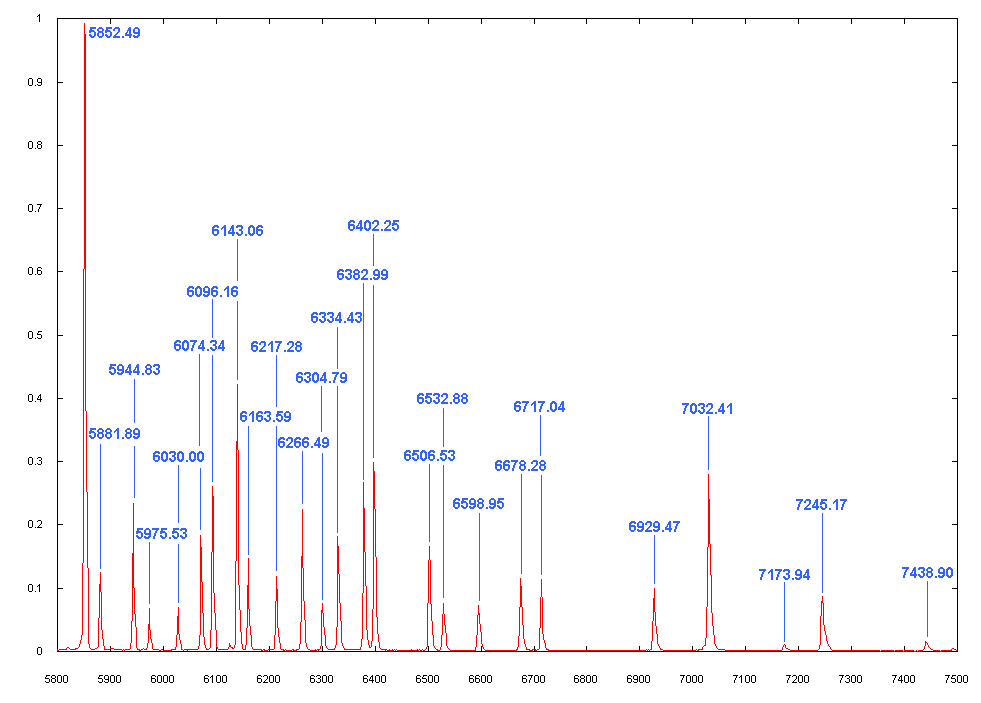
\includegraphics[scale=0.45, angle=-90]{referenzen/ne-light-spec.png}
			\caption{Spektrum einer Neon-Glimmlampe,  Quelle: Versuchsunterlagen}
			\label{fig:ne-light-spec}
		\end{figure}

		\begin{figure}[H]
			\center
			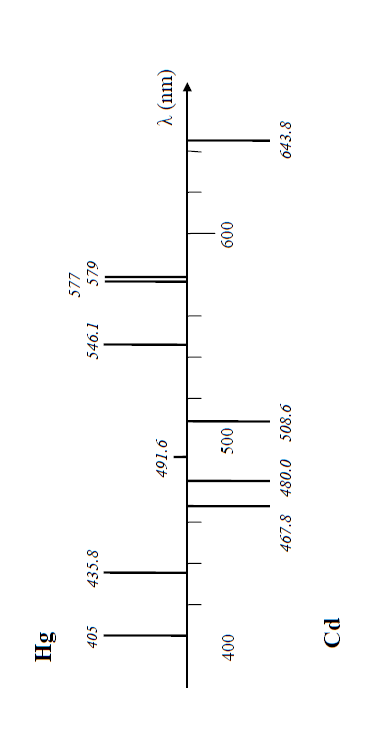
\includegraphics[scale=1, angle=-180]{referenzen/hg-cd-reference.PNG}
			\caption{Spektrum einer Quecksilber-Cadmium-Entladungslampe, Quelle: Versuchsunterlagen}
			\label{fig:hg-light-spec}
		\end{figure}

	% section vergleichsspektren (end)

	\section{Beispiele des Sonnenspektrums} % (fold)
	\label{sec:beispiele_des_sonnenspektrums}
	
		\begin{figure}[H]
			\center
			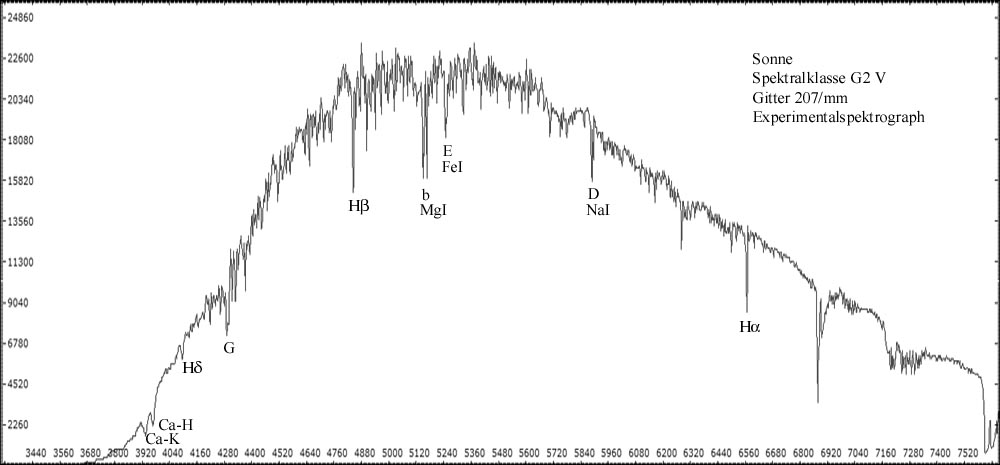
\includegraphics[scale=0.5, angle=-90]{referenzen/sonnenspektrum-1.jpg}
			\caption{Beispiel eines Sonnnenspektrums \\ Quelle: http://www.sternwarte-habichtswald.de/astromania/\ galerie/Spektren/Sonne-grafik.jpg}
			\label{fig:sonnenspektrum-1}
		\end{figure}

		\begin{figure}
			\center
			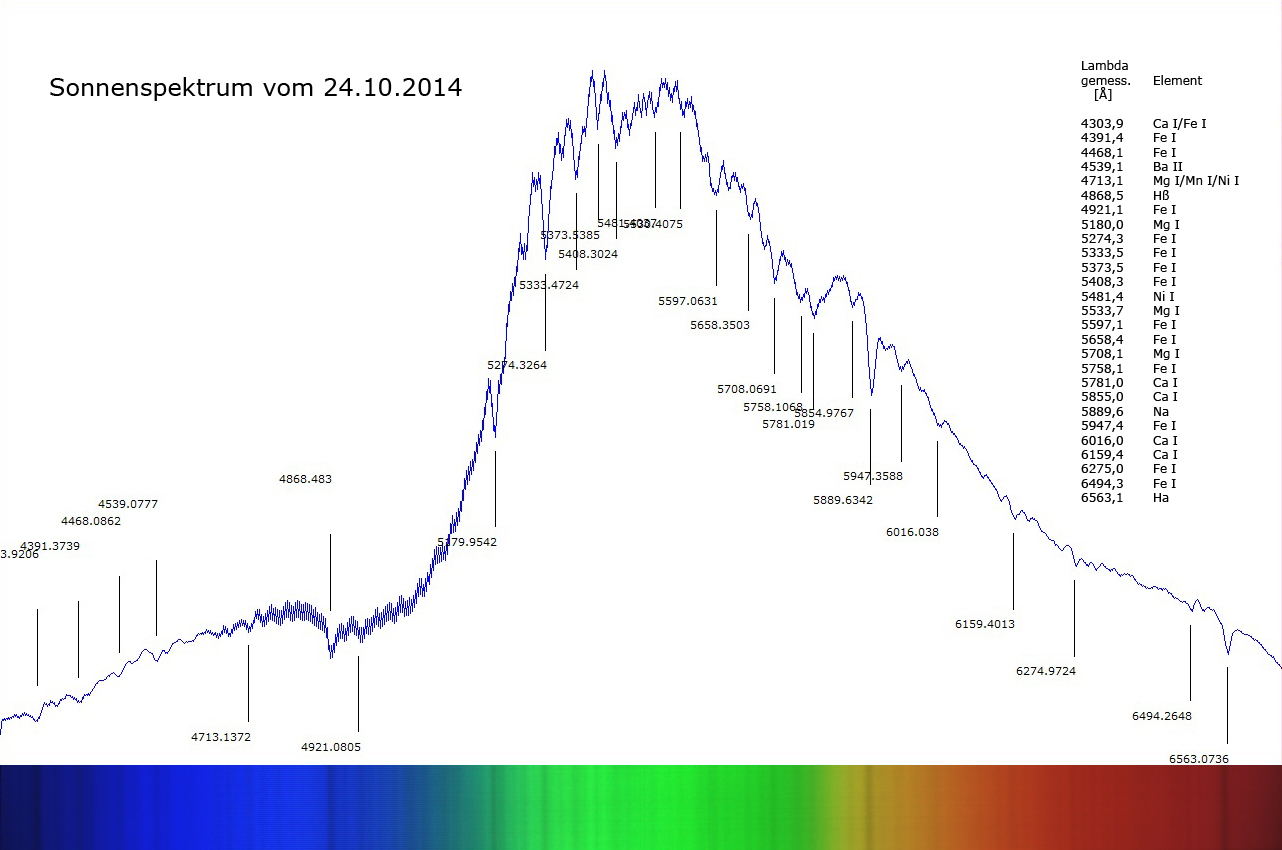
\includegraphics[scale=0.4, angle=-90]{referenzen/sonnenspektrum-2.jpg}
			\caption{Beispiel eines Sonnenspektrums \\ Quelle: http://www.deep-sky-images.de/albums/userpics/10002/\ Sonnenspektrum\_text.jpg}
			\label{fig:sonnenspektrum-2}
		\end{figure}

	% section beispiele_des_sonnenspektrums (end)

	\section{Kenngrößen des Gitterspektrographen} % (fold)
	\label{sec:kenngr_en_des_gitterspektrographen}
	
		\begin{figure}[H]
			\center
			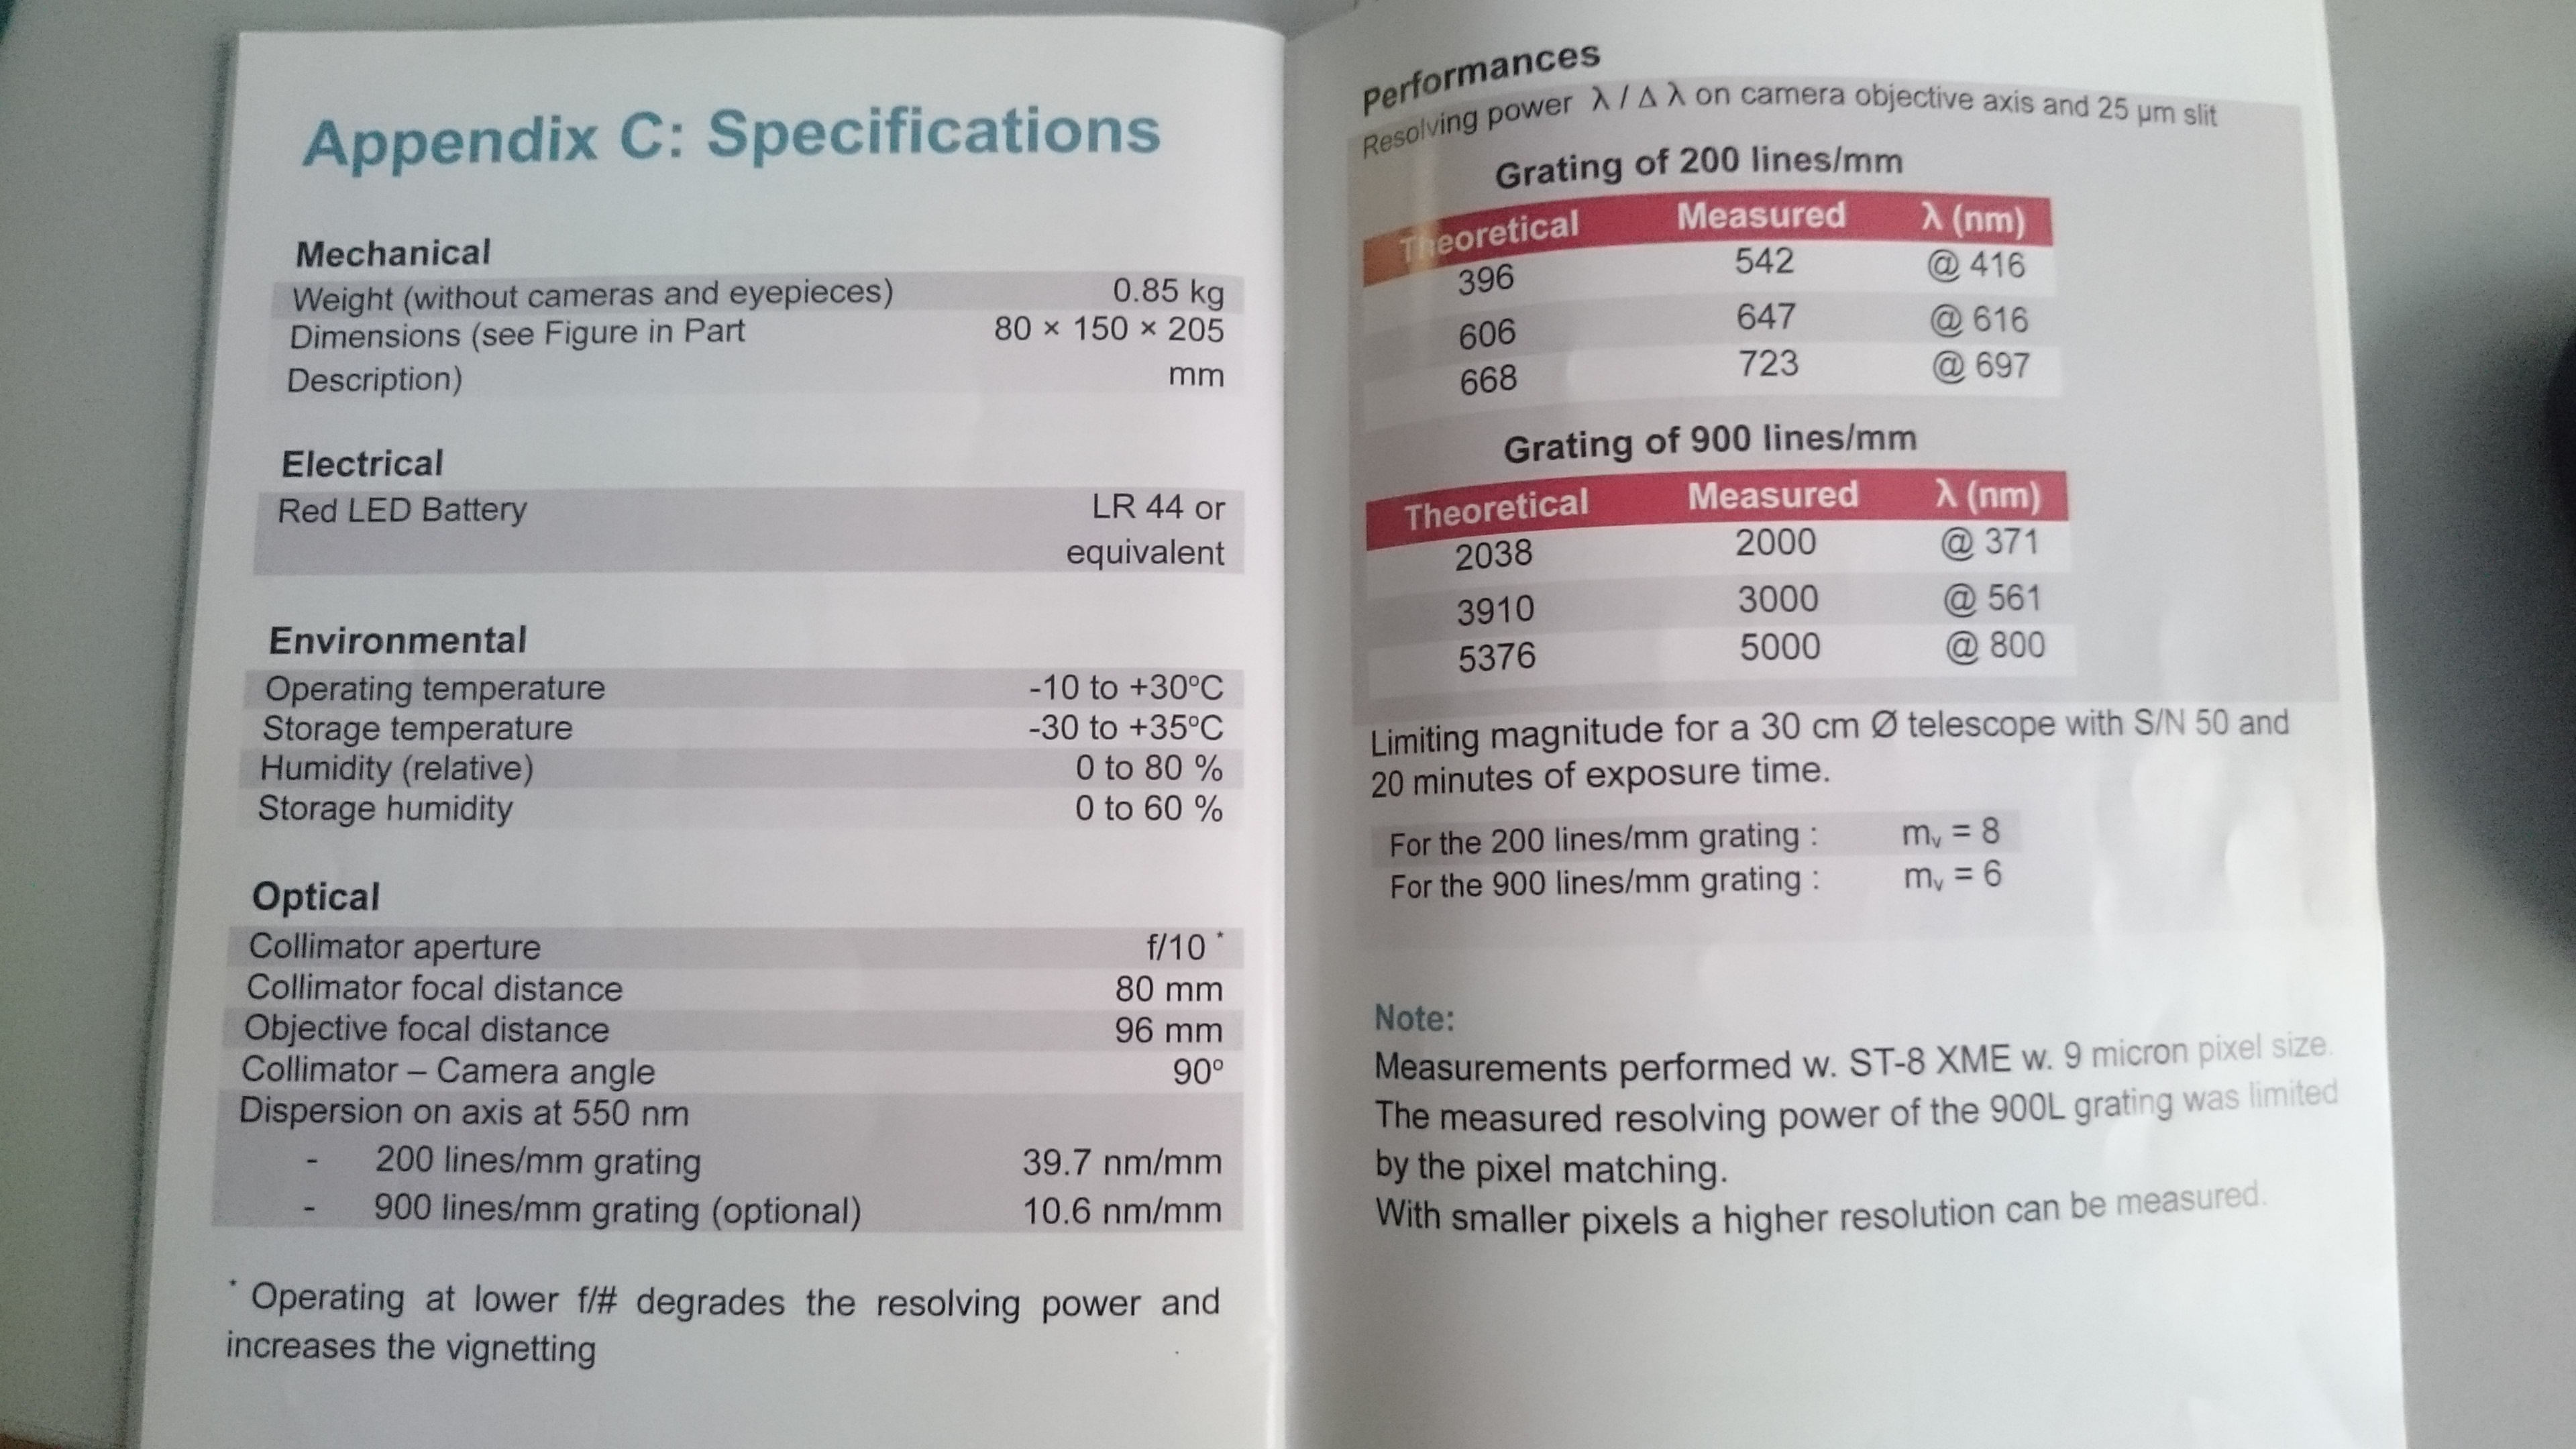
\includegraphics[scale=0.085, angle=0]{referenzen/DSC_0689.JPG}
			\caption{Herstellerangaben zum Gitterspektrometer \\ Quelle: Unterlagen am Versuchsplatz}
			\label{fig:sonnenspektrum-1}
		\end{figure}

		\begin{figure}[H]
			\center
			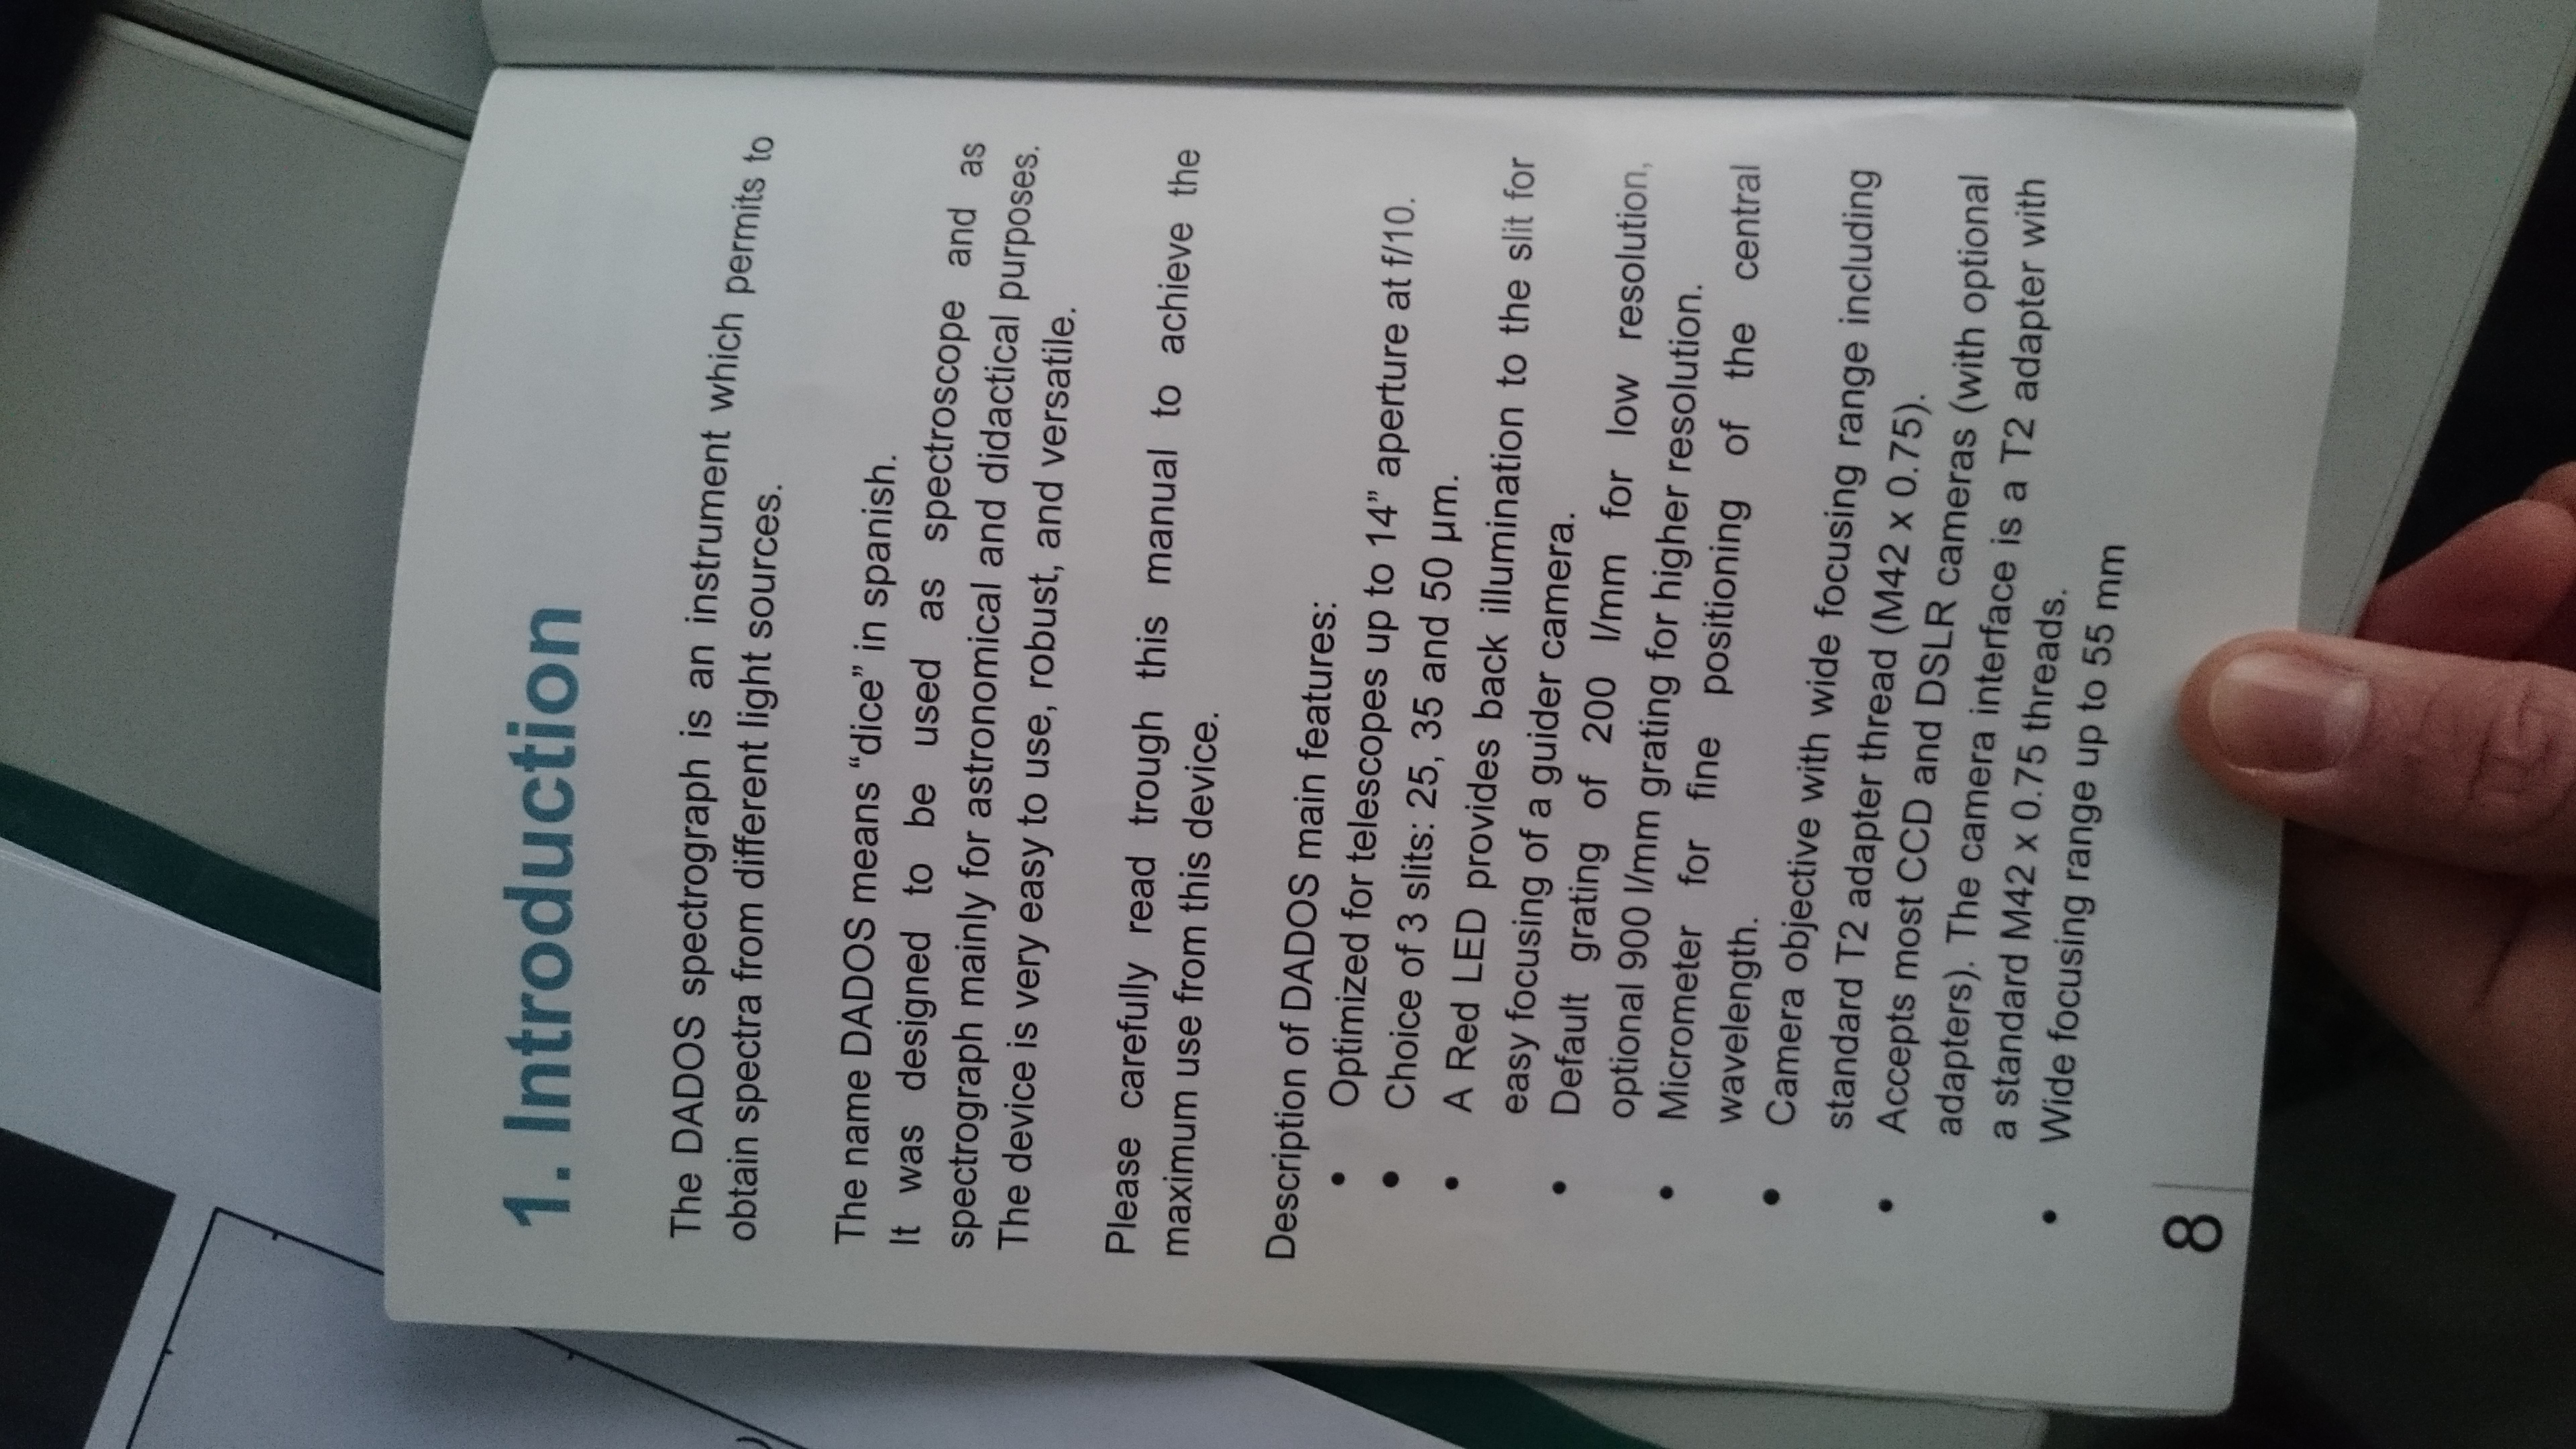
\includegraphics[scale=0.085, angle=0]{referenzen/DSC_0690.JPG}
			\caption{Herstellerangaben zum Gitterspektrometer \\ Quelle: Unterlagen am Versuchsplatz}
			\label{fig:sonnenspektrum-1}
		\end{figure}
	% section kenngr_en_des_gitterspektrographen (end)

\end{document}